\documentclass{tuna-report}
\usepackage{codespace}
\usepackage{caption}
\usepackage{subcaption}
\usepackage{wrapfig}
\usepackage{graphicx}
\usepackage{array}
\usepackage[super]{nth}
\usepackage{longtable}
\usepackage{listings} % For code snippets 
\usepackage{tikz}
\usetikzlibrary{calc}

\usepackage[inkscapearea=page]{svg}	% import svg images
\usepackage{makecell} % force line break in a cell of a table
\usepackage[raggedrightboxes]{ragged2e} % justify word behavior in a table cell

% \usepackage[colorlinks]{hyperref}
%\usepackage[printonlyused,withpage]{acronym} %abbreviations
\usepackage{acro}
% Sub-preambles
% https://github.com/MartinScharrer/standalone

% Encodings
\usepackage{gensymb,textcomp}

% Better tables
% Wide tables go to https://tex.stackexchange.com/q/332902
\usepackage{array,multicol,multirow,siunitx,tabularx}

% Better enum
\usepackage{enumitem}

% Graphics
\usepackage{caption,float}

% Allow setting >max< width of figure
% 'export' allows adjustbox keys in \includegraphics
% For demonstration purposes, remove in production
\usepackage[export]{adjustbox}

% For demonstration purposes, remove in production
\usepackage{mwe}


% Configurations
\newcounter{memberrowno}
\setcounter{memberrowno}{0}
\setcounter{tocdepth}{5}
\reportlayout%

% Override (some) default values
\ocoursename{Practical Training Report}
\title{Practical Training Report}
% \oadvisor{Prof. Christina Andersson, Prof. Dr. Tine Köhler, Prof. Dr. Sebhatleab Tewolde Kelat}

% ================== Custom commands
\newcommand*\mean[1]{\bar{#1}}

% Set up the command for a blank page
\usepackage{afterpage}

\newcommand\blankpage{%
    \null
    \
    \vfil
    \hfil (Intentionally left blank) \hfil
    \vfil
    \thispagestyle{empty}%
    % \addtocounter{page}{-1}%
    \newpage}
    
%   Make /bigcdot
\makeatletter
\newcommand*\bigcdot{\mathpalette\bigcdot@{.5}}
\newcommand*\bigcdot@[2]{\mathbin{\vcenter{\hbox{\scalebox{#2}{$\m@th#1\bullet$}}}}}
\makeatother
    
   
% ========================================

\graphicspath{ {graphics/} }

% Disable hypcap for specific captions
\captionsetup[figure]{hypcap=false}

% =================DECLARE ACRONYMS=======================

\DeclareAcronym{cse}{
	short=CSE,
	long=Computer Science and Engineering,
}

\DeclareAcronym{api}{
	short=API,
	long=Application Programming Interface,
}

\DeclareAcronym{vgu}{
	short=VGU,
	long=Vietnamese-German University,
}

\DeclareAcronym{jwt}{
	short=JWT,
	long=JSON Web Token,
}

\DeclareAcronym{ui}{
	short=UI,
	long=User Interface,
}


\DeclareAcronym{rest}{
	short=REST,
	long=Representational State Transfer,
}

\DeclareAcronym{ai}{
	short=AI,
	long=Artificial Intelligence,
}

\DeclareAcronym{sql}{
	short=SQL,
	long=Structured Query Language,
}

% ================ STYLE FOR JS PROGRAMMING LANGUAGE ===============
\usepackage{xcolor}

\definecolor{codegreen}{rgb}{0,0.6,0}
\definecolor{codegray}{rgb}{0.5,0.5,0.5}
\definecolor{codepurple}{rgb}{0.58,0,0.82}
\definecolor{backcolour}{rgb}{0.95,0.95,0.92}
\definecolor{magenta}{rgb}{1,0,1} % Magenta for JavaScript keywords


% Define JavaScript as a language in listings
\lstdefinelanguage{JavaScript}{
	keywords={break, case, catch, continue, debugger, default, delete, do, else, finally, for, function, if, in, instanceof, new, return, switch, this, throw, try, typeof, var, let, const, while, with, yield, async, await, of},
	keywordstyle=\color{magenta}\bfseries, % Magenta for keywords
	ndkeywords={class, export, boolean, throw, implements, import, this},
	ndkeywordstyle=\color{magenta}, % Magenta for additional keywords
	identifierstyle=\color{black},  % Default color for variables
	sensitive=true,                 % Case-sensitive
	comment=[l]{//},                % Single-line comments
	morecomment=[s]{/*}{*/},        % Multi-line comments
	commentstyle=\color{codegreen}\ttfamily, % Comments in green
	stringstyle=\color{codepurple},          % Strings in purple
	morestring=[b]',                % Single quotes for strings
	morestring=[b]"                 % Double quotes for strings
}


\lstset{
	language=JavaScript,               % Set JavaScript as the language
	backgroundcolor=\color{backcolour},   
	commentstyle=\color{codegreen},
	keywordstyle=\color{magenta},
	numberstyle=\tiny\color{codegray},
	stringstyle=\color{codepurple},
	basicstyle=\ttfamily\footnotesize,
	breakatwhitespace=false,         
	breaklines=true,                 
	captionpos=b,                    
	keepspaces=true,                 
	numbers=left,                    
	numbersep=5pt,                  
	showspaces=false,                
	showstringspaces=false,
	showtabs=false,                  
	tabsize=2,
	frame=single
}

\renewcommand{\lstlistingname}{Code snippet}	% For lisitngs caption name
\renewcommand{\lstlistlistingname}{List of Code Snippets}	% For codes listing table title

% ========================= BEGIN DOCUMENT =======================
\begin{document}
	
	
\begin{titlepage}
	\begin{tikzpicture}[remember picture,overlay,inner sep=0,outer sep=0]
		\draw[black!70!black,line width=4pt] ([xshift=-1.5cm,yshift=-2cm]current page.north east) coordinate (A)--([xshift=1.5cm,yshift=-2cm]current page.north west) coordinate(B)--([xshift=1.5cm,yshift=2cm]current page.south west) coordinate (C)--([xshift=-1.5cm,yshift=2cm]current page.south east) coordinate(D)--cycle;
		
		\draw ([yshift=0.5cm,xshift=-0.5cm]A)-- ([yshift=0.5cm,xshift=0.5cm]B)--
		([yshift=-0.5cm,xshift=0.5cm]B) --([yshift=-0.5cm,xshift=-0.5cm]B)--([yshift=0.5cm,xshift=-0.5cm]C)--([yshift=0.5cm,xshift=0.5cm]C)--([yshift=-0.5cm,xshift=0.5cm]C)-- ([yshift=-0.5cm,xshift=-0.5cm]D)--([yshift=0.5cm,xshift=-0.5cm]D)--([yshift=0.5cm,xshift=0.5cm]D)--([yshift=-0.5cm,xshift=0.5cm]A)--([yshift=-0.5cm,xshift=-0.5cm]A)--([yshift=0.5cm,xshift=-0.5cm]A);
		
		
		\draw ([yshift=-0.3cm,xshift=0.3cm]A)-- ([yshift=-0.3cm,xshift=-0.3cm]B)--
		([yshift=0.3cm,xshift=-0.3cm]B) --([yshift=0.3cm,xshift=0.3cm]B)--([yshift=-0.3cm,xshift=0.3cm]C)--([yshift=-0.3cm,xshift=-0.3cm]C)--([yshift=0.3cm,xshift=-0.3cm]C)-- ([yshift=0.3cm,xshift=0.3cm]D)--([yshift=-0.3cm,xshift=0.3cm]D)--([yshift=-0.3cm,xshift=-0.3cm]D)--([yshift=0.3cm,xshift=-0.3cm]A)--([yshift=0.3cm,xshift=0.3cm]A)--([yshift=-0.3cm,xshift=0.3cm]A);
		
	\end{tikzpicture}
	\begin{center}
%	\vspace*{1\baselineskip}
	
\includegraphics[scale=0.25]{graphics/frauaslogo.png}
	\hspace{15mm}
	
\includegraphics[scale=0.4]{graphics/vguLogo2Center.png}
	\vspace*{2\baselineskip}
	
	\textbf{FRANKFURT UNIVERSITY OF APPLIED SCIENCES}
	
	\textbf{VIETNAMESE-GERMAN UNIVERSITY}
	
	\vspace*{2\baselineskip}
	
	\textbf{Frankfurt University of Applied Sciences}
	
	\textbf{Faculty 2: Computer Science and Engineering}
	
	\vspace*{2\baselineskip}
	
	\textbf{STUDYING WEB FULL-STACK TECHNOLOGIES AND APPLYING IN STUDENT LIFE SUPPORT SERVICE WEB APPLICATION DEVELOPMENT }
	
	\vspace*{3\baselineskip}
	
	Full name: Vu Hoang Tuan Anh
	
	Matriculation number: 1403143
	
	First supervisor: Dr. Tran Hong Ngoc
	
	Second supervisor: Dr. Truong Dinh Huy
	
	\vspace*{3\baselineskip}
	
	\textbf{BACHELOR THESIS}
	
	Submitted in partial fulfillment of the requirements for the degree of Bachelor Engineering in study program Computer Science, Vietnamese - German University, 2024
	
	\vspace*{2\baselineskip}
	
	Binh Duong, Viet Nam
	
	
	
	
%	{\Huge Title}\vspace{\fill}
%	
%	{\Large Author name}\vspace{\fill}
%	
%	\today
		\vspace{\fill}
	\end{center}
\end{titlepage}
%\coverpage
%\clearpage
%\afterpage{\blankpage}
\centerline{\LARGE \textbf{Declaration}}

\vspace{10mm}

I hereby declare that the research presented in this thesis, carried out at both the Vietnamese-German University and the Frankfurt University of Applied Sciences, is my own original work. The thesis was completed under the guidance and supervision of Dr. Tran Hong Ngoc and Dr. Truong Dinh Huy. I further affirm that no part of this thesis has been included in any previous submission for a degree and that it does not violate any intellectual property rights.

% \vspace{90mm}
\vfill

\begin{tabular}{@{}p{3.5in}p{0.1in}p{1.5in}@{}}
	& &  \hspace{0.8cm} 01.10.2024 \\
  \hrulefill & & \hrulefill \\
  Vu Hoang Tuan Anh & & Date \\
  Program: Computer Science and Engineering & & \\ 
  FraUAS Student ID: 1403143 & & \\
  VGU Student ID: 18812 & & \\
  Intake: 2020 - 2024 & & \\
  Frankfurt University of Applied Sciences & & \\
  Vietnamese-German University & & \\
  % \centering
  % Some lengthy designation that makes the above-mentioned person feel 
  % special to everyone who reads this
\end{tabular}
\section*{Acknowledgments}

% \begin{flushright}
%     Hello 
% \end{flushright}

%First and foremost, I wish to convey my deepest gratitude to the distinguished faculty at the Vietnamese-German University and Frankfurt University of Applied Science. Their steadfast guidance and support have been pivotal in my academic and personal development throughout my four-year undergraduate studies. \\ \\
%Secondly, I wish to express my sincere gratitude to Mr. Nguyen Son Giang, my esteemed manager, for his invaluable guidance and unwavering support throughout the duration of my academic pursuit. His mentorship has been instrumental in enabling me to explore and develop my skills in the domain of Web Development, while also fostering a deep and lasting interest in this field. \\ \\
%Furthermore, I wish to extend my profound gratitude to all members of the Web Development team for their invaluable assistance throughout my internship. Their insights, suggestions, and feedback have been instrumental in shaping my learning experience. I deeply appreciate their unwavering patience and support, which have significantly contributed to my professional growth.


First and foremost, I would like to extend my heartfelt gratitude to my two supervisors, Dr. Tran Hong Ngoc and Mr. Truong Dinh Huy, for dedicating their valuable time and effort to review and provide feedback on my thesis. Working closely with Dr. Tran Hong Ngoc over the years has made me appreciate her constant enthusiasm and approachable nature, which significantly boosted my confidence and comfort in completing this work. She was always available to offer guidance and constructive feedback whenever I needed assistance. \\ \\
Moreover, I am also deeply thankful to the dedicated \ac{cse} assistants, whose thorough guidance throughout the thesis process and patience in addressing my questions were invaluable to my research. \\ \\
Lastly, I want to express my sincere appreciation to all the lecturers at \ac{vgu} and Frankfurt University of Applied Sciences, whose teachings and guidance have been instrumental in shaping my academic journey. I am also incredibly grateful to my friends and family, whose unwavering support and encouragement have been a constant source of strength throughout my four years of study. \\ \\
\section*{Abstract}

The Student Life Support Service is a web application developed to streamline student support processes at the Vietnamese-German University (VGU). The system addresses the needs of students, dormitory staff, and administrators by facilitating efficient communication and ticket management for daily student life issues. \\ \\
The key objectives of this project are to enhance student-staff interaction, simplify ticket resolution, and improve the overall support experience. Students can create, view, and manage support tickets, while staff members handle ticket processing and communication with students. Administrators oversee the entire system, managing users, roles, and system reports. \\ \\
The application is built using a modern technology stack. The frontend, developed with ReactJS, Material \acs{ui}, and Vite, incorporates a responsive design that ensures compatibility with various devices, including desktops, laptops, tablets, and smartphones. This ensures that users have a seamless experience regardless of the device they are using. The backend is powered by NodeJS, ExpressJS, and SocketIO for real-time communication, with \acs{jwt}-based authentication (utilizing access and refresh tokens stored in a Redis in-memory database). The system's data is managed using PostgreSQL for robust and scalable database management. \\ \\
The project adopts a modular and \acs{rest}ful \acs{api}-driven architecture to facilitate scalability and maintainability. The methodology involves iterative development with thorough testing at each stage to ensure the system meets functional and performance requirements. \\ \\
Preliminary results indicate that the Student Life Support Service significantly improves the efficiency of support ticket management and fosters better communication between students and university staff. The system's modular design and responsiveness enable future enhancements, making it adaptable to evolving requirements at VGU.



\printacronyms
	\newpage
\listoffigures
	\newpage
\listoftables
	\newpage
\lstlistoflistings
	\newpage
\tableofcontents
	\newpage



\section{Introduction}

\subsection{Project Background}

The Student Life Support Service is a web-based platform designed to enhance the efficiency and accessibility of student support services at the Vietnamese-German University (VGU). Universities typically handle a large volume of student inquiries and requests, ranging from dormitory issues to general student affairs, but the traditional systems in place often fall short of meeting modern student expectations. The current support mechanisms at many educational institutions are not streamlined, leading to delays in issue resolution, inefficient communication between students and staff, and lack of transparency in the handling of support tickets. Students frequently experience difficulty in tracking the progress of their requests, and support staff often lack the tools needed to manage tickets effectively. \\ \\
This project aims to address these challenges by introducing an integrated system that automates the submission, handling, and resolution of student support tickets. In addition to providing students with a clear communication channel with the relevant university staff, the system also includes features such as real-time messaging, ticket status updates, and feedback mechanisms. The system will allow administrators to manage user roles, view comprehensive reports on ticket status, and optimize resource allocation. \\

Additionally, at VGU, students living in dormitories or dealing with other administrative issues often face challenges in receiving timely support. Current methods of submitting issues through email or in-person communication are prone to delays and mismanagement, leading to student dissatisfaction. This is exacerbated by the lack of real-time updates and the absence of a centralized platform where students can view the status of their requests. Similarly, staff members experience difficulty in managing the volume of requests, tracking the status of tickets, and effectively communicating with students. \\ \\
The proposed Student Life Support Service will streamline these processes by creating a user-friendly, centralized system that not only tracks and manages support tickets but also fosters better communication between students and staff.


\subsection{Problem Statement}
The lack of a streamlined, accessible system for managing student support services at VGU has led to inefficiencies in communication and delayed resolution of student requests. Students often face prolonged waiting times, uncertainty about the status of their tickets, and difficulty in communicating with the responsible staff. On the other hand, staff members face challenges in managing multiple requests efficiently, tracking their progress, and prioritizing tasks. \\ \\
The specific problem addressed by this project is the absence of an integrated platform that facilitates smooth communication, real-time ticket management, and timely issue resolution between students and university staff. The current system is fragmented, lacking automation, and fails to provide transparency in the support process.



\subsection{Objectives of the Project}
The primary objective of this project is to develop a web-based Student Life Support Service that enables students to submit, track, and manage their support requests efficiently. The system will provide several key features, including:
	% Left-aligned and wrap text at the same time ;)
	\begin{longtable}{{|>{\raggedright\arraybackslash}m{4.8cm}|>{\raggedright\arraybackslash}m{11.5cm}|}} 
		\hline
		\textbf{Key features} & \textbf{Description}\\ \hline
		Ticket Management & Allow students to submit support tickets related to dormitory issues or other university services. Students can track the progress of their tickets in real time.
		\\ \hline
		Real-time Communication & Enable direct communication between students and staff handling the tickets using a real-time messaging system.
		\\ \hline
		Role Management & Provide administrators with tools to manage user roles, such as students, dormitory staff, and student affairs personnel.
		\\ \hline
		Feedback Mechanism & Allow students to give feedback on the support provided and rate the resolution of their tickets.
		\\ \hline
		Notifications and Announcements & Provide students and staff with timely notifications and announcements related to their tickets or university activities.
		\\ \hline
		Responsive Design & Ensure the system is fully compatible with devices of all sizes, including desktops, laptops, tablets, and smartphones.
		\\ \hline
		
		
		\caption{System key features} % needs to go inside longtable environment
		\label{tab:sys-key-features}
	\end{longtable}
	
\noindent The focus of the system is to create an efficient, user-friendly, and responsive platform that can be accessed by students and staff across various devices, ensuring convenience and accessibility.

\subsection{Scope of the Project}
The Student Life Support Service project includes the development of a full-stack web application with several key components:

	\begin{longtable}{{|>{\raggedright\arraybackslash}m{4.8cm}|>{\raggedright\arraybackslash}m{11.5cm}|}} 
		\hline
		\textbf{Key components} & \textbf{Description}\\ \hline
		Frontend & Built with ReactJS, Material UI, and Vite, the frontend will focus on providing a responsive, interactive interface that can be accessed from any device. Users will be able to submit support tickets, communicate with staff, and view ticket updates.
		\\ \hline
		Backend & Using NodeJS, ExpressJS, and SocketIO, the backend will handle ticket processing, real-time communication, and manage user roles. JWT-based authentication will be used to secure the platform, with refresh tokens stored in Redis for session management.
		\\ \hline
		Database & A PostgreSQL database will store user data, tickets, and related information. This will allow efficient querying and management of all system data.
		\\ \hline
		
		
		\caption{System key components} % needs to go inside longtable environment
		\label{tab:sys-key-components}
	\end{longtable}
\noindent The system does not cover advanced analytics or \acs{ai}-driven decision-making, as it is focused on the core functionality of ticket management and communication. Additionally, the scope does not include integration with third-party tools for external service management, though future expansions could allow for such features.

\subsection{Thesis Structure}
The thesis is organized into several sections, each addressing different aspects of the project:
	\begin{itemize}
		\item \textbf{Section 1: Introduction} – Provides an overview of the project background, objectives, problem statement, scope, and thesis structure.
		
		\item \textbf{Section 2: Literature Review} – Reviews existing solutions and technologies related to student support services, analyzing gaps in current systems that the Student Life Support Service aims to address.
		
		\item \textbf{Section 3: System Design} – Discusses the system's functional and non-functional requirements, architecture, database design, and API structure. It also covers the UI/UX design approach and how the responsive feature is implemented.
		
		\item \textbf{Section 4: System Implementation} – Details the step-by-step implementation of the frontend, backend, database, and security mechanisms. It includes code snippets, system flows, and real-time messaging features.
		
%		\item \textbf{Section 5: System Testing and Evaluation} – Explores the system's testing strategy, including unit, integration, and user acceptance testing. It presents the performance and security testing results.
		
		\item \textbf{Section 5: Results and Discussion} – Analyzes the results of the project, discussing whether the initial objectives were met.
		
		\item \textbf{Section 6: Conclusion and Future Work} – Concludes the thesis by summarizing the project outcomes and discussing possible future enhancements, such as extending the system to other universities or integrating advanced analytics features.
	\end{itemize}


\section{Literature Review}

\subsection{Existing solutions}

	\subsubsection{Group Chat-Based Systems (Current Solution at VGU)}
		Currently, many educational institutions, including VGU, rely on informal systems like social media group chats (e.g., Facebook or WhatsApp groups) for raising support tickets and contacting staff. While these systems are easy to set up and require minimal resources, they suffer from significant limitations:
		
		\begin{itemize}
			\item[-] \textbf{Lack of Structure}: The conversation threads are disorganized, making it hard to track specific issues or prioritize them.
			
			\item[-] \textbf{Absence of Accountability}: There’s no formal ticketing system, leading to delays in responses and no mechanism to track whether an issue has been resolved.
			
			\item[-] \textbf{Inadequate Historical Data}: It's difficult to retrieve past conversations or analyze data to improve service.
			
			\item[-] \textbf{Lack of Privacy}: Group chats often expose personal information to all participants, which may raise privacy concerns.
		\end{itemize}
		
		
		\subsubsection{Existing University and Open-source Ticketing Systems}
		Several universities have adopted formal ticket management systems for handling student support services. These systems are often integrated into larger university management platforms or custom-built web applications. Common examples include:
		
		\begin{longtable}{{|l|m{6cm}|m{6cm}|}} 
			\hline
			\textbf{Systems} & \textbf{Features} &\textbf{Limitations}\\ \hline
			\endhead
			JIRA Service Management 
			& Offers customizable workflows, automated prioritization, and detailed issue tracking.
			& Too complex for university needs, expensive, and difficult to adapt without major customization.
			\\ \hline
			Freshdesk 
			& Supports ticket management, multi-channel communication, and agent collaboration. 
			& Feature-heavy and expensive for universities; lacks educational-specific tools.
			\\ \hline
			Zendesk 
			&  Provides email, live chat, and ticketing, with automation and analytics. 
			& Geared towards businesses; lacks flexibility for diverse student needs and real-time communication.
			\\ \hline
			OSTicket
			& Open-source, customizable, with email-based ticketing and status tracking.
			& Requires customization for universities, not intuitive for non-technical users, lacks real-time communication.
			\\ \hline
			
			\caption{Existing University Ticketing Systems} % needs to go inside longtable environment
			\label{tab:existing-ticket-sys}
		\end{longtable}
		
	\subsubsection{Limitations of Existing Solutions in the University Context}
	
		\begin{itemize}
			\item[-] \textbf{Complexity}: Many existing solutions are designed for enterprise environments and are not tailored to the unique requirements of universities.
			\item[-] \textbf{Lack of Customization}: Solutions like JIRA and Zendesk require extensive customization to meet university-specific needs, such as handling dormitory issues or academic support tickets.
			\item[-] \textbf{Cost}: Proprietary solutions can be expensive, making them less viable for universities with limited IT budgets.
			\item[-]\textbf{ Lack of Real-Time Communication}: Most solutions offer asynchronous communication through email or message boards but do not provide real-time chat, which is essential for time-sensitive student support.
		\end{itemize}

\subsection{Technology Review}

	\subsubsection{Frontend: ReactJS, Material UI, Vite}
	
	
%	\begin{wrapfigure}{l}{0.25\textwidth}
%		
\includegraphics[width=0.5\linewidth]{graphics/React_Logo_SVG.png} 
%		\caption{React}
%		\label{fig:react}
%	\end{wrapfigure}
	
	  \begin{tabular}{ @{} m{0.25\textwidth} m{0.7\textwidth} @{} }
		\begin{minipage}{\linewidth}
			\centering
			
\includegraphics[width=0.6\linewidth]{graphics/React_Logo_SVG.png}
			\captionof{figure}{ReactJS Logo}
			\label{fig:react}
		\end{minipage}
		&
		\begin{minipage}{\linewidth}
			\textbf{ReactJS} is a popular JavaScript library for building user interfaces, which provides a fast, scalable, and modular way to develop the frontend of web applications \cite{react}. Its component-based architecture allows for reusability and efficient state management using hooks like \textbf{\texttt{useState()}} and \textbf{\texttt{useEffect()}}. This enables a responsive and dynamic user experience, ideal for handling real-time ticket updates.
		\end{minipage}
	\end{tabular}
	
	\vspace*{1cm}
	
	\begin{lstlisting}[language=Javascript, caption=Example of a React component]
		const Profile = () => {
			
			return (
				<MainCard title="Personal Information">
					<Grid container spacing={gridSpacing}>
				
						<Grid item xs={12} sm={6}>
							<ProfileCard />
						</Grid>
					
						<Grid item xs={12} sm={6}>
							<SchoolDetailsCard/>
						</Grid>
				
					</Grid>
				</MainCard>
			);
		}
		
		export default Profile;
	\end{lstlisting}
	
	\noindent With a vast array of libraries and tools available, React offers flexibility for adding extra functionality like routing, form handling, or animations. This helps build a rich, dynamic user experience.
	
	 \begin{tabular}{ @{} m{0.7\textwidth} m{0.25\textwidth} @{} }
		\begin{minipage}{\linewidth}
			\textbf{Material UI} is a React-based UI component library that implements Google’s Material Design principles. Material UI ensures that the frontend is both visually appealing and functionally intuitive. Pre-built components like buttons, forms, and dialogs accelerate development while maintaining consistency in design. \cite{material-ui} \\
			
			Material UI is a great option for creating responsive web applications with a sleek and contemporary design. It offers a vast selection of components that allow developers to efficiently build intricate layouts and user interfaces. Additionally, its well-organized and comprehensive API documentation makes it easy to explore each component and customize it to meet specific requirements. Whether you're developing a basic website or a more complex web application, Material UI helps you meet both design and functionality objectives while providing a seamless and responsive user experience. \cite{material-ui-why-use}
		\end{minipage}
		&
		\begin{minipage}{\linewidth}
				\centering
			
\includegraphics[width=0.5\linewidth]{graphics/material-ui-480.png}
			\captionof{figure}{Material UI Logo}
			\label{fig:material-ui}

		\end{minipage}
	\end{tabular}

	
	\vspace*{0.5 cm}
	
	\begin{tabular}{ @{} m{0.25\textwidth} m{0.7\textwidth} @{} }
		\begin{minipage}{\linewidth}
			\centering
			
\includegraphics[width=0.45\linewidth]{graphics/vite.png}
			\captionof{figure}{Vite Logo}
			\label{fig:vite}
		\end{minipage}
		&
		\begin{minipage}{\linewidth}			
			Vite is an innovative frontend build tool designed to enhance development speed and efficiency compared to traditional tools like Webpack. One of Vite's standout features is its instant hot module replacement (HMR), which significantly improves the developer experience by allowing changes to be reflected in the browser almost instantaneously without a full page reload. This feature is particularly beneficial during iterative development cycles, as it enables developers to see the effects of their code modifications in real-time, thereby accelerating the debugging process and fostering a more dynamic workflow. \cite{vite} 
			
			Furthermore, Vite leverages native ES modules in the browser, allowing for a more optimized development environment. Unlike older bundlers that require extensive preprocessing, Vite serves source files directly to the browser during development, resulting in quicker start-up times and faster builds. This approach not only enhances productivity but also simplifies the development setup, making it accessible for developers of all skill levels. \cite{why-vite}
			
%			Overall, Vite represents a significant advancement in frontend tooling, making it an ideal choice for modern web development, particularly for projects using frameworks like React. Its emphasis on speed, simplicity, and developer experience positions Vite as a compelling alternative to traditional build tools .
		\end{minipage}
	\end{tabular}
%	\vspace*{0.5 cm}
	
	
	\subsubsection{Backend: NodeJS, ExpressJS, SocketIO}
	
	\vspace*{0.5 cm}
	\begin{tabular}{ @{} m{0.25\textwidth} m{0.7\textwidth} @{} }
		\begin{minipage}{\linewidth}
			\centering
			
\includegraphics[width=0.5\linewidth]{graphics/nodejs.png}
			\captionof{figure}{NodeJS Logo}
			\label{fig:nodejs}
		\end{minipage}
		&
		\begin{minipage}{\linewidth}
			\textbf{NodeJS} is a runtime that enables JavaScript to be used for server-side scripting, making it possible to use a single language (JavaScript) throughout the stack. NodeJS is non-blocking and event-driven, making it ideal for handling I/O-heavy tasks like managing support ticket requests in real time. \cite{nodejs-about}
			
			Node.js is also lightweight and efficient, allowing developers to use JavaScript on both the frontend and backend, which enhances flexibility and cross-functionality within teams, ultimately reducing development costs. This code reusability accelerates the development process, and since JavaScript is the most popular programming language, the single-thread event loop it employs makes asynchronous programming more manageable. Consequently, new engineers will find it easier to understand the application’s codebase. \cite{why-nodejs}
		\end{minipage}
	\end{tabular}
	
	\vspace*{0.8cm}
	
	\begin{tabular}{ @{} m{0.7\textwidth} m{0.25\textwidth} @{} }
		\begin{minipage}{\linewidth}
			\textbf{ExpressJS} is a minimalist web framework for NodeJS, Express simplifies routing, middleware management, and API handling. Over the years, ExpressJS has demonstrated significant scalability, evidenced by its widespread use among major companies operating it on their servers daily. It efficiently manages user requests and responses, needing minimal configuration for large-scale web application development. With its robust modules, packages, and resources, it supports developers in building reliable and scalable web applications.\cite{express-what-is} In this application, ExpressJS serves as the backbone of the server, processing requests from the frontend, interacting with the database, and managing the business logic.
		\end{minipage}
		&
		\begin{minipage}{\linewidth}
			\centering
			
\includegraphics[width=0.8\linewidth]{graphics/expressjs.png}
			\captionof{figure}{Expressjs Logo}
			\label{fig:expressjs}
			
		\end{minipage}
	\end{tabular}
	
	\vspace*{0.5cm}
	\newpage
	\begin{tabular}{ @{} m{0.25\textwidth} m{0.7\textwidth} @{} }
		\begin{minipage}{\linewidth}
			\centering
			
\includegraphics[width=0.45\linewidth]{graphics/socket-io.512x512.png}
			\captionof{figure}{SocketIO Logo}
			\label{fig:socketio}
		\end{minipage}
		&
		\begin{minipage}{\linewidth}
			\textbf{SocketIO} is a JavaScript library that enables real-time, bidirectional communication between clients and servers. \cite{socketio} In addition, Socket.IO offers various fallback options, such as long polling, \acs{jsonp} polling, and iframe-based transport. This allows for continued communication in environments where WebSocket is unavailable. \cite{socketio-vs-websocket} SocketIO is used to implement features such as real-time messaging between students and staff, making the system more interactive and responsive. 
		\end{minipage}
	\end{tabular}
	
	
	\subsubsection{Authentication: JWT, Redis}
	\vspace*{0.5cm}
	\begin{tabular}{ @{} m{0.25\textwidth} m{0.7\textwidth} @{} }
		\begin{minipage}{\linewidth}
			\centering
			
\includegraphics[width=0.5\linewidth]{graphics/jwt-logo.png}
			\captionof{figure}{JWT Logo}
			\label{fig:jwt }
		\end{minipage}
		&
		\begin{minipage}{\linewidth}
			JWT (\acs{json} Web Tokens) is a token-based authentication system that provides secure stateless authentication for users. JWT is ideal for modern web applications because tokens can be stored on the client-side (in local storage or cookies) and are transmitted with each request, allowing for scalability. \cite{jwt}
		\end{minipage}
	\end{tabular}
	
	\begin{figure}[H]
		\centering
		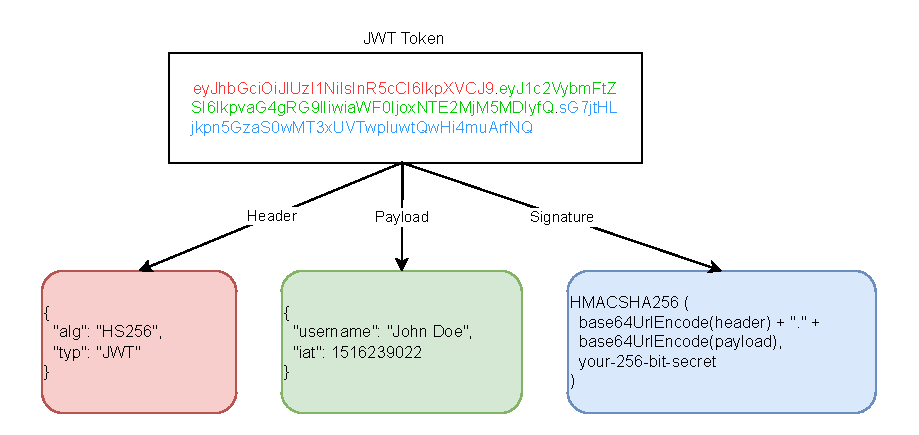
\includegraphics[width=1.1\columnwidth]{graphics/jwt-explained.pdf}
		\caption{Detailed explanation of JWT-based authentication mechanism.}
		\label{fig:jwt-explained}
	\end{figure}
	
	
		\vspace*{0.5cm}
	\begin{tabular}{ @{} m{0.25\textwidth} m{0.7\textwidth} @{} }
		\begin{minipage}{\linewidth}
			\centering
			
\includegraphics[width=0.5\linewidth]{graphics/redis.png}
			\captionof{figure}{Redis Logo}
			\label{fig:redis}
		\end{minipage}
		&
		\begin{minipage}{\linewidth}
			\textbf{Redis} is an in-memory data structure store, commonly used as a database, cache, and message broker. It is part of the NoSQL database category called key/value stores. Keys serve as unique identifiers, and their corresponding values can be any of the data types supported by Redis. These data types include basic Strings, Linked Lists, Sets, and Streams, each with its own specific behaviors and commands. \cite{redis-what-is} In this system, Redis is specifically utilized for session management, particularly in storing refresh tokens. By caching these tokens, Redis helps to reduce the load on the primary database, which improves both scalability and performance. Since Redis operates in memory, it allows for faster retrieval of session data, ensuring that the authentication process remains responsive and efficient. Additionally, Redis offers built-in features like automatic expiration, which helps in managing token lifetimes and ensuring secure token invalidation, further enhancing the security and reliability of the system.
		\end{minipage}
	\end{tabular}
	
	
	
	\subsubsection{Database: PostgreSQL}
	
	\begin{figure}[H]
		\centering
		
\includegraphics[scale=0.1]{graphics/postgresql.png}
		\caption{PostgreSQL \acs{rdbms} Logo}
		\label{fig:postgresql}
	\end{figure}
	
	PostgreSQL is a powerful, open-source relational database that provides strong ACID (Atomicity, Consistency, Isolation, Durability) compliance, ensuring reliability and data integrity, which is critical for managing sensitive information such as user accounts, ticketing systems, and communication logs. Its robust support for advanced querying and indexing mechanisms ensures that the system can handle complex searches and queries with high efficiency, even as data grows over time. \cite{postgres}\\
	
	PostgreSQL also supports features like foreign key constraints, triggers, and stored procedures, which help in maintaining data consistency across multiple tables, ensuring that relationships between different data entities (such as users and tickets) are enforced and managed correctly. Additionally, its ability to support JSON and JSONB data types allows the system to store and query semi-structured data, offering flexibility in handling modern web applications that require both structured and unstructured data. \\
	
	The database also scales well, supporting a large number of concurrent users and high-volume transactions, making it an ideal choice for applications with growing user bases. PostgreSQL’s support for full-text search and geospatial data (via PostGIS) can be useful for implementing advanced search functionalities and geographical features in the system. With its extensibility (allowing the addition of custom functions, data types, and more), PostgreSQL provides a solid and scalable foundation for the back-end data management of the system. \\
	
	\subsubsection{Responsive Web Design: Techniques and Tools}
	
	\begin{itemize}
		\item \textbf{Media Queries}: CSS media queries are used to apply different styles based on device characteristics (screen size, resolution). This allows the frontend to automatically adapt to different devices, ensuring that the system is usable on desktops, laptops, tablets, and smartphones.
		
		\item \textbf{CSS Flexbox/Grid}: These CSS layout models allow for flexible, responsive layouts that adjust to different screen sizes. Flexbox is ideal for managing component positioning in small screens, while Grid is useful for creating complex layouts in larger screens.
	\end{itemize}


\subsection{Theoretical Background}

	\subsubsection{Ticket Management Systems}
	A ticket management system is a tool designed to manage and track the progress of support requests, from the time they are submitted until they are resolved. The system typically assigns a unique identifier (ticket) to each request, enabling staff to monitor progress, prioritize issues, and provide timely responses.
	In a university context, ticket management systems are particularly useful for handling student issues, such as dormitory problems, academic inquiries, and administrative requests. By assigning specific staff members to tickets, the system ensures accountability and reduces response time.
	
	\subsubsection{Real-Time Communication Tools}
	Real-time communication tools like SocketIO or WebSockets are essential in modern web applications. These tools allow for instantaneous data transmission between the server and client, enabling real-time messaging and live updates. For instance, in the Student Life Support Service, students and staff can exchange messages directly without having to refresh the page, ensuring efficient communication.
	
	\subsubsection{Web Application Development Best Practices}
	\begin{itemize}
		\item \textbf{Modular Design}: Applications should be developed in a modular fashion, separating concerns into distinct components (frontend, backend, database). This allows for easier maintenance and scalability.
		
		\item \textbf{Security First}: With the increasing number of security breaches in web applications, implementing security best practices like JWT for authentication, HTTPS for communication, and proper data validation is essential.
		
		\item \textbf{Responsive Design}: Ensuring that the application works across different devices and screen sizes is a fundamental best practice, especially for a university setting where students and staff might use a wide variety of devices.
	\end{itemize}
		
		
\subsection{Gap Analysis}

	\subsubsection{What is Missing from Existing Solutions}
	Existing solutions for university support systems face several shortcomings. Privacy concerns arise in social media-based group chats, where sensitive student information may be exposed, and even proprietary systems lack a strong focus on educational privacy needs. Role-specific functionalities are often missing, with few systems offering specialized tools for students, dormitory staff, or administrators, or including student-centric features like feedback collection, ticket rating, and public status views. Limited analytics is another issue; while general analytics are provided, they don’t cater to the specific needs of student services, such as tracking recurring issues or ticket performance. Additionally, many systems, like JIRA, are not user-friendly for students, requiring training and posing barriers in environments where simplicity is essential.
	
	\subsubsection{How the Student Life Support Service Fills These Gaps}
	The Student Life Support Service addresses the gaps in existing systems by offering a solution tailored specifically to university needs. Its customizable structure supports role-specific functionalities for students, dormitory staff, and administrators, making it ideal for managing university-specific scenarios like dormitory issues and academic inquiries. Real-time communication is enabled through SocketIO, allowing fast, interactive responses between students and staff. The user-friendly interface, built with ReactJS and Material UI, ensures easy navigation for non-technical users. As an open-source, cost-effective platform using NodeJS, PostgreSQL, and ReactJS, it avoids the high costs of proprietary software. The system also provides role-specific features, such as ticket creation, tracking, and rating for students, efficient ticket handling for staff, and detailed reporting tools for administrators. Enhanced privacy and security are ensured through JWT-based authentication and role-based access, preventing unauthorized access to sensitive information. Additionally, built-in data analytics offers administrators insights into ticket trends and areas for improvement in student support services.
	
	
	
	
	
			
\section{System Design}

\subsection{Functional Requirements}
The Student Life Support Service is designed to fulfill the specific functional requirements of three key user roles: Students, Dormitory Staff (or Student Affairs), and Administrators. Each role has its own set of features tailored to its needs within the system.

\noindent \textbf{User Type}: S-Student, DS-Dormitory Staff/Student Affairs, A-Admin (Operator) \\
\textbf{Categorized}: F-Functional, NF-Nonfunctional

\newcolumntype{L}{>{\arraybackslash}m{3.5cm}}
\begin{longtable}{|m{0.6cm}|m{2.8cm}|m{5.4cm}|m{1.6cm}|m{1.5cm}|m{1.8cm}|}
	\hline
	\textbf{No} & \textbf{Requirement }             & \textbf{Description}                                                                                          & \textbf{Priority} & \textbf{User Type}  & \textbf{Category} \\ \hline
	\endhead
	1  & Manage personal info     & Users can view and update their personal information.                                                 & Medium   & S, DS, A   & F           \\ \hline
	2  & Support tickets          & Users can create (raise), view support tickets.                                                       & High     & S, DS, A   & F           \\ \hline
	3  & Contact through messages & Users can contact the staff or students handling the support ticket through text messages.            & High     & S, DS      & F           \\ \hline
	4  & Ticket rating            & Students can rate their tickets which are marked as done.                                             & Medium   & S          & F           \\ \hline
	5  & View newsfeed            & Users can view a newsfeed of public pending/in-process tickets.                                        & Low      & S, DS, A   & F           \\ \hline
	6  & View notifications       & Users can view notifications and announcements.                                                       & Medium   & S, DS, A   & F           \\ \hline
	7  & Feedback and suggestions & Users can give feedback and suggestions for the system.                                                & Medium   & S, DS, A   & F          \\ \hline
	8  & Handle support tickets   & Dormitory staff can view and handle (mark as done, cancel) support tickets.                            & High     & DS         & F           \\ \hline
	9  & View past tickets        & Dormitory staff can view all previously handled support tickets.                                       & Medium   & DS         & F           \\ \hline
	10 & Manage notifications     & Dormitory staff and admins can create and manage notifications and announcements.                      & High     & DS, A      & F           \\ \hline
	11 & Manage users             & Admins can manage all users/roles (create, view, update, delete).                                      & High     & A          & F           \\ \hline
	12 & Manage tickets           & Admins can manage all support tickets (view, delete).                                                  & High     & A          & F           \\ \hline
	13 & Manage dormitories       & Admins can manage all dormitories (create, view, delete).                                              & Medium   & A          & F           \\ \hline
	14 & Manage system logs       & Admins can manage system logs (view, delete).                                                          & Medium   & A          & F           \\ \hline
	15 & Manage feedback          & Admins can manage system feedback (view, delete).                                                      & Low      & A          & F           \\ \hline
	16 & View system report       & Admins can generate and view system reports.                                                           & High     & A          & F           \\ \hline
	
	
	\caption{Functional Requirements}
	\label{tab:functionalRequirement}
\end{longtable}


For clearer comprehension, the table presented below provides a detailed visualization of the functional requirements, organized according to the different user roles within the system. This structure allows for a more precise understanding of how each role interacts with the system's features and capabilities.

\begin{longtable}{{|m{4.8cm}|m{12cm}|}} 
	\hline
	\textbf{User roles} & \textbf{Functional Requirements}\\ \hline
	\endhead
	
	Student & 	
	\begin{itemize}
		\item can view, update his/her personal information.
		\item can create (raise), view his/her support tickets. 
		\item can contact the staff who handles the support ticket through text messages.
		\item can rate his/her tickets which are marked as done.
		\item can view newsfeed (public pending/in process tickets).
		\item can view notifications, announcement.
		\item can give feedback and suggestions for the system.
	\end{itemize}
	
	\\ \hline
	
	Dormitory staff/ Student Affairs & 	
	\begin{itemize}
		\item can view, update his/her personal information.
		\item can view all available support tickets.
		\item can handle support tickets. (mark as done, cancelled)
		\item can view all past handled tickets.
		\item can contact students who owns the ticket through text messages.
		\item can view newsfeed (public pending/in process tickets).
		\item can create, view notifications, announcement. 
		\item can give feedback and suggestions for the system.
	\end{itemize}
	
	\\ \hline
	
	
	Admin (Operator) & 	
	\begin{itemize}
		\item can manage his/her personal information (view, update).
		\item can manage all users/roles (create, view, update, delete).
		\item can manage all support tickets (view, delete).
		\item can manage all dormitories (create, view, delete).
		\item can manage system logs (view, delete).
		\item can manage system feedback (view, delete).
		\item can view newsfeed (public pending/in process tickets).
		\item can manage notifications, announcement (create, view). 
		\item can view the system report.
	\end{itemize}
	
	\\ \hline
	
	
	\caption{Functional Requirements by User Roles} % needs to go inside longtable environment
	\label{tab:functionalRequirements}
\end{longtable}



\subsection{Non-Functional Requirements}
\noindent \textbf{Categorized}: NF-Nonfunctional

\newcolumntype{L}{>{\arraybackslash}m{3.5cm}}



	\begin{longtable}{|m{0.5cm}|m{2.5cm}|m{7cm}|m{1.5cm}|m{1.7cm}|m{2.4cm}|}
		\hline
		\textbf{No} & \textbf{Requirement}                & \textbf{Description}                                                                                                                               & \textbf{Priority} & \textbf{Category}  & \textbf{Functioning} \\ \hline
		\endhead
		1  & Fast Response Time          & The system should provide fast responses for user interactions such as submitting tickets, viewing statuses, and real-time messaging.      & High     & NF        & Performance \\ \hline
		2  & Real-Time Communication     & Messages between students and staff should be transmitted with minimal latency (under 100 milliseconds).                                   & High     & NF        & Performance \\ \hline
		3  & Concurrent Users            & The system must support up to 500 concurrent users without significant performance degradation.                                            & High     & NF        & Performance \\ \hline
		4  & Database Query Optimization & PostgreSQL database should be optimized to handle high read/write volume efficiently even during peak load.                                & High     & NF        & Performance \\ \hline
		5  & JWT-Based Authentication    & Secure authentication using JSON Web Tokens (JWT), with short-lived tokens and securely stored refresh tokens in Redis.                    & High     & NF        & Security    \\ \hline
		6  & Role-Based Access Control   & Enforce strict role-based access to ensure users only have access to the functionality appropriate for their role.                         & High     & NF        & Security    \\ \hline
		7  & Encryption                  & All communications between the client and server must be encrypted using HTTPS to ensure data security.                                    & High     & NF        & Security    \\ \hline
		8  & Data Validation             & Input from users must be validated and sanitized to protect against common vulnerabilities like SQL Injection and Cross-Site Scripting.     & High     & NF        & Security    \\ \hline
		9  & Audit Logs                  & Admins must have access to immutable and secure audit logs to track user actions such as login attempts and system modifications.           & Medium   & NF        & Security    \\ \hline
		10 & Database Scalability        & The PostgreSQL database should scale efficiently as the number of tickets, messages, and users grows.                                       & High     & NF        & Scalability \\ \hline
		11 & User-Friendly Interface     & The interface should be intuitive and easy to navigate for users of varying technical abilities.                                            & High     & NF        & Usability   \\ \hline
		12 & Cross-Device Compatibility  & The system should be responsive and function well on desktops, laptops, tablets, and smartphones.                                           & High     & NF        & Usability   \\ \hline
	
		\caption{Non-Functional Requirements}
	\label{tab:nonfunctionalRequirements}
	
	\end{longtable}



\subsection{Use Case Diagrams}
	\begin{figure}[H]
		\centering
		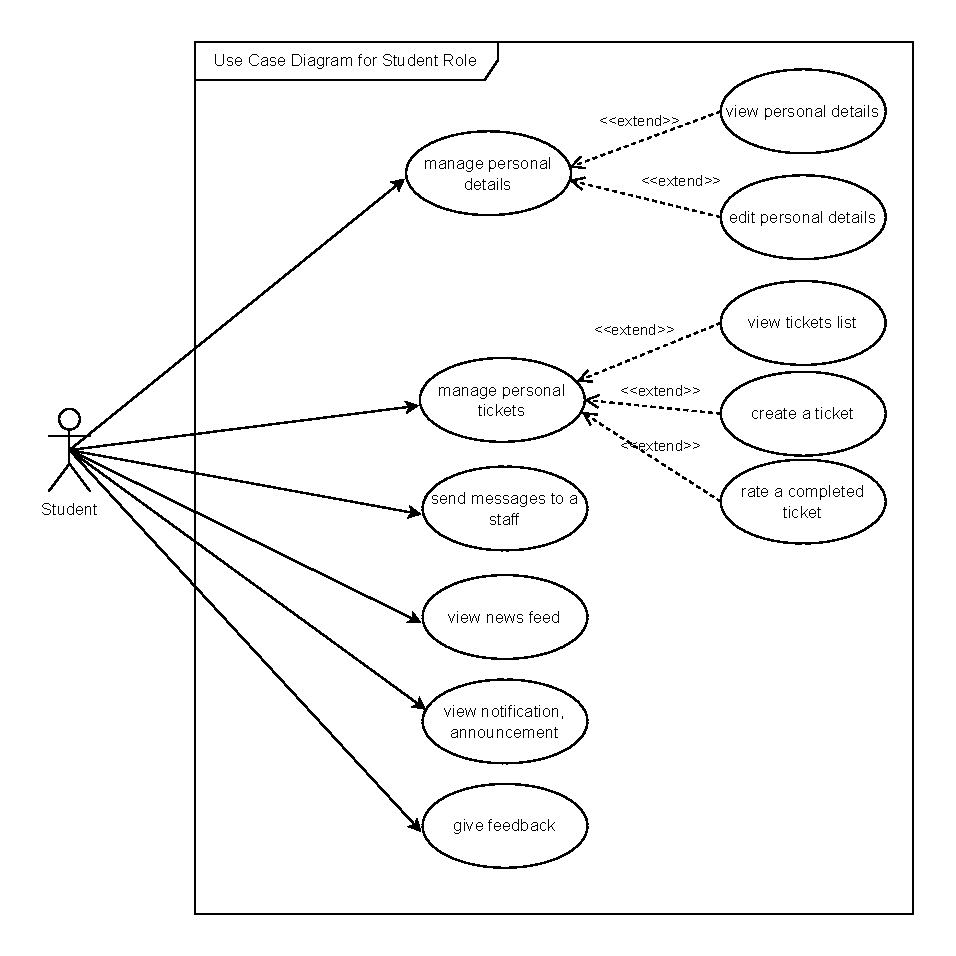
\includegraphics[width=0.82\columnwidth]{graphics/student use case.pdf}
		\caption{Student Use Case Diagram}
		\label{fig:student-use-case}
	\end{figure}
	
	
	
	\begin{figure}[H]
		\centering
		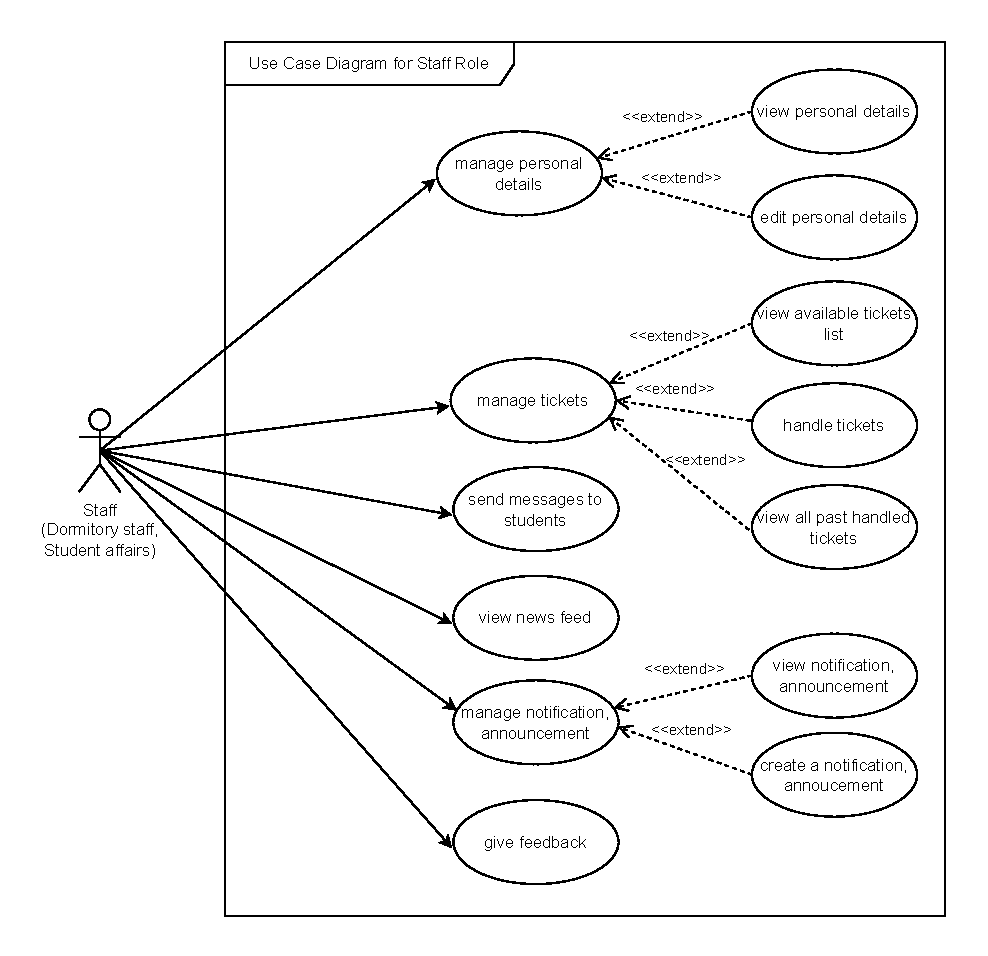
\includegraphics[width=0.9\columnwidth]{graphics/staff use case.pdf}
		\caption{Staff (Dormitory staff, Student affairs) Use Case Diagram}
		\label{fig:staff-use-case}
	\end{figure}
	
	
	
	\begin{figure}[H]
		\centering
		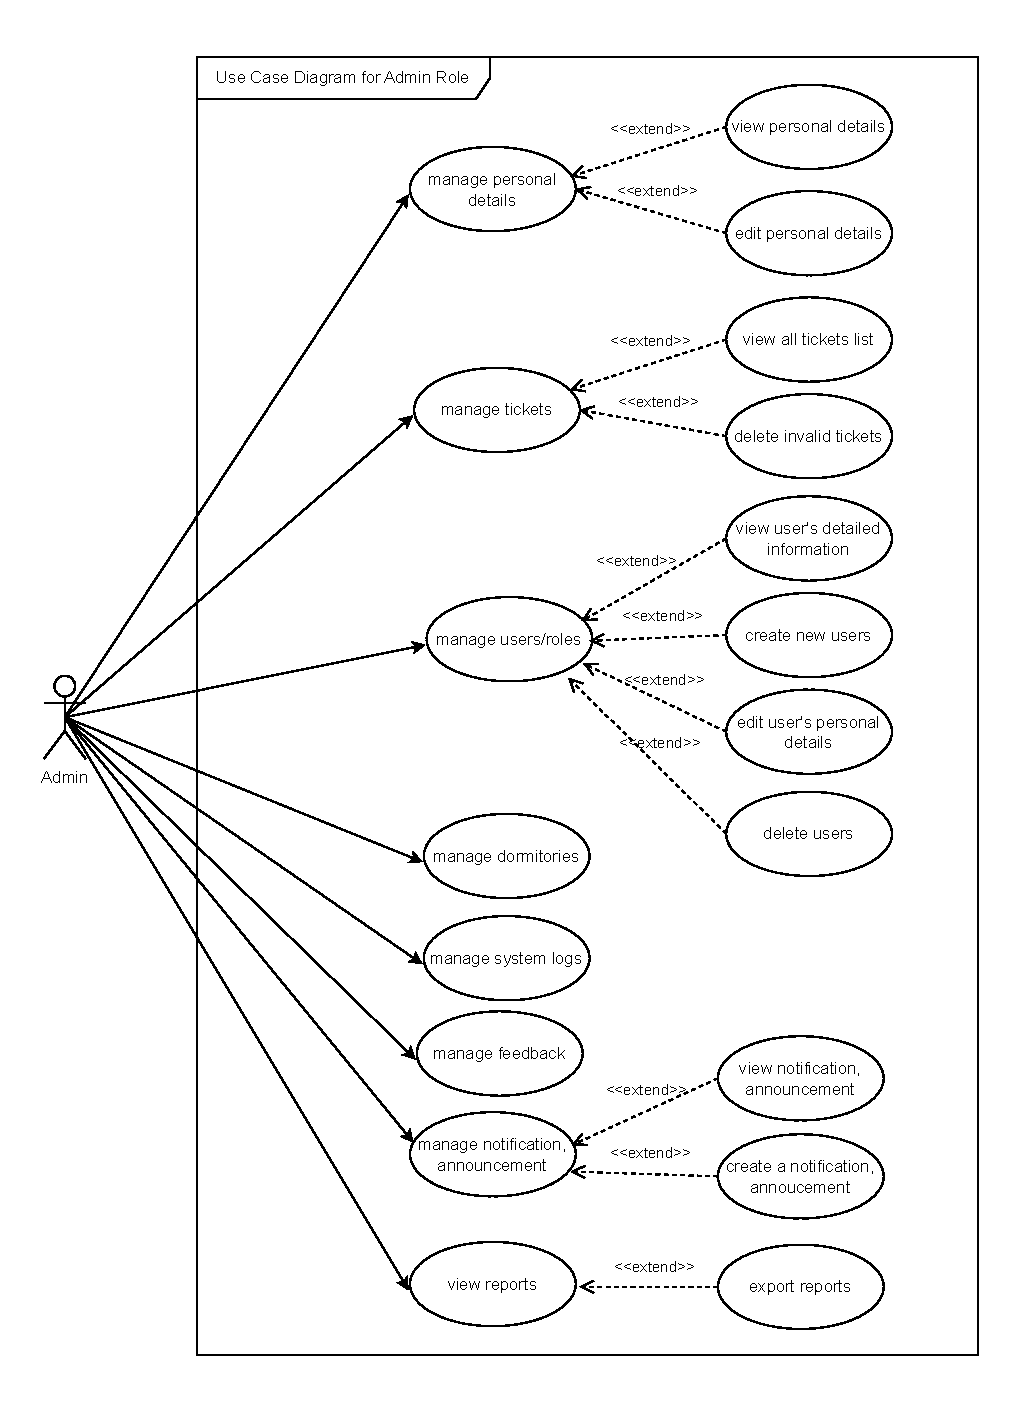
\includegraphics[width=0.84\columnwidth]{graphics/admin-use-case.pdf}
		\caption{Admin Use Case Diagram}
		\label{fig:admin-use-case}
	\end{figure}
	
	
\subsection{Process Workflow Diagrams}	
The core functionality of the Student Life Support Service is its ticket-raising process. The following diagram provides a detailed step-by-step illustration of this process.


\begin{figure}[H]
	\centering
	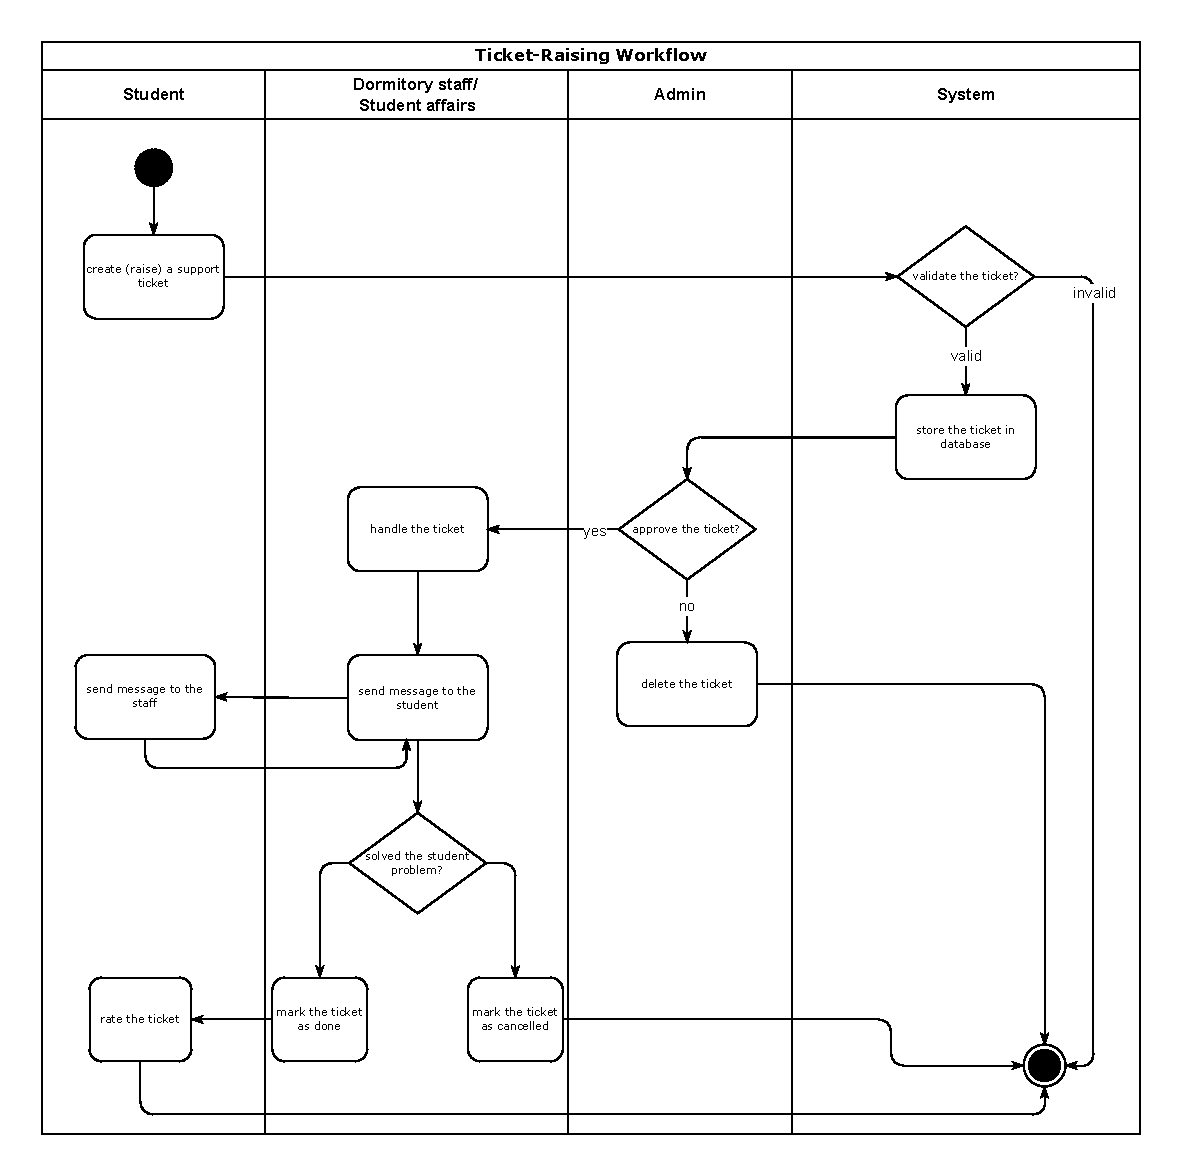
\includegraphics[width=1\columnwidth]{graphics/sys-workflow.pdf}
	\caption{Ticket-Raising Process Workflow}
	\label{fig:ticket-raising-workflow}
\end{figure}


\subsection{Database Design}
	\subsubsection{ER Diagram}
	\begin{figure}[H]
		\centering
		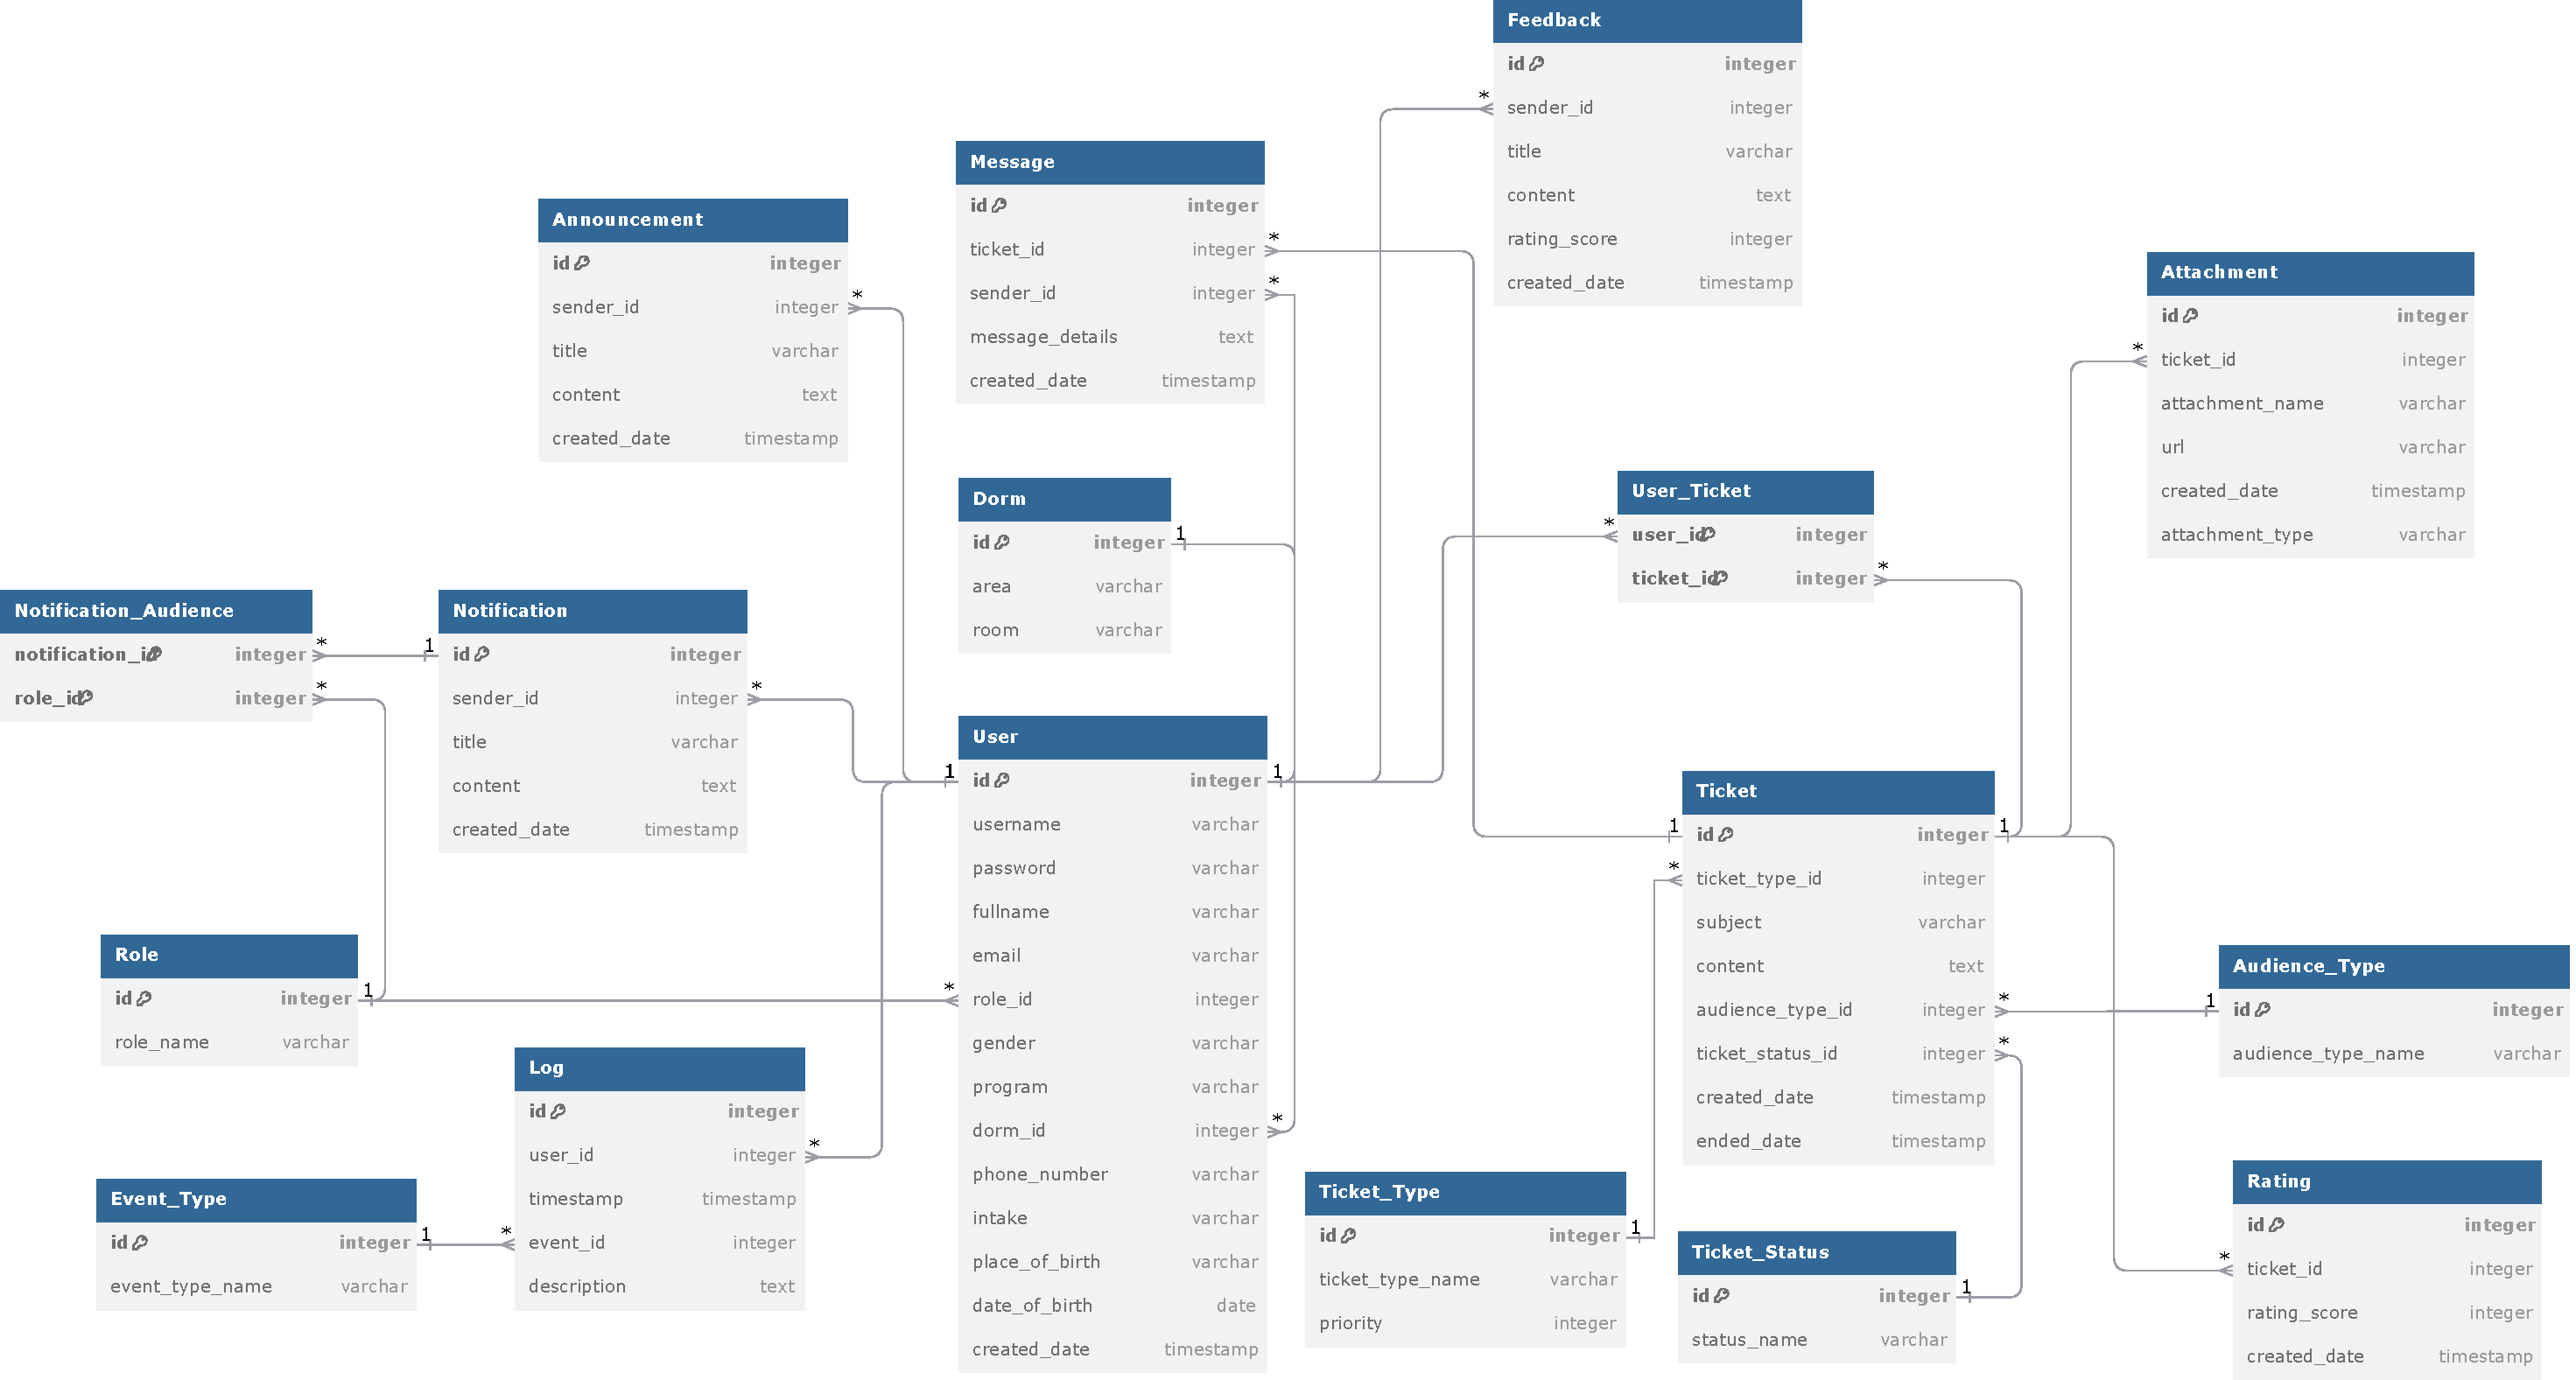
\includegraphics[width=1 \columnwidth]{graphics/er-diagram-v2.pdf}
		\caption{ER Diagram}
		\label{fig:er-diagram}
	\end{figure}


	\subsubsection{User Entity}
%	\newcolumntype{L}{>{\arraybackslash}m{3.5cm}}
	The User entity is fundamental to the system's user management, encompassing essential information that defines each user’s profile and access rights. This entity includes several key attributes that contribute to its operational integrity (see Table \ref{tab:user-entity})
	
	
	
	\begin{longtable}{|m{1.4cm}|m{2.8cm}|m{2.3cm}|m{2.3cm}|m{7.2cm}|}
		\hline
		\textbf{Key Type} & \textbf{Field Name} & \textbf{Data Type}                                                                                                                            & \textbf{Constraints} & \textbf{Description}   \\ \hline
		\endhead
		
		Primary & id & serial (int) & \makecell[l]{NOT NULL} & id of a user \\ \hline
		 & username & varchar(255) & \makecell[l]{NOT NULL \\ UNIQUE} & the user name of a user, it could be matriculation number of a student \\ \hline
		 & email & varchar(255) & \makecell[l]{NOT NULL \\ UNIQUE} & the email of a user \\ \hline
		 & fullname & varchar(255) & \makecell[l]{NOT NULL} & the full name of a user \\ \hline
		 & gender & varchar(255) & \makecell[l]{NOT NULL} & the gender of a user \\ \hline
		 Foreign & role\_id & int & \makecell[l]{NOT NULL} & the role id of a user \\ \hline
		 Foreign & dorm\_id & int & \makecell[l]{NOT NULL} & the dorm id where user lives (if the user does not live in a dormitory, dorm\_id value equals to 1)\\ \hline
		 & program & varchar(255) &  & the program that user registered at university (E.g: Computer Science, Architecture, etc.)\\ \hline
		 & intake & varchar(255) &  & the time when a user registered a specific program at university (E.g: 2020, 2021, etc.)\\ \hline
		 & phone\_number & varchar(255) & \makecell[l]{NOT NULL} & the phone number of a user\\ \hline
		 & place\_of\_birth & varchar(255) & \makecell[l]{NOT NULL} & the birth place of a user\\ \hline
		 & date\_of\_birth & date & \makecell[l]{NOT NULL} & the birth date of a user\\ \hline
		 & password & varchar(255) & \makecell[l]{NOT NULL} & the password of a user (in hashed string) \\ \hline
		 & created\_date & \makecell[l]{timestamp \\with time \\zone} & NOT NULL & the date time when a user account is created in the system \\ \hline
		 
		
		\caption{User Entity}
		\label{tab:user-entity}
		
	\end{longtable}
	
	
	
	
	\subsubsection{Ticket Entity}
	This table outlines the key attributes necessary for managing ticket entities within the system. It includes various fields such as the ticket ID, type, subject, content, and associated status. Additionally, it specifies data types, constraints, and a detailed description of each field to ensure proper handling of ticket information (refer to Table \ref{tab:ticket-entity}).
	
	
	
	\begin{longtable}{|m{1.4cm}|m{3.3cm}|m{2.3cm}|m{2.3cm}|m{6.7cm}|}
		\hline
		\textbf{Key Type} & \textbf{Field Name} & \textbf{Data Type}                                                                                                                            & \textbf{Constraints} & \textbf{Description}   \\ \hline
		\endhead
		
		Primary & id & serial (int) & \makecell[l]{NOT NULL} & id of a ticket \\ \hline
		Foreign & ticket\_type\_id & int & \makecell[l]{NOT NULL} & the id of the ticket type \\ \hline
		 & subject & varchar(255) & \makecell[l]{NOT NULL} & the subject (title) the ticket \\ \hline
		 & content & text & \makecell[l]{NOT NULL} & the detailed description of the problem declared in the ticket \\ \hline
		Foreign & audience\_type\_id & int & \makecell[l]{NOT NULL} & the id of audience type assigned to the ticket \\ \hline
		Foreign & ticket\_status\_id & int & \makecell[l]{NOT NULL} & the id of current status assigned to the ticket \\ \hline
		& created\_date & \makecell[l]{timestamp \\with time \\zone} & NOT NULL & the date time when a ticket is created in the system \\ \hline
		& ended\_date & \makecell[l]{timestamp \\with time \\zone} & NOT NULL & the date time when a ticket is marked as done or cancelled in the system \\ \hline
		
		
		\caption{Ticket Entity}
		\label{tab:ticket-entity}
		
	\end{longtable}
	
	
	\subsubsection{User\_Ticket Relationship}
	
		\begin{longtable}{|m{1.4cm}|m{3.3cm}|m{2.3cm}|m{2.3cm}|m{6.7cm}|}
			\hline
			\textbf{Key Type} & \textbf{Field Name} & \textbf{Data Type}                                                                                                                            & \textbf{Constraints} & \textbf{Description}   \\ \hline
			\endhead
			
			Primary & user\_id & int & \makecell[l]{NOT NULL} & id of a ticket \\ \hline
			
			Primary & ticket\_id & int & \makecell[l]{NOT NULL} & id of a user \\ \hline

			\caption{User\_Ticket Relationship}
			\label{tab:user-ticket}
			
		\end{longtable}
		
		This table describes the relationship between users and tickets within the system. It contains two primary key fields: \texttt{user\_id} and \texttt{ticket\_id}, each identified by a unique integer. The \texttt{user\_id} represents the unique identifier for a user, while the \texttt{ticket\_id} corresponds to a unique ticket within the system. Both fields are non-nullable, ensuring that each user and ticket association is properly recorded and maintained (refer to Table \ref{tab:user-ticket}). This relationship is essential for tracking which users have raised and handled specific tickets in the system .
	
	
	\subsubsection{Ticket\_Type Entity}
	The Ticket\_Type entity serves to classify different categories of tickets within the system, each defined by a unique identifier and a descriptive name. It also includes a priority level that indicates the urgency of each ticket type, where a higher value corresponds to a lower priority. This structure enables efficient ticket management and prioritization (see Table \ref{tab:ticket-type}).
	
	\begin{longtable}{|m{1.4cm}|m{3.3cm}|m{2.3cm}|m{2.3cm}|m{6.7cm}|}
		\hline
		\textbf{Key Type} & \textbf{Field Name} & \textbf{Data Type}                                                                                                                            & \textbf{Constraints} & \textbf{Description}   \\ \hline
		\endhead
		
		Primary & id & serial (int) & \makecell[l]{NOT NULL} & id of a ticket type \\ \hline
		 & ticket\_type\_name & varchar(255) & \makecell[l]{NOT NULL \\ UNIQUE} & the type name of a ticket \\ \hline
		
		& priority & int & \makecell[l]{NOT NULL} & the priority of the ticket type (higher indicates lower priority) \\ \hline
		
		\caption{Ticket\_Type Entity}
		\label{tab:ticket-type}
		
	\end{longtable}
	
%	This table defines the Ticket\_Type entity, which represents various types of tickets that can be created within the system. It consists of three fields:
%
%	\begin{itemize}
%		\item The \texttt{id} field, which is a primary key, represented as a serial integer, serving as the unique identifier for each ticket type.
%		
%		\item The \texttt{ticket\_type\_name} field, stored as a \texttt{varchar(255)}, holds the name of the ticket type, such as "Lost items" or "Harassment".
%		
%		\item The \texttt{priority} field, an integer, determines the urgency level of the ticket type, where a higher number indicates lower priority.
%	\end{itemize}
%	
%	\noindent All fields are marked as \texttt{NOT NULL}, ensuring that every ticket type has a unique identifier, name, and priority level. This structure is essential for organizing and managing different categories of support tickets in the system (refer to Table \ref{tab:ticket-type}).
	
	
	
	\subsubsection{Ticket\_Status Entity}
	The Ticket\_Status entity is designed to define various states that a ticket can be in within the system. Each status is uniquely identified by an ID and has a descriptive name, allowing for clear tracking and management of tickets throughout their lifecycle. This structured approach enhances the ability to monitor ticket progress and provides clarity to users regarding the current status of their tickets (see Table \ref{tab:ticket-status}).
	
	\begin{longtable}{|m{1.4cm}|m{3.3cm}|m{2.3cm}|m{2.3cm}|m{6.7cm}|}
		\hline
		\textbf{Key Type} & \textbf{Field Name} & \textbf{Data Type}                                                                                                                            & \textbf{Constraints} & \textbf{Description}   \\ \hline
		\endhead
		
		Primary & id & serial (int) & \makecell[l]{NOT NULL} & id of a ticket status \\ \hline
		& status\_name & varchar(255) & \makecell[l]{NOT NULL \\ UNIQUE} & the status name of a ticket \\ \hline
		
		\caption{Ticket\_Status Entity}
		\label{tab:ticket-status}
		
	\end{longtable}
	
	
%	This table describes the Ticket\_Status entity, which is used to represent the current status of a support ticket within the system. It contains two fields:
%	
%	
%	\begin{enumerate}
%		
%		\item The \texttt{id} field is the primary key, defined as a serial integer, serving as the unique identifier for each ticket status. This field is essential for distinguishing between different statuses.
%		
%		\item The \texttt{status\_name} field is a \texttt{varchar(255)} that stores the name of the ticket status, such as "pending," "in progress," "done," or "cancelled." These status names provide insight into the progress of each support ticket.
%	\end{enumerate}
%	
%	\noindent Both fields are marked as \texttt{NOT NULL}, ensuring that every ticket status has a unique identifier and name, which is crucial for tracking and managing the lifecycle of tickets (refer to Table \ref{tab:ticket-status}).
	
	
	
	\subsubsection{Audience\_Type Entity}
	
	The Audience\_Type entity categorizes target audiences for tickets in the system. Each type is uniquely identified by an ID and has a descriptive name, enhancing communication and ticket management for specific user groups (see Table \ref{tab:audience-type}).
	
	\begin{longtable}{|m{1.4cm}|m{3.8cm}|m{2.3cm}|m{2.3cm}|m{6.2cm}|}
		\hline
		\textbf{Key Type} & \textbf{Field Name} & \textbf{Data Type}                                                                                                                            & \textbf{Constraints} & \textbf{Description}   \\ \hline
		\endhead
		
		Primary & id & serial (int) & \makecell[l]{NOT NULL} & id of a ticket audience type \\ \hline
		& audience\_type\_name & varchar(255) & \makecell[l]{NOT NULL \\ UNIQUE} & the target audience type name of a ticket \\ \hline
		
		\caption{Audience\_Type Entity}
		\label{tab:audience-type}
		
	\end{longtable}
	
	
%	This table outlines the Audience\_Type entity, which is used to categorize the audience for support tickets within the system. It includes two fields:
%	
%	\begin{itemize}
%		\item The \texttt{id} field, which is the primary key, is a serial integer that uniquely identifies each audience type. This field ensures each audience type is distinct and traceable.
%		
%		\item The \texttt{audience\_type\_name} field is a \texttt{varchar(255)} that stores the name of the audience type for a ticket. It could be either "private" or "public," where public tickets are visible to other students, while private tickets are only visible to the ticket creator and assigned staff.
%	\end{itemize}
%	
%
%	\noindent Both fields are defined as NOT NULL, ensuring that each audience type has a unique identifier and a clearly defined type name, which is essential for managing ticket visibility (refer to Table \ref{tab:audience-type}).
%	
	
	
	\subsubsection{Attachment Entity}
	The Attachment entity manages files associated with tickets in the system. Each attachment is uniquely identified by an ID and linked to a specific ticket through a foreign key. The entity includes attributes for the original file name, its server \acs{url}, and the timestamp of its upload, ensuring organized storage and retrieval of related documents for user reference (see Table \ref{tab:attachment}).
	
	\begin{longtable}{|m{1.4cm}|m{3.3cm}|m{2.3cm}|m{2.3cm}|m{6.3cm}|}
		\hline
		\textbf{Key Type} & \textbf{Field Name} & \textbf{Data Type}                                                                                                                            & \textbf{Constraints} & \textbf{Description}   \\ \hline
		\endhead
		
		Primary & id & serial (int) & \makecell[l]{NOT NULL} & id of an attachment \\ \hline
		Foreign & ticket\_id & int & \makecell[l]{NOT NULL} & the reference ticket id which has an attachment \\ \hline
		 & attachment\_name & varchar(255) & \makecell[l]{NOT NULL} & the original name of the attachment \\ \hline
		 & url & varchar(255) & \makecell[l]{NOT NULL \\ UNIQUE} & the address of an attachment on the server  \\ \hline
		 & created\_date & \makecell[l]{timestamp \\with time \\zone} & NOT NULL & the date time when an attachment is firstly uploaded to the system \\ \hline
		
		\caption{Attachment Entity}
		\label{tab:attachment}
		
	\end{longtable}
	
%	The Attachment entity captures essential details about files associated with support tickets in the system. The table comprises the following key fields:
%	
%	\begin{itemize}
%		\item \texttt{id}: This primary key is a serial integer that uniquely identifies each attachment in the system, ensuring every file is traceable.
%		
%		\item \texttt{ticket\_id}: A foreign key linking the attachment to the specific ticket it belongs to, creating a clear relationship between files and their corresponding support tickets.
%		
%		\item \texttt{attachment\_name}: This field stores the original name of the file, providing users and administrators with a clear reference to the document.
%		
%		\item \texttt{url}: A \texttt{varchar(255)} field that holds the unique server address where the attachment is stored. It is constrained to be both \texttt{NOT NULL} and \texttt{UNIQUE}, ensuring each file is stored at a distinct location.
%		
%		\item \texttt{created\_date}: A timestamp with time zone that records the exact moment the attachment was uploaded to the system, offering important chronological information for ticket management.
%	\end{itemize}
%
%	\noindent This entity provides a robust structure for managing files, enabling easy access and secure storage of attachments related to user support requests (refer to Table \ref{tab:attachment}).
	
	
	
	\subsubsection{Rating Entity}
	The Rating entity captures user ratings for tickets in the system. Each rating is uniquely identified by an ID and linked to a specific ticket through a foreign key. It includes a score reflecting the user's assessment and a timestamp indicating when the rating was given, enabling effective tracking of user feedback (see Table \ref{tab:rating}).
	
	\begin{longtable}{|m{1.4cm}|m{2.5cm}|m{2.3cm}|m{2.3cm}|m{6.7cm}|}
		\hline
		\textbf{Key Type} & \textbf{Field Name} & \textbf{Data Type}                                                                                                                            & \textbf{Constraints} & \textbf{Description}   \\ \hline
		\endhead
		
		Primary & id & serial (int) & \makecell[l]{NOT NULL} & id of a rating \\ \hline
		Foreign & ticket\_id & int & \makecell[l]{NOT NULL} & the reference ticket id which has the rating \\ \hline
		& rating\_score & int & \makecell[l]{NOT NULL} & the rating score of a ticket \\ \hline
		& created\_date & \makecell[l]{timestamp \\with time \\zone} & NOT NULL & the date time when user rates a ticket. \\ \hline
		
		\caption{Rating Entity}
		\label{tab:rating}
		
	\end{longtable}
	
%	The Rating entity is designed to capture and store feedback from users regarding their support tickets. This table includes several key fields:
%	
%	\begin{itemize}
%		\item \texttt{id}: A serial integer serving as the primary key, which uniquely identifies each rating entry in the system.
%		
%		\item \texttt{ticket\_id}: A foreign key that links the rating to the specific ticket being evaluated, ensuring that every rating is associated with a particular support request.
%		
%		\item \texttt{rating\_score}: A number field that holds the actual score or feedback provided by the user. This score reflects the user's level of satisfaction with the handling of their ticket.
%		
%		\item \texttt{created\_date}: A timestamp with time zone indicating when the rating was submitted, allowing for tracking and auditing of feedback over time.
%	\end{itemize}
%	
%	\noindent This entity is crucial for maintaining a structured and traceable system for user feedback, enabling continuous service improvement based on user satisfaction (refer to Table \ref{tab:rating}).
	
	
	
	\subsubsection{Feedback Entity}
	
	The Feedback entity collects user feedback on various aspects of the system. Each feedback entry is uniquely identified by an ID and linked to the user providing it through a foreign key. It includes a title for the feedback, detailed content, a rating score reflecting the user's evaluation, and a timestamp indicating when the feedback was submitted. This structure facilitates the collection and analysis of user opinions to enhance system performance (see Table \ref{tab:feedback}).
	
	\begin{longtable}{|m{1.4cm}|m{2.5cm}|m{2.3cm}|m{2.3cm}|m{6.7cm}|}
		\hline
		\textbf{Key Type} & \textbf{Field Name} & \textbf{Data Type}                                                                                                                            & \textbf{Constraints} & \textbf{Description}   \\ \hline
		\endhead
		
		Primary & id & serial (int) & \makecell[l]{NOT NULL} & id of a feedback \\ \hline
		Foreign & sender\_id & int & \makecell[l]{NOT NULL} & the id of the user who gives the feedback \\ \hline
		& title & varchar(255) & \makecell[l]{NOT NULL} & the title (subject) of the feedback \\ \hline
		& content & text & \makecell[l]{NOT NULL} & the details of the feedback \\ \hline
		& rating\_score & int & \makecell[l]{NOT NULL} & the rating score of the feedback \\ \hline
		& created\_date & \makecell[l]{timestamp \\with time \\zone} & NOT NULL & the date time when user gives the feedback. \\ \hline
		
		\caption{Feedback Entity}
		\label{tab:feedback}
		
	\end{longtable}
%	
%	The Feedback entity is structured to store user feedback, enabling users to provide detailed evaluations of the system. It consists of several key fields:
%	
%	\begin{itemize}
%		\item \texttt{id}: A serial integer that serves as the primary key, uniquely identifying each feedback entry.
%		
%		\item \texttt{sender\_id}: A foreign key representing the user who submits the feedback, ensuring proper linkage between the feedback and its author.
%		
%		\item \texttt{title}: A \texttt{varchar(255)} field that contains the subject or title of the feedback, summarizing the main point of the user's input.
%		
%		\item \texttt{content}: A text field used for the detailed explanation of the feedback, where users can elaborate on their experience or suggestions.
%		
%		\item \texttt{rating\_score}: An integer representing the overall rating score associated with the feedback, allowing users to quantify their level of satisfaction.
%		
%		\item \texttt{created\_date}: A timestamp with time zone capturing when the feedback was submitted, which aids in tracking and analysis over time.
%	\end{itemize}
%	
%	\noindent This entity is critical for gathering and storing user insights, helping administrators to improve the system based on user evaluations and suggestions (refer to Table \ref{tab:feedback}).
	
	
	
	\subsubsection{Message Entity}
	The Message entity stores individual messages associated with tickets within the system. Each message is identified by a unique ID and linked to a specific ticket through a foreign key, effectively acting as a conversation identifier. It records the sender's ID, the content of the message, and a timestamp indicating when the message was sent. This structure supports organized communication related to tickets, enabling users to track conversations effectively (see Table \ref{tab:message}).
	
	\begin{longtable}{|m{1.4cm}|m{2.9cm}|m{2.3cm}|m{2.3cm}|m{6.7cm}|}
		\hline
		\textbf{Key Type} & \textbf{Field Name} & \textbf{Data Type}                                                                                                                            & \textbf{Constraints} & \textbf{Description}   \\ \hline
		\endhead
		
		Primary & id & serial (int) & \makecell[l]{NOT NULL} & id of a message \\ \hline
		Foreign & ticket\_id & int & \makecell[l]{NOT NULL} & the id of a ticket which has the message (acts as a conversation id) \\ \hline
		& sender\_id & int & \makecell[l]{NOT NULL} & id of a user who has the message \\ \hline
		& message\_details & text & \makecell[l]{NOT NULL} & the details of a message \\ \hline
		& created\_date & \makecell[l]{timestamp \\with time \\zone} & NOT NULL & the date time when user send a message. \\ \hline
		
		\caption{Message Entity}
		\label{tab:message}
		
	\end{longtable}
	
	
	
%	The Message entity is designed to store and manage the communication between users related to a specific ticket, acting as the foundation for the system's real-time messaging feature. The key components of this entity include:
%	
%	\begin{itemize}
%		\item \texttt{id}: A serial integer that uniquely identifies each message, serving as the primary key.
%		
%		\item \texttt{ticket\_id}: A foreign key that links the message to a specific ticket, representing the conversation associated with that ticket.
%		
%		\item \texttt{sender\_id}: This field stores the id of the user who sent the message, ensuring proper identification of the sender.
%		
%		\item \texttt{message\_details}: A text field that contains the content of the message, capturing the full details of the communication.
%		
%		\item \texttt{created\_date}: A timestamp with time zone that records when the message was sent, which helps in tracking the conversation timeline.
%	\end{itemize}
%	
%	\noindent This entity is essential for facilitating and managing user interactions within the system's ticketing process, ensuring seamless communication between users (refer to Table \ref{tab:message}).
	
	
	
	\subsubsection{Dorm Entity}
	The Dorm entity represents the various dormitories within the system. Each dormitory is uniquely identified by an ID and includes details about its area and specific room designation. This structure facilitates the organization and management of dormitory accommodations, ensuring that each location is easily identifiable (see Table \ref{tab:dorm}).
	
	
	\begin{longtable}{|m{1.4cm}|m{2.5cm}|m{2.3cm}|m{2.3cm}|m{6.7cm}|}
		\hline
		\textbf{Key Type} & \textbf{Field Name} & \textbf{Data Type}                                                                                                                            & \textbf{Constraints} & \textbf{Description}   \\ \hline
		\endhead
		
		Primary & id & serial (int) & \makecell[l]{NOT NULL} & id of a dorm \\ \hline
		& area & varchar(255) & \makecell[l]{NOT NULL \\ UNIQUE} & the dorm area name  \\ \hline
		& room & varchar(255) & \makecell[l]{NOT NULL \\ UNIQUE} & the dorm room of an area \\ \hline
		
		\caption{Dorm Entity}
		\label{tab:dorm}
		
	\end{longtable}
	
%	The Dorm entity is a crucial component of the system, designed to encapsulate and manage information related to student accommodation within the dormitory facilities. This entity comprises the following key attributes:
%	
%	
%	\begin{itemize}
%		\item \texttt{id}: This field serves as the primary key and is defined as a serial integer, uniquely identifying each dorm entry in the database.
%		
%		\item \texttt{area}: A varchar field that stores the name of the dorm area. This field is marked as NOT NULL and UNIQUE, ensuring that each area name is distinct and cannot be left empty, thereby preventing duplicate entries.
%		
%		\item \texttt{room}: Similar to the area field, this varchar field holds the specific room identifier within the dormitory. It is also marked as NOT NULL and UNIQUE, ensuring that each room name is unique and that no room entries can be left undefined.
%	\end{itemize}
%
%	
%	\noindent This structured representation of dormitory information is vital for effective accommodation management, allowing for easy tracking and organization of dorm areas and their respective rooms (see Table \ref{tab:dorm}).
	
	
	
	
	\subsubsection{Announcement Entity}
	The Announcement entity captures information about announcements made within the system. Each announcement is uniquely identified by an ID and includes details such as the sender's ID, title, content, and the timestamp of when it was created. This structure enables effective communication and dissemination of important information among users (see Table \ref{tab:announcement}).
	
	\begin{longtable}{|m{1.4cm}|m{2.5cm}|m{2.3cm}|m{2.3cm}|m{6.7cm}|}
		\hline
		\textbf{Key Type} & \textbf{Field Name} & \textbf{Data Type}                                                                                                                            & \textbf{Constraints} & \textbf{Description}   \\ \hline
		\endhead
		
		Primary & id & serial (int) & \makecell[l]{NOT NULL} & id of an announcement \\ \hline
		Foreign & sender\_id & int & \makecell[l]{NOT NULL} & the id of user who sends the announcement  \\ \hline
		& title & varchar(255) & \makecell[l]{NOT NULL} & the title of an announcement \\ \hline
		& content & text & \makecell[l]{NOT NULL} & the details of an announcement \\ \hline
		& created\_date & \makecell[l]{timestamp \\with time \\zone} & NOT NULL & the date time when user sends an announcement. \\ \hline
		
		\caption{Announcement Entity}
		\label{tab:announcement}
		
	\end{longtable}
	
	
%	The Announcement entity is integral to the communication framework of the system, facilitating the dissemination of important information to users. This entity encompasses several key attributes that define its structure and functionality:
%	
%	\begin{itemize}
%		\item \texttt{id}: This field acts as the primary key for the announcement entity and is defined as a serial integer. It uniquely identifies each announcement within the database, ensuring that each entry is distinct.
%		
%		\item \texttt{sender\_id}: This foreign key field references the user who initiates the announcement. It is an integer marked as \texttt{NOT NULL}, ensuring that every announcement is attributed to a specific user.
%		
%		\item \texttt{title}: A \texttt{varchar} field that holds the title of the announcement. This field is also marked as NOT NULL, requiring a descriptive title for each announcement to enhance clarity and accessibility for users.
%		
%		\item \texttt{content}: This text field captures the detailed message of the announcement. It is crucial for providing comprehensive information and is marked as NOT NULL, ensuring that all announcements contain substantive content.
%		
%		\item \texttt{created\_date}: Defined as a timestamp with time zone, this field records the exact date and time when the announcement is sent. Marked as NOT NULL, it ensures that every announcement is time-stamped for reference.
%	\end{itemize}
%
%	
%	\noindent The structured nature of the Announcement entity enhances the system's ability to communicate effectively with its users, allowing for clear and organized dissemination of important information (see Table \ref{tab:announcement}).
	
	
	\subsubsection{Notification Entity}
	The Notification entity records details about notifications sent within the system. Each notification is uniquely identified by an ID and includes information such as the sender's ID, title, content, and the timestamp of when it was created. This structure supports timely communication and updates for users (see Table \ref{tab:notification}).
	
	\begin{longtable}{|m{1.4cm}|m{2.5cm}|m{2.3cm}|m{2.3cm}|m{6.7cm}|}
		\hline
		\textbf{Key Type} & \textbf{Field Name} & \textbf{Data Type}                                                                                                                            & \textbf{Constraints} & \textbf{Description}   \\ \hline
		\endhead
		
		Primary & id & serial (int) & \makecell[l]{NOT NULL} & id of a notification \\ \hline
		Foreign & sender\_id & int & \makecell[l]{NOT NULL} & the id of user who sends the notification  \\ \hline
		& title & varchar(255) & \makecell[l]{NOT NULL} & the title of a notification \\ \hline
		& content & text & \makecell[l]{NOT NULL} & the details of a notification \\ \hline
		& created\_date & \makecell[l]{timestamp \\with time \\zone} & NOT NULL & the date time when user sends a notification. \\ \hline
		
		\caption{Notification Entity}
		\label{tab:notification}
		
	\end{longtable}
	
	
%	The Notification entity plays a critical role in the system's communication mechanism, ensuring that important alerts and updates reach users in a timely manner. This entity is structured with several key attributes that facilitate its functionality and organization:
%	
%	\begin{itemize}
%		\item \texttt{id}: This primary key, defined as a serial integer, uniquely identifies each notification within the database, ensuring that all records are distinct and easily retrievable.
%		
%		\item \texttt{sender\_id}: A foreign key field that references the user who initiates the notification. It is marked as \texttt{NOT NULL}, ensuring that every notification is associated with a specific user, which aids in accountability and context.
%		
%		\item \texttt{title}: This \texttt{varchar} field holds the title of the notification. It is also marked as \texttt{NOT NULL}, requiring each notification to have a descriptive title, thus enhancing clarity and user engagement.
%		
%		\item \texttt{content}: A text field that captures the detailed message of the notification. Marked as \texttt{NOT NULL}, this attribute ensures that all notifications provide comprehensive information for users.
%		
%		\item \texttt{created\_date}: Defined as a timestamp with time zone, this field records the exact date and time when the notification is sent. Marked as \texttt{NOT NULL}, it ensures that each notification is time-stamped, allowing for accurate tracking and historical reference.
%	\end{itemize}
%	
%	\noindent The structured attributes of the Notification entity bolster the system's capability to deliver timely and relevant updates, facilitating effective communication among users (see Table \ref{tab:notification}).
	
	
	
	\subsubsection{Role Entity}
	The Role entity is crucial for defining user permissions and access levels within the system. This entity facilitates the management of user roles, ensuring that access rights are clearly delineated and easily maintained (see Table \ref{tab:role}).
	
	\begin{longtable}{|m{1.4cm}|m{2.5cm}|m{2.3cm}|m{2.3cm}|m{6.7cm}|}
		\hline
		\textbf{Key Type} & \textbf{Field Name} & \textbf{Data Type}                                                                                                                            & \textbf{Constraints} & \textbf{Description}   \\ \hline
		\endhead
		
		Primary & id & serial (int) & \makecell[l]{NOT NULL} & id of a role \\ \hline
		 & role\_name & varchar(255) & \makecell[l]{NOT NULL} & the name of a role  \\ \hline
		
		\caption{Role Entity}
		\label{tab:role}
		
	\end{longtable}
	
	
	
	
	\subsubsection{Notification\_Audience Relationship}
	
	The Notification\_Audience relationship establishes a many-to-many association between notifications and user roles, defining which roles are eligible to receive specific notifications. This structure enhances targeted communication within the system, allowing for tailored information delivery based on user roles (see Table \ref{tab:notification-audience}).
	
	\begin{longtable}{|m{1.4cm}|m{2.7cm}|m{2.3cm}|m{2.3cm}|m{6.5cm}|}
		\hline
		\textbf{Key Type} & \textbf{Field Name} & \textbf{Data Type}                                                                                                                            & \textbf{Constraints} & \textbf{Description}   \\ \hline
		\endhead
		
		Primary & notification\_id & int & \makecell[l]{NOT NULL} & id of a notification \\ \hline
		Primary & role\_id & int & \makecell[l]{NOT NULL} & the id of a role  \\ \hline
		
		\caption{Notification\_Audience Entity}
		\label{tab:notification-audience}
		
	\end{longtable}
	
	
	
	
	
	
	\subsubsection{Log Entity}
	
	The Log entity serves as a critical component for tracking user actions and system events within the application. It records essential information, including the user involved, the specific event associated with the action, a detailed description, and the timestamp of when the log entry was created. This structured approach enables effective auditing and monitoring of system activities (see Table \ref{tab:log}).
	
	
	\begin{longtable}{|m{1.4cm}|m{2.5cm}|m{2.3cm}|m{2.3cm}|m{6.7cm}|}
		\hline
		\textbf{Key Type} & \textbf{Field Name} & \textbf{Data Type}                                                                                                                            & \textbf{Constraints} & \textbf{Description}   \\ \hline
		\endhead
		
		Primary & id & serial (int) & \makecell[l]{NOT NULL} & id of a log \\ \hline
		Foreign & user\_id & int & \makecell[l]{NOT NULL} & the reference user who has actions on log  \\ \hline
		Foreign & event\_id & int & \makecell[l]{NOT NULL} & the id of an event  \\ \hline
		 & description & text & \makecell[l]{NOT NULL} & the details of a log  \\ \hline
		 & timestamp & \makecell[l]{timestamp \\with time \\zone} & NOT NULL & the date time when a log is written to the database. \\ \hline
		
		\caption{Log Entity}
		\label{tab:log}
		
	\end{longtable}
	
	
	
	
	\subsubsection{Event\_Type Entity}
	The Event\_Type entity is designed to categorize various system events, providing a structured framework for event classification. It includes unique identifiers for each event type, along with descriptive names that facilitate easy reference and management within the system. This organization enhances the overall functionality and tracking of system activities (see Table \ref{tab:event-type}).
	
	\begin{longtable}{|m{1.4cm}|m{3.3cm}|m{2.3cm}|m{2.3cm}|m{6cm}|}
		\hline
		\textbf{Key Type} & \textbf{Field Name} & \textbf{Data Type}                                                                                                                            & \textbf{Constraints} & \textbf{Description}   \\ \hline
		\endhead
		
		Primary & id & serial (int) & \makecell[l]{NOT NULL} & id of a system event type \\ \hline
		 & event\_type\_name & varchar(255) & \makecell[l]{NOT NULL \\ UNIQUE} & the name of a system event type  \\ \hline

		\caption{Event\_Type Entity}
		\label{tab:event-type}
		
	\end{longtable}
	
	

\subsection{System Architecture}

The system follows a three-tier architecture, consisting of the following layers:

\begin{figure}[H]
	\centering
	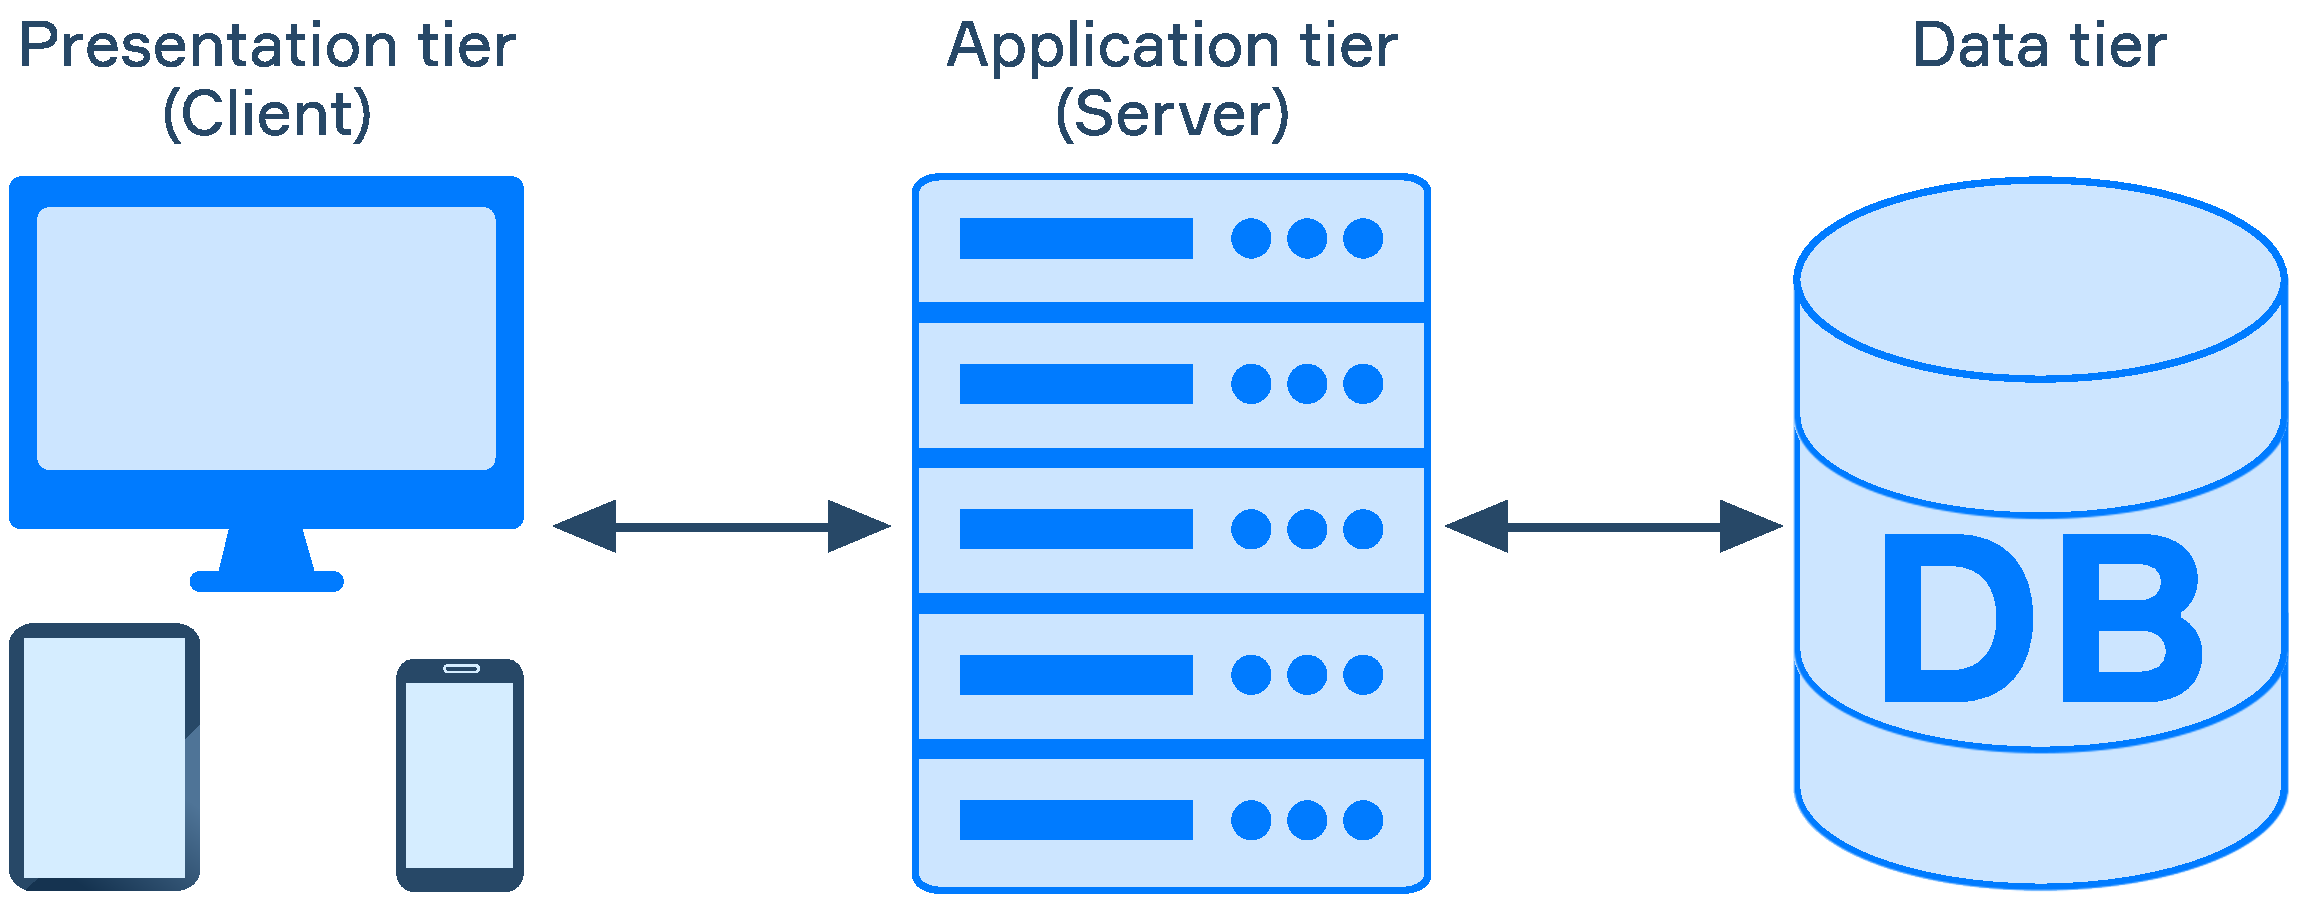
\includegraphics[width=0.7\columnwidth]{graphics/3-tier-arch.pdf}
	\caption{Three-tier Architecture \cite{3-tier}}
	\label{fig:3-tier}
\end{figure}


\begin{enumerate}
	\item \textbf{Presentation Layer (Client):}
	
	Handles all interactions with the user.
	Implements the user interface using ReactJS and Material UI.
	Communicates with the server through RESTful API calls and SocketIO for real-time features.
	Responsible for rendering components, collecting user input, and displaying data received from the backend.
	
	\item \textbf{Business Logic Layer (Server)}:
	
	NodeJS and ExpressJS handle the core business logic, such as processing support ticket requests, authenticating users, managing roles, and communicating with the database.
	SocketIO is used to manage real-time messaging between students and staff.
	Implements security features like JWT-based authentication and session management using Redis.
	
	\item \textbf{ Data Layer (Database)}:
	
	PostgreSQL stores all persistent data, including user profiles, support tickets, messages, and system logs.
	The server communicates with the database using SQL queries to retrieve, create, update, and delete records.
	Ensures data consistency and integrity by enforcing constraints, foreign keys, and relationships.
	
\end{enumerate}


\subsection{Frontend Design}












%	
	


	
\section{System Implementation}

\subsection{Frontend Implementation}

	\subsubsection{Source code structure}

\begin{longtable}{{|m{4.8cm}|m{9.6cm}|}} 
	\hline
	\textbf{Module/component name} & \textbf{Description}\\ \hline
	
	api/ & defines custom instance of api communication instance with the backend server.\\ \hline
	
	assets/ & contains all images and cascading style sheets.\\ \hline
	
	context/ & contains the constants which have to be shared across these components. \\ \hline
	
	hooks/ & contains custom React hooks. \\ \hline
	
	public/ & contains public assets (mostly for landing page). \\ \hline
	
	routes/ & defines all routes of the frontend. \\ \hline
	
	store/ & holds specific states of the frontend. \\ \hline
	
	themes/ & defines the color scheme, palette for the frontend. \\ \hline
	
	utils/ & contains shared utilities across components. \\ \hline
	
	views/ & contains main UI components for each roles. \\ \hline
	
	index.jsx & root component of the frontend. \\ \hline
	
	config.js & contains initial configuration of the front end. \\ \hline
	
	package.json & contains custom scripts and frontend package information. \\ \hline
	
	vite.config.mjs & contains configuration for Vite. \\ \hline
	
	\caption{Frontend source code structure} % needs to go inside longtable environment
	\label{tab:fe-src-code}
\end{longtable}

	\subsubsection{UI Main Components}
	\begin{figure}[H]
		\centering
		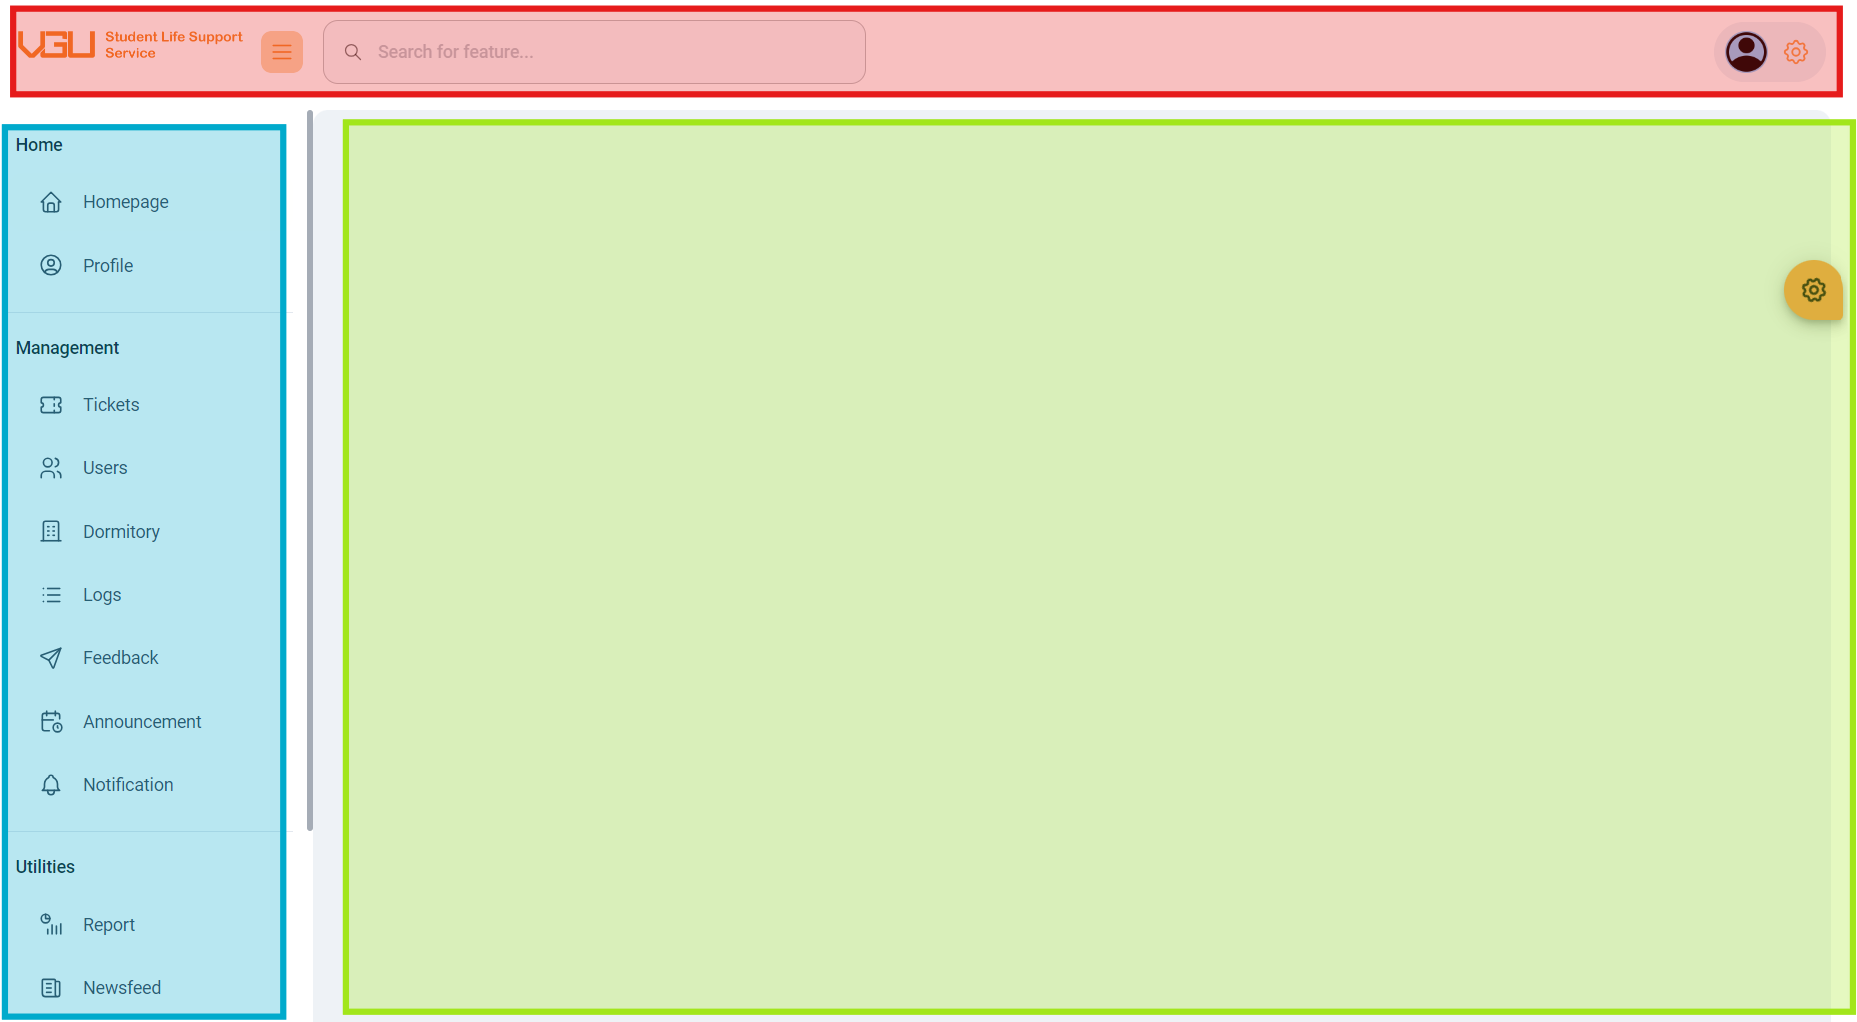
\includegraphics[width=1\linewidth]{graphics/fe/fe-main-comp}
		\caption{Web UI Main Components}
		\label{fig:fe-main-comp}
	\end{figure}
	There are 3 main components in the Web UI (marked on Figure \ref{fig:fe-main-comp}):
	
	\begin{enumerate}
		\item 	\colorbox{Salmon}{Header} (marked as Red color on Figure \ref{fig:fe-main-comp}) contains Logo image, Menu toggle button, Search bar, and Profile section  across all pages
		
\begin{lstlisting}[language=Javascript, breaklines=true, caption=Frontend Header Component]
const Header = ({ handleLeftDrawerToggle }) => {
	const theme = useTheme();
	
	return (
	<>
	{/* logo & toggler button */}
	<Box
	sx={{
			width: 228,
			display: 'flex',
			[theme.breakpoints.down('md')]: {
				width: 'auto'
			}
	}}
	>
	<Box component="span" sx={{ display: { xs: 'none', md: 'block' }, flexGrow: 1 }}>
	<LogoSection />
	</Box>
	<ButtonBase sx={{ borderRadius: '8px', overflow: 'hidden' }}>
	<Avatar
	variant="rounded"
	sx={{
			...theme.typography.commonAvatar,
			...theme.typography.mediumAvatar,
			transition: 'all .2s ease-in-out',
			background: theme.palette.secondary.light,
			color: theme.palette.secondary.dark,
			'&:hover': {
				background: theme.palette.secondary.dark,
				color: theme.palette.secondary.light
			}
	}}
	onClick={handleLeftDrawerToggle}
	color="inherit"
	>
	<IconMenu2 stroke={1.5} size="1.3rem" />
	</Avatar>
	</ButtonBase>
	</Box>
	
	{/* header search */}
	<SearchSection />
	<Box sx={{ flexGrow: 1 }} />
	<Box sx={{ flexGrow: 1 }} />
	

	{/* <ProfileSection /> */}
	<ProfileSection />
	</>
	);
};

Header.propTypes = {
	handleLeftDrawerToggle: PropTypes.func
};

export default Header;
\end{lstlisting}
		
		\item 	\colorbox{Aquamarine}{Sidebar} (marked as Blue color on Figure \ref{fig:fe-main-comp}): A dynamic navigation panel which renders all menu items of a specific roles.
		
\begin{lstlisting}[language=Javascript, breaklines=true, caption=Frontend Sidebar Component]
const Sidebar = ({ drawerOpen, drawerToggle, window }) => {
	const theme = useTheme();
	const matchUpMd = useMediaQuery(theme.breakpoints.up('md'));
	
	const drawer = (
	<>
	<Box sx={{ display: { xs: 'block', md: 'none' } }}>
	<Box sx={{ display: 'flex', p: 2, mx: 'auto' }}>
	<LogoSection />
	</Box>
	</Box>
	
	<BrowserView>
	<PerfectScrollbar
	component="div"
	style={{
			// height: !matchUpMd ? 'calc(100vh - 56px)' : 'calc(100vh - 88px)',
			height: !matchUpMd ? 'calc(100vh - 56px)' : 'calc(100vh - 88px)',
			paddingLeft: '16px',
			paddingRight: '16px'
	}}
	>
	<MenuList />
	{/* <MenuCard /> */}
	<Stack direction="row" justifyContent="center" sx={{ mb: 2 }}>
	<Chip label="v1.0.0" disabled chipcolor="secondary" size="small" sx={{ cursor: 'pointer' }} />
	</Stack>
	</PerfectScrollbar>
	</BrowserView>
	
	<MobileView>
	<Box sx={{ px: 2 }}>
	<MenuList />
	{/* <MenuCard /> */}
	<Stack direction="row" justifyContent="center" sx={{ mb: 2 }}>
	<Chip label="v1.0.0" disabled chipcolor="secondary" size="small" sx={{ cursor: 'pointer' }} />
	</Stack>
	</Box>
	</MobileView>
	
	</>
	);
\end{lstlisting}		
		
		
		
		
		
		\item  \colorbox{YellowGreen}{Content Components} (marked as Green color on Figure \ref{fig:fe-main-comp}): The content component will be displayed based on the matched predefined route. Once the route is determined, the content component is then lazy-loaded into the page. This means that the component will only be fetched and rendered when it is needed, which optimizes performance and improves loading times by minimizing the amount of initial content loaded.
		
		
\begin{lstlisting}[language=Javascript, breaklines=true, caption=Example of Lazy Loading Frontend Components]
const DashboardDefault = Loadable(lazy(() => import('views/homepage')));
const EditProfile = Loadable(lazy(() => import('views/EditProfile')));
const MyTickets = Loadable(lazy(() => import('views/MyTickets')));
\end{lstlisting}	
		
	\end{enumerate}
	
	
	\subsubsection{Responsive Design Implementation}
	Using Material-UI's grid system, responsive components, and utility features enables us to create a flexible and adaptive user interface in React applications. This ensures that the Web UI looks good and functions well on devices of all sizes, enhancing the overall user experience.
	
	\begin{enumerate}
		\item \textbf{Grid System}
		
		MUI provides a powerful Grid component that allows us to create responsive layouts easily. It uses a 12-column layout, and we can specify how many columns a component should span at different screen sizes.


\begin{lstlisting}[language=Javascript, breaklines=true, caption=MUI Grid System]
import { Grid } from '@mui/material';

	<Grid container spacing={2}>
		<Grid item xs={12} sm={6} md={4}>
			<Card>Content 1</Card>
		</Grid>
		
		<Grid item xs={12} sm={6} md={4}>
			<Card>Content 2</Card>
		</Grid>
	
		<Grid item xs={12} md={4}>
			<Card>Content 3</Card>
		</Grid>
	</Grid>
\end{lstlisting}		

	\item \textbf{Media Queries}
	
	MUI allows us to utilize CSS media queries through the sx prop or styles to create responsive designs that adapt to different screen sizes without much hassle.

\begin{lstlisting}[language=Javascript, breaklines=true, caption=MUI Media Queries]
<Box sx={{ 
		display: { xs: 'block', sm: 'flex' }, 
		flexDirection: { xs: 'column', sm: 'row' } 
}}>
{/* Our content */}
</Box>

\end{lstlisting}	


	\end{enumerate}
	
	
\newpage
\subsection{Backend Implementation}
	\subsubsection{Source code structure}
	
	\begin{longtable}{{|m{4.8cm}|m{9.6cm}|}} 
		\hline
		\textbf{Module/component name} & \textbf{Description}\\ \hline
		
		config/ & contains server configurations, database connection class, constants.\\ \hline
		
		controllers/ & contains API controllers.\\ \hline
		
		middleware/ & contains server middleware (token authentication, logger, mailer). \\ \hline
		
		routes/ & defines explicit API routes.  \\ \hline
		
		sql/ & contains all SQL queries. \\ \hline
		
		uploads/ & saves the user's uploaded attachments.\\ \hline
		
		utils/ & contains shared utilities across modules. \\ \hline
		
		index.js & root (start module) module of the backend server. \\ \hline
		
		package.json & contains custom scripts and backend packages information. \\ \hline
		
		.env & contains sensitive backend configurations. \\ \hline
		
		\caption{Backend source code structure} % needs to go inside longtable environment
		\label{tab:be-src-code}
	\end{longtable}
	
	
	\subsubsection{Setting up ExpressJs Server}
	The implementation below sets up a web server with essential middleware and route handling for a robust application. It initializes the app, enabling JSON parsing, cookie parsing, and Cross-Origin Resource Sharing (CORS) with restricted options. The server then defines various API endpoints for authentication and resource management, including user, dorm, ticket, attachment, rating, message, role, notification, announcement, feedback, logs, and reports. Each route corresponds to a specific functionality, organized under the /auth and /api/v1/ prefixes, ensuring a structured and scalable approach to managing the application’s various services.

\begin{lstlisting}[language=Javascript, breaklines=true, caption=ExpressJS Server Setup]
const app = express();
app.use(express.json());
app.use(cookieParser()); // Enable cookie parsing
app.use(cors(WebConfig.corsOptions));


// ==============================|| Routes ||============================== //
app.use("/auth", authRoutes);                     
app.use("/api/v1/users", userRoutes);                  
app.use("/api/v1/dorms", dormRoutes)
app.use("/api/v1/tickets", ticketRoutes);        
app.use("/api/v1/attachments", attachmentRoutes); 
app.use("/api/v1/rating", ratingRoutes);          
app.use("/api/v1/messages", messageRoutes);
app.use("/api/v1/roles", roleRoutes);       
app.use("/api/v1/notification", notificationRoutes); 
app.use("/api/v1/announcement", announcementRoutes);        
app.use("/api/v1/feedback", feedbackRoutes);       
app.use("/api/v1/logs", logsRoutes);     
app.use("/api/v1/reports", reportRoutes);
\end{lstlisting}	

	\subsubsection{Database Integration}
	
\begin{lstlisting}[language=Javascript, breaklines=true, caption=Server connects to PostgreSQL Database]
import pkg from 'pg';
import dotenv from 'dotenv';

dotenv.config();

const { Pool } = pkg;

const pool = new Pool({
	user: String(process.env.PG_DB_USER),
	host: String(process.env.PG_DB_HOST),
	password: String(process.env.PG_DB_PASSWORD),
	port: Number(process.env.PG_DB_PORT),
	database: String(process.env.PG_DB_DATABASE),
});

export default pool;  
\end{lstlisting}	


\begin{lstlisting}[language=Javascript, breaklines=true, caption=Server connects to Redis]
import redis from 'redis';

const redisClient = redis.createClient({
	socket: {
		host: process.env.REDIS_HOST,
		port: process.env.REDIS_PORT,
	},
});


const connectRedis = async () => {
	await redisClient.connect();
	redisClient.on('error', (err) => {
		console.error('Redis error:', err);
	});
	console.log('Redis connected successfully');
};
\end{lstlisting}	


\subsubsection{Middleware}
In the system, the \texttt{authenticateToken} middleware is designed to protect API endpoints by verifying JWT (JSON Web Tokens) based on user roles. The authenticateToken function accepts an array of allowedRoles, which specifies which user roles are permitted to access the route that this middleware protects. The middleware checks for a valid access token in the request headers and verifies it against predefined secrets corresponding to different user roles (e.g., student, staff, admin).

Additionally, \texttt{logger} - an asynchronous middleware designed to log events to a PostgreSQL database. This function serves as a logging mechanism, capturing important user actions or system events and storing them in a dedicated "Log" table. 
\begin{lstlisting}[language=Javascript, breaklines=true, caption= Logger middleware - write log to database]
const writeLogToDB = async (user_id, event_id, description, timestamp) => {
	try {
		await pool.query('BEGIN');
		await pool.query(
		'INSERT INTO "Log" (user_id, event_id, description, timestamp) VALUES ($1, $2, $3, $4)',
		[user_id, event_id, description, timestamp]
		);
		await pool.query('COMMIT');
		logger.info('Log written to database');
	} catch (error) {
		await pool.query('ROLLBACK');
		logger.error(error);
	}
};
\end{lstlisting}	

\subsubsection{Real-time messages}
By creating an HTTP server that integrates with the existing Express application. The Socket.IO server is attached to this HTTP server, allowing for real-time communication over web sockets.

\begin{lstlisting}[language=Javascript, breaklines=true, caption=Create Socket.io HTTP server]
const server = http.createServer(app);
const io = new Server(server, {
	cors: {
		origin: WebConfig.corsOptions.origin,
		methods: ['GET', 'POST'],
	},
});
\end{lstlisting}	



The backend sets up an event listener for incoming connections using the \texttt{io.on('connection')} method. This function is triggered whenever a new user connects to the server. When a user joins a conversation, they emit a \texttt{join\_conversation} event along with the \texttt{ticket\_id} of the conversation.

\begin{lstlisting}[language=Javascript, breaklines=true, caption=Socket.io join\_conversation event]
socket.on('join_conversation', (ticket_id) => {
	socket.join(ticket_id);
	console.log(`User joined conversation ${ticket_id}`);
});
\end{lstlisting}	

When a user sends a message, they emit a \texttt{send\_message} event with the message details. This event is processed to store the message in the database and then broadcast it to other users in the same conversation.


\begin{lstlisting}[language=Javascript, breaklines=true, caption=Socket.io send\_message event]
socket.on('send_message', async (data) => {
	const { ticket_id, sender_id, message_details } = data;
	const created_date = new Date();
	
	try {
		await pool.query('BEGIN'); // Start a transaction
		
		// Insert messages data into database
		
		await pool.query('COMMIT'); // Commit the transaction
		
		io.to(ticket_id).emit('receive_message', newMessage); // Emit the new message to the room
	} catch (err) {
		await pool.query('ROLLBACK'); // Rollback in case of error
		console.error(err);
	}
});

\end{lstlisting}	

Lastly, the disconnect event is implemented to clean up and log when a user disconnects from the conversation.
\begin{lstlisting}[language=Javascript, breaklines=true, caption=Socket.io disconnect event]
socket.on('disconnect', () => {
	console.log('A user disconnected from the conversation');
	// Handle clean up
});
\end{lstlisting}

\newpage
\subsection{Security Measures}
	\subsubsection{JWT Authentication/Authorization}
	\begin{figure}[H]
		\centering
		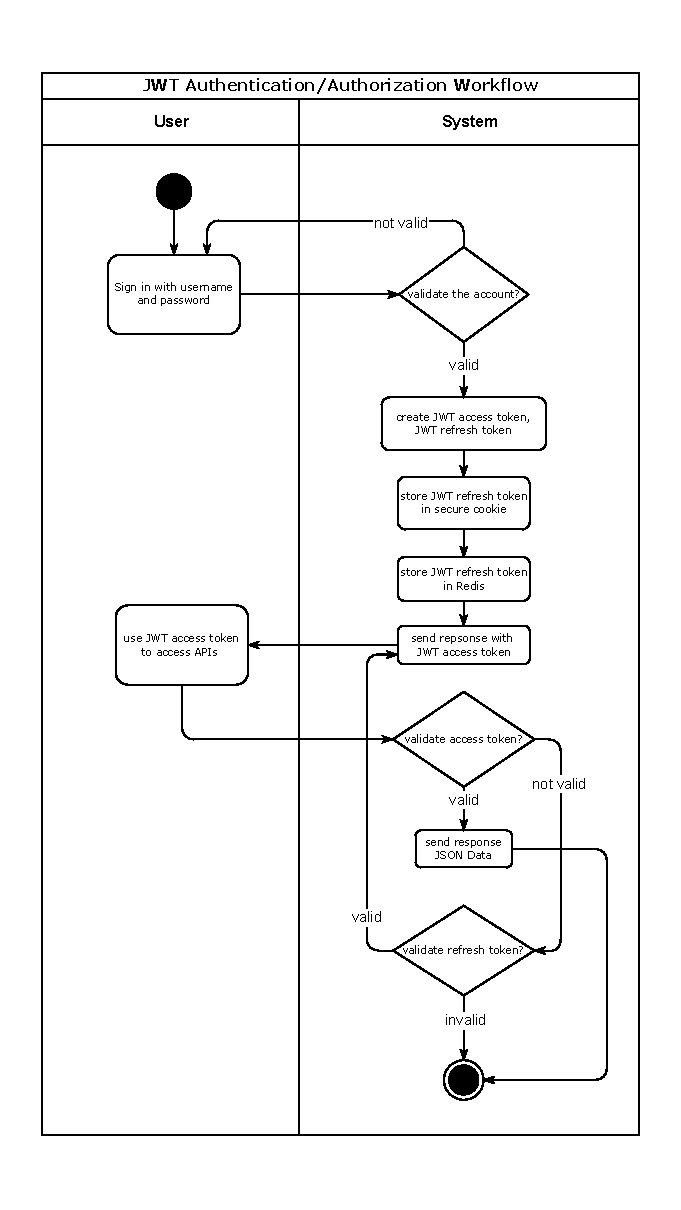
\includegraphics[width=0.58\columnwidth]{graphics/jwt-auth.pdf}
		\caption{JWT Authentication/Authorization Workflow}
		\label{fig:jwt-auth}
	\end{figure}
	
	The JWT (JSON Web Token) authentication and authorization workflow in the Student Life Support Service is designed to ensure secure access to the system's resources while providing a seamless user experience. The process begins when a user signs in by submitting their credentials, such as a username and password. Upon successful validation of these credentials, the system generates two tokens: an access token and a refresh token. The access token is used for short-term authorization and is typically included in the Authorization header of API requests to grant the user access to protected resources. 
	
	\noindent To ensure a high level of security, the refresh token is stored in two secure locations: a cookie on the client-side and in Redis, which serves as an in-memory database for managing sessions. The refresh token allows the system to issue a new access token when the original one expires, ensuring that the user does not need to log in repeatedly.
	
	\noindent When a user makes an API request, the system first checks the validity of the provided access token. If the token is valid, the request is processed, and the appropriate data is returned. However, if the access token is expired or invalid, the system turns to the refresh token. If the refresh token is verified as valid, a new access token is generated, and the user can continue to access the API without re-authenticating.
	
	\noindent In cases where both the access and refresh tokens are invalid, the user is required to log in again, ensuring that expired or tampered tokens do not grant unauthorized access to the system. By utilizing this access-refresh token structure, with refresh tokens stored securely in Redis and cookies, the system balances both security and usability, providing users with continuous access while protecting against unauthorized usage or token expiration.
	
	\noindent This approach ensures that the system is scalable and can handle multiple user sessions efficiently, while also offering robust security through token validation and management.

\begin{lstlisting}[language=Javascript, breaklines=true, caption=Store refresh token in secure cookie]
// Send Refresh Token as an HTTP-only, Secure cookie
res.cookie('refreshToken', refreshToken, {
	httpOnly: true,       					// Prevent JavaScript access to the cookie
	secure: true,         					// Send only over HTTPS
	sameSite: 'Strict',   					// Protect against CSRF
	maxAge: REFRESH_TOKEN_EXPIRED_IN * 1000, 
});
\end{lstlisting}

	\subsubsection{Password Hashing}
	All user passwords within the system are securely protected through the use of a one-way hashing algorithm. This is accomplished by employing the \texttt{\textbf{bcryptjs}} library, which ensures that passwords are irreversibly encrypted, thereby enhancing the security and integrity of user credentials. \\
	
	The \texttt{\textbf{hashPassword}} function below takes a user's plaintext password as input and securely hashes it. First, the function generates a salt using bcrypt.genSalt, which adds an extra layer of randomness to the hashing process. This salt is combined with the user's password using the bcrypt.hash function to create a unique hashed version of the password. The hashed password is then returned, ensuring that even if the same password is used by multiple users, the stored hash will be different due to the unique salt for each password. In case of any errors during this process, the function throws a detailed error message for debugging purposes.
	
\begin{lstlisting}[language=Javascript, breaklines=true, caption=Password Hashing]
async function hashPassword(userInputPassword) {
	try {
		const salt = await bcrypt.genSalt(saltRounds);
		const hash = await bcrypt.hash(userInputPassword, salt);
		return hash; // Return the hashed password
	} catch (error) {
		throw new Error('Error hashing password: ' + error.message);
	}
}
\end{lstlisting}

	The verifyPassword function is used to check if a user's inputted password matches the stored hashed password in the system. It does this by using bcrypt.compare, which compares the plaintext password with the hashed password stored in the database. If the passwords match, the function returns true; otherwise, it returns false. Similar to hashPassword, if an error occurs during the verification process, an error message is thrown for further investigation.
	
\begin{lstlisting}[language=Javascript, breaklines=true, caption=Password Verification]
async function verifyPassword(userInputPassword, encryptedPassword) {
	try {
		const isMatch = await bcrypt.compare(userInputPassword, encryptedPassword);
		return isMatch;
	} catch (error) {
		throw new Error('Error verifying password: ' + error.message);
	}
}
\end{lstlisting}
	
	
	
	\subsubsection{Google reCAPTCHA}
	Google reCAPTCHA is a security service designed to protect websites from bots and automated abuse. It uses a combination of behavioral analysis, machine learning, and user challenges to distinguish between human users and malicious bots. The main goal of reCAPTCHA is to prevent attacks such as credential stuffing, brute-force attempts, and other forms of automated exploits while allowing legitimate users to interact with the site without interruption. \cite{google-recaptcha}
	
	In this system, integrating reCAPTCHA in the "Edit Profile" and "Change Password" features enhances security by preventing automated attacks and brute-force attempts. It ensures that only legitimate users can make critical changes, reducing the risk of unauthorized access and data breaches. reCAPTCHA also helps protect sensitive user information, adds an extra layer of verification for critical actions, and prevents abuse or spam, maintaining system integrity and keeping accounts secure.
	\begin{figure}[H]
		\centering
		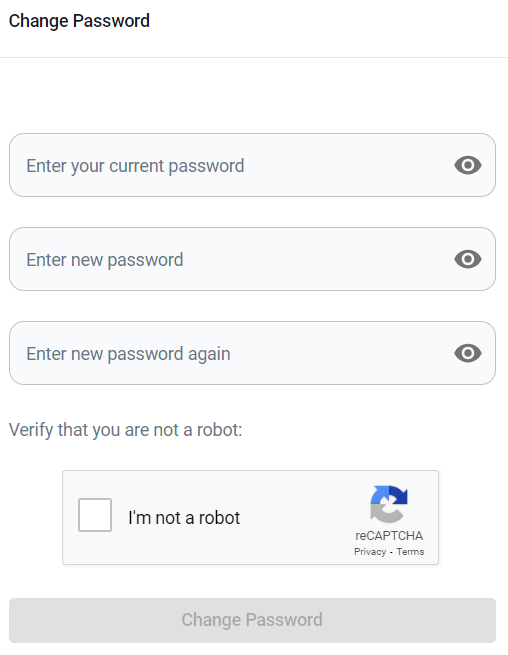
\includegraphics[width=0.3\linewidth]{graphics/change-password-captcha}
		\caption{reCAPTCHA in Change Password form}
		\label{fig:change-password-captcha}
	\end{figure}
	
	
	
	
	
	
\section{User Manual}

\subsection{Sign in}
\begin{figure}[H]
	\centering
	
\includegraphics[width=1.\linewidth]{graphics/gui/user/landing}
	\caption{Landing page}
	\label{fig:landing}
\end{figure}

In the landing page of the service, navigate to Login page by clicking "Sign In Now"


\begin{figure}[H]
	\centering
	\begin{minipage}{.5\textwidth}
		\centering
		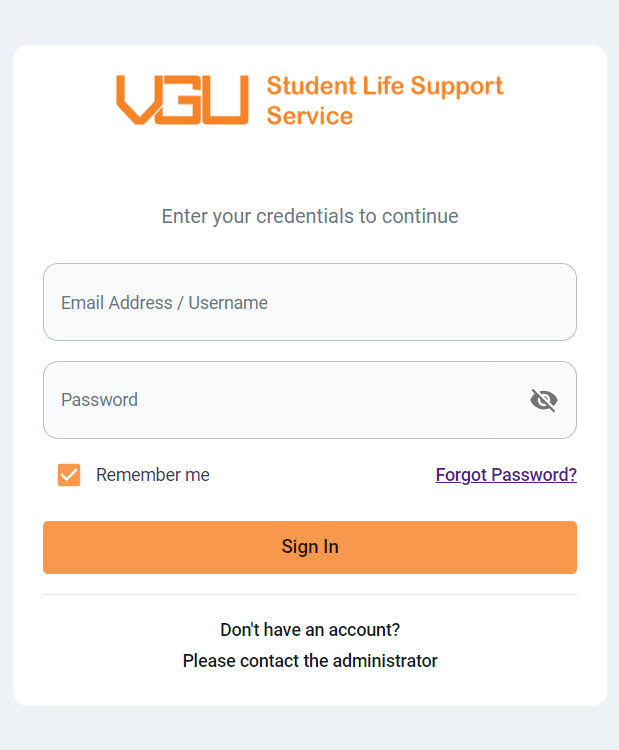
\includegraphics[width=.9\linewidth]{graphics/gui/user/login.png}
		\captionof{figure}{Sign in Form}
		\label{fig:gui-login}
	\end{minipage}%
	\begin{minipage}{.5\textwidth}
		\centering
		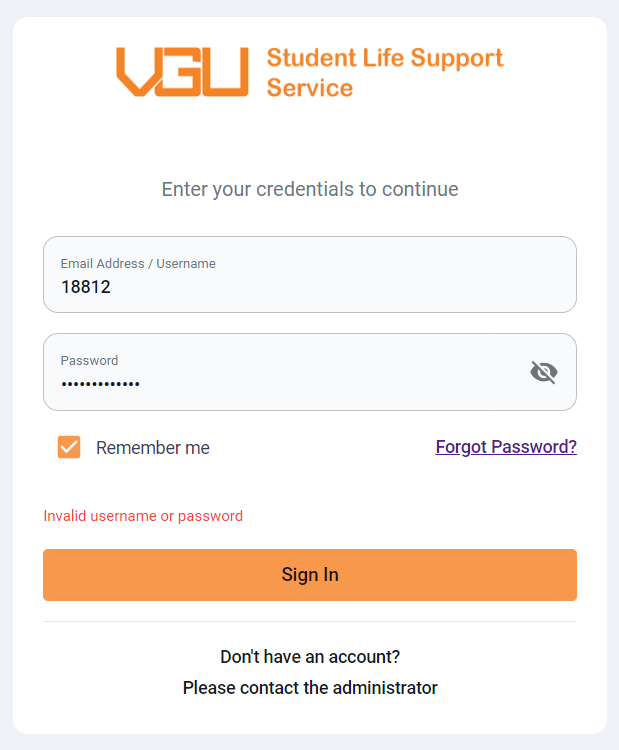
\includegraphics[width=0.9\linewidth]{graphics/gui/user/login-error.png}
		\captionof{figure}{Failed Sign in attempt}
		\label{fig:gui-login-failed}
	\end{minipage}
\end{figure}



To access the service, input your username (or email) and password, then click on the sign-in button (refer to Figure \ref{fig:gui-login}). If you provide incorrect credentials, a warning message will appear, indicating that you need to correct either your username or password (Figure \ref{fig:gui-login-failed}).





\subsection{Forgot password}

%In case of forgetting your password, you can reset it by clicking 'Forgot Password?' of the 'Sign in' form (see Firgure \ref{fig:gui-login}). Then, enter your the email in the 'Forgot Password' form adn click 'Reset Password' (Figure \ref{fig:gui-forgot-pass})

If you forget your password, you can initiate a reset by selecting the 'Forgot Password?' option on the 'Sign in' form (refer to Figure \ref{fig:gui-login}). Subsequently, provide your email address in the 'Forgot Password' form and click on 'Reset Password' (see Figure \ref{fig:gui-forgot-pass}).

\begin{figure}[H]
	\centering
	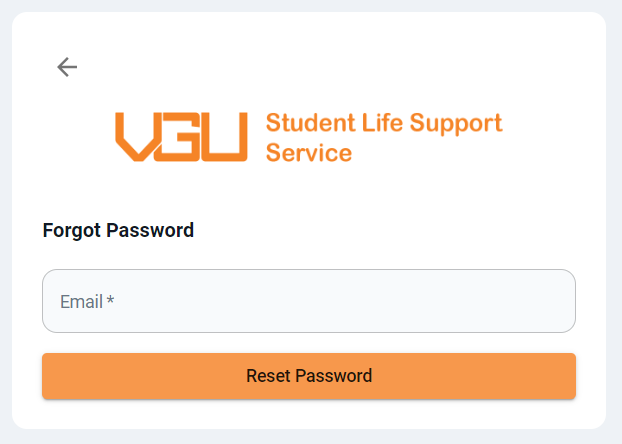
\includegraphics[width=0.7\linewidth]{graphics/gui/user/reset-pass.png}
	\caption{Reset password form}
	\label{fig:gui-forgot-pass}
\end{figure}



If your email is associated with an account in the system, a success notification will appear, and password reset instructions will be sent to your email (Figure \ref{fig:gui-reset-pass-success}, \ref{fig:gui-email-reset-pass}).  Conversely, if the email is not found in the system, a failure notification will indicate that the email does not exist (Figure \ref{fig:gui-reset-pass-failed}).

\begin{figure}[H]
	\centering
	\begin{minipage}{.5\textwidth}
		\centering
		
\includegraphics[width=.9\linewidth]{graphics/gui/user/reset-pass-success.png}
		\captionof{figure}{Reset password successfully}
		\label{fig:gui-reset-pass-success}
	\end{minipage}%
	\begin{minipage}{.5\textwidth}
		\centering
		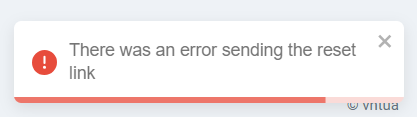
\includegraphics[width=0.9\linewidth]{graphics/gui/user/reset-pass-failed.png}
		\captionof{figure}{Reset password failed}
		\label{fig:gui-reset-pass-failed}
	\end{minipage}
\end{figure}


\begin{figure}[H]
	\centering
	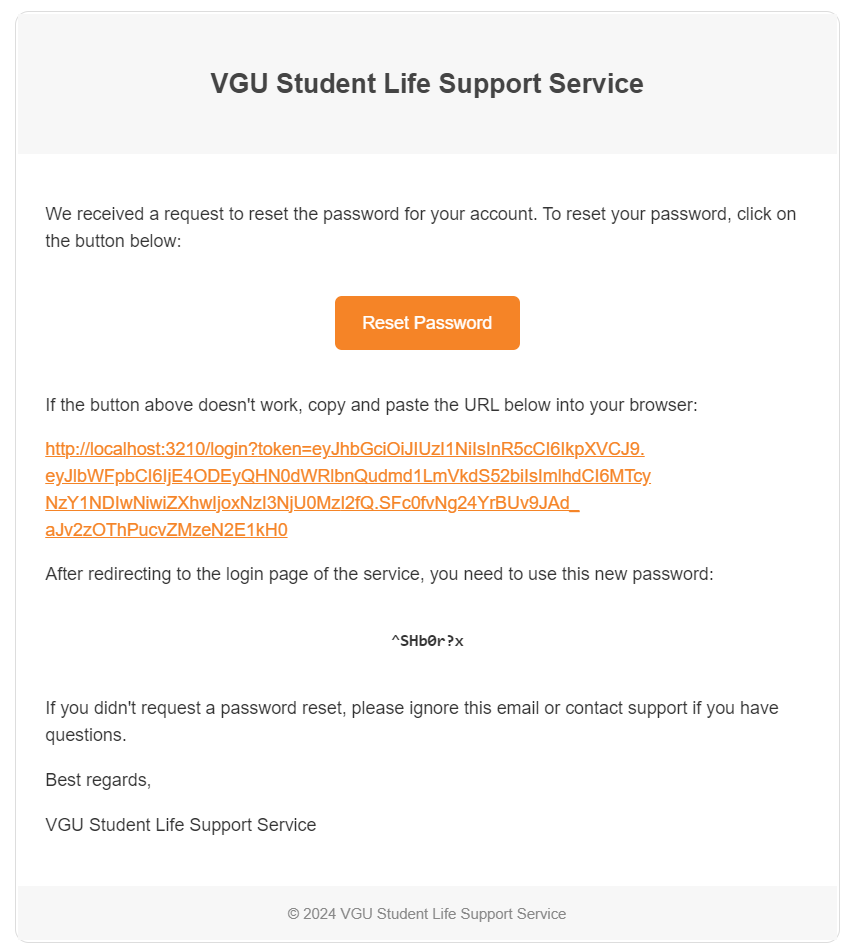
\includegraphics[width=0.8\linewidth]{graphics/gui/user/email-reset.png}
	\caption{Reset password email instructions}
	\label{fig:gui-email-reset-pass}
\end{figure}





\section{Conclusion and Future Work}


\subsection{Conclusion}

In conclusion, the Student Life Support Service web application represents a significant advancement in the way students can access and manage essential resources. By leveraging modern technologies such as ReactJS, Material UI, NodeJS, and PostgreSQL, the application provides a robust and responsive platform that meets the dynamic needs of its users. The use of ReactJS enables the creation of a seamless user interface, fostering an intuitive navigation experience. Material UI enhances this by offering a comprehensive set of pre-designed components that streamline the development process and maintain a consistent aesthetic across the application. \\ \\
The backend, built with NodeJS and ExpressJS, ensures efficient data handling and real-time interactions through the implementation of SocketIO. This combination allows for swift processing of requests and timely updates, critical for a platform designed to support communication among students and staff. PostgreSQL's strong ACID compliance guarantees the integrity and reliability of data, which is crucial for managing sensitive information such as user accounts and communication logs. \\ \\
Throughout the development process, extensive attention has been paid to user experience. The application is designed to be responsive, catering to various devices and screen sizes, which is essential in today’s mobile-first world. Furthermore, thorough testing and validation have been conducted to ensure the application functions smoothly, providing users with a dependable resource for support and information. \\ \\
Looking ahead, the project has laid a strong foundation for future enhancements. As the needs of students evolve and grow, so too must the capabilities of the application. By focusing on areas such as dynamic role management, scalability, and improved handling of concurrent user requests, the Student Life Support Service can adapt to changing user demands while ensuring high performance and security. \\ \\
In essence, the development of this web application is not merely an endpoint but the beginning of an ongoing journey. The commitment to continuous improvement will ensure that the platform remains relevant and valuable to students, supporting their academic and social endeavors in an increasingly digital world. With a clear vision for future enhancements and a solid technical foundation, the Student Life Support Service is poised to significantly impact student life on campus, promoting engagement and accessibility like never before.

\subsection{Future Work}
There are several key areas for improvement and expansion have been identified in the future:

	\begin{enumerate}
		\item \textbf{Dynamic Role Management:} Implementing a dynamic role management system will enhance the application’s flexibility. This feature will allow administrators to create and assign specific permissions to different user roles, tailoring access and functionality based on user needs. By enabling fine-grained control over resource access, the system can better accommodate various user requirements and enhance security.
		
		\item \textbf{Scalability:} To ensure the application can handle a growing number of users and increased data load, scalability must be a primary focus. This involves optimizing the architecture to support horizontal scaling, which can be achieved by implementing load balancers and distributing requests across multiple server instances. Additionally, strategies such as microservices architecture can be explored to further enhance scalability and maintainability.
		
%		\item \textbf{Handling High Concurrent User Requests:} Improving the application’s ability to handle high volumes of simultaneous user requests is crucial for maintaining performance and user satisfaction. Techniques such as caching strategies (using Redis or similar technologies) can significantly reduce database load and improve response times. Additionally, optimizing database queries and utilizing connection pooling can further enhance the system's efficiency under heavy load.
	\end{enumerate}
	
\noindent By addressing these future work areas, the Student Life Support Service web application can continue to evolve and better serve its users in reality, ensuring a reliable and efficient platform for student engagement and support.





% ========================================= SAMPLE ===================================

%\section{Tuna Code Sample}

% Example R code block
\begin{lstlisting}[language=R, caption=Example R Code to Calculate Distance]
	# Calculate the points distance
	point_dist <- dist(df_dummy, method = "canberra")      # Using Canberra distance
\end{lstlisting}


\begin{lstlisting}[language=Javascript, caption=Example JS Code]
	function addNumbers(a, b) {
		if (typeof a !== 'number' || typeof b !== 'number') {
			console.error('Both arguments must be numbers');
			return null;
		}
		const sum = a + b;
		return sum;
	}
	// Handle const
	
	async function fetchData(url) {
		try {
			const response = await fetch(url);
			const data = await response.json();
			return data;
		} catch (error) {
			console.error('Error fetching data:', error);
		}
	}
	
	console.log(addNumbers(5, 10));
	fetchData('https://api.example.com/data');
\end{lstlisting}
%\section{Tuna Image Imports}

\includesvg[width=0.4\columnwidth]{chapters/example/Untitled Diagram-Page-1.drawio.svg}

% Use inkscape for exporting the .svg image to pdf, then import the image
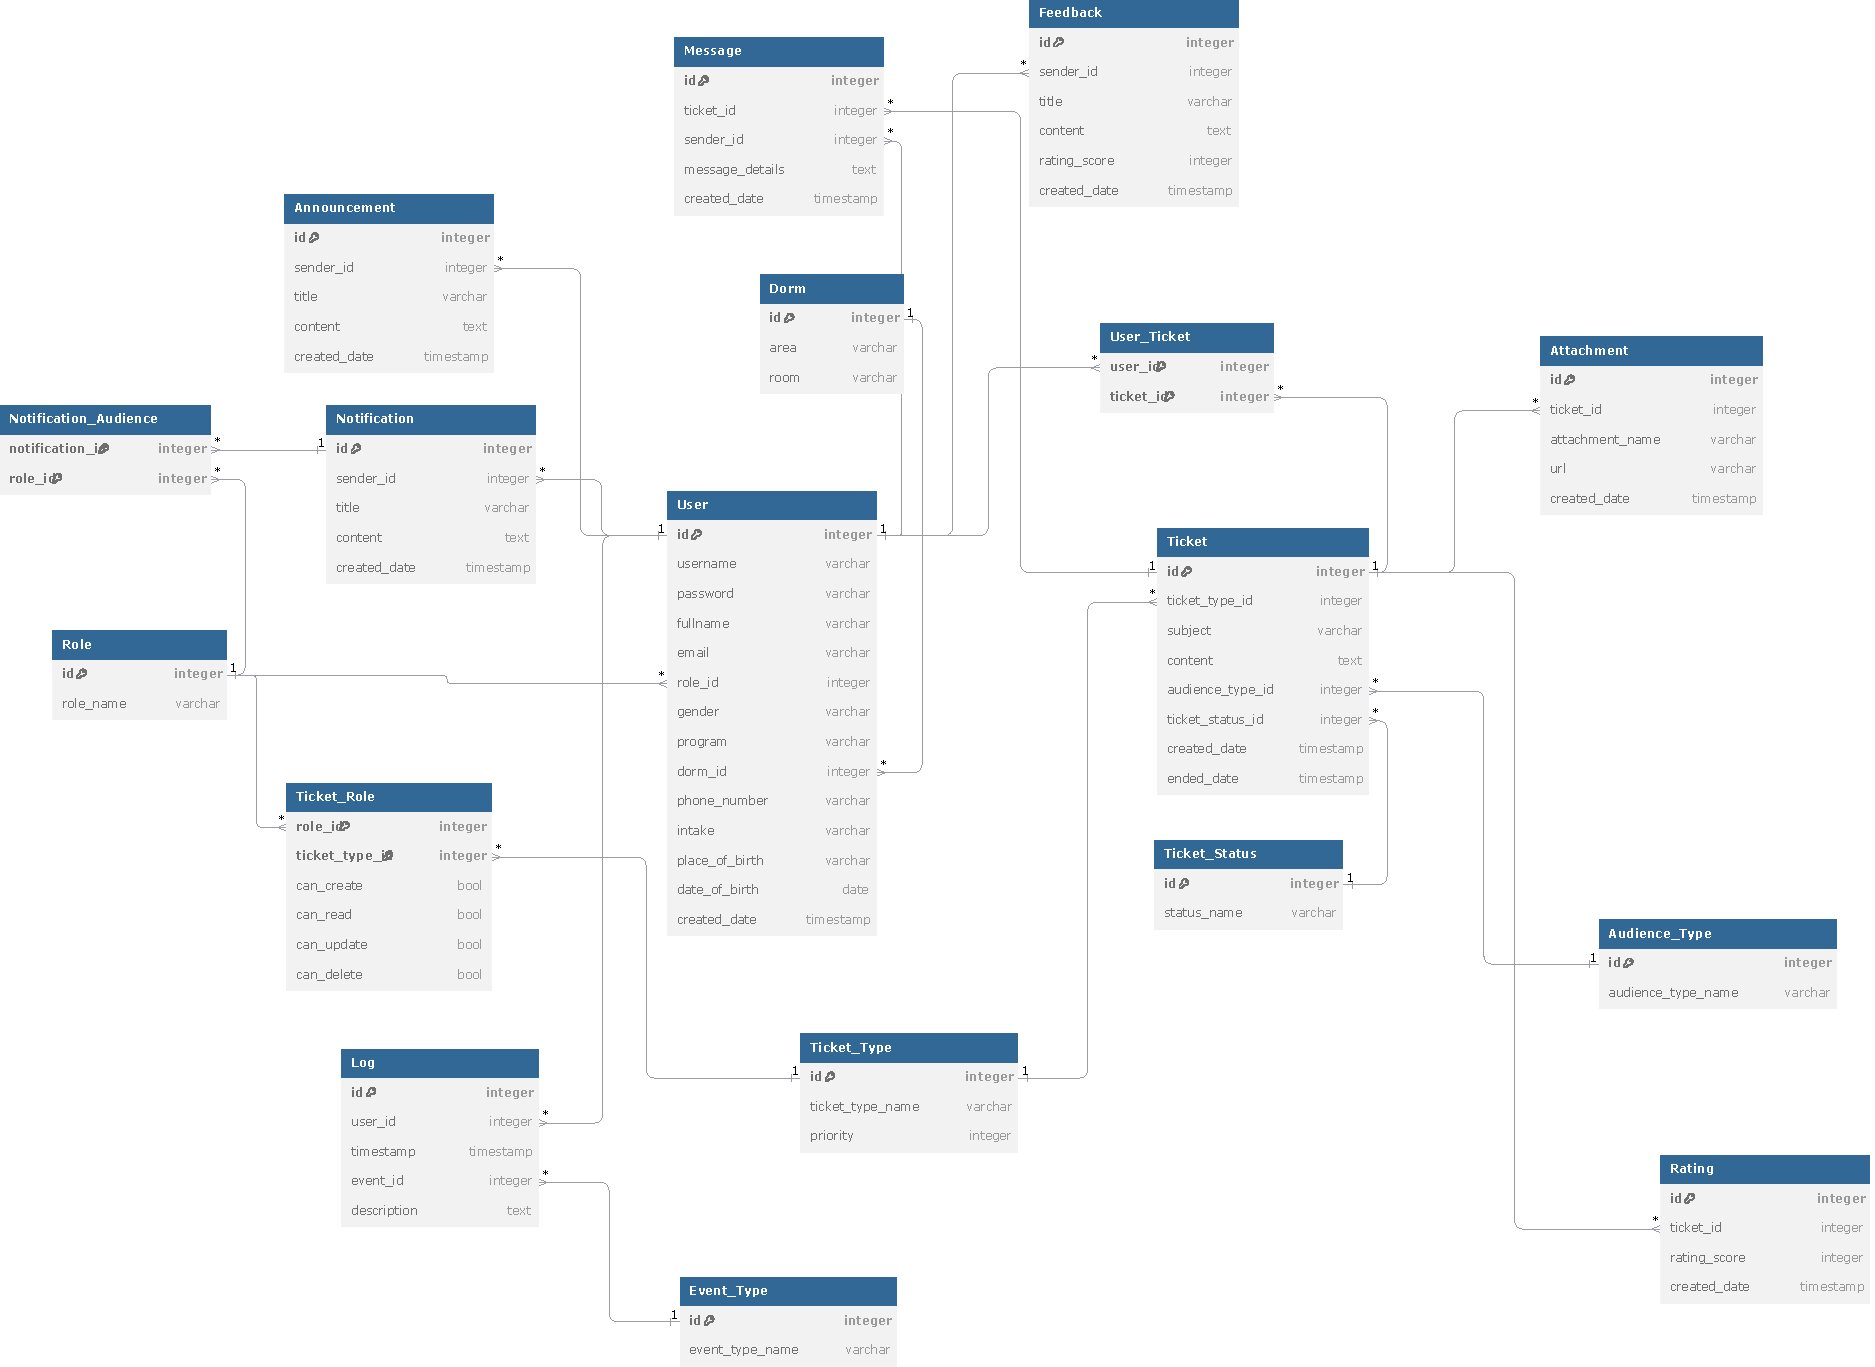
\includegraphics[width=0.4\columnwidth]{chapters/example/db-drawio.pdf}

%\acuseall



%\ac{usa}, \ac{usa}
%
%\ac{eu}, \ac{eu}
%
%\ac{ussr}, \ac{ussr}


% \newpage




%\section{Company Overview}

\subsection{Origin and Inception}
% Bosch Global Software Technologies Vietnam (BGSW Vietnam) was established as part of the Bosch Group's strategic expansion into Southeast Asia, aimed at leveraging the region's growing technological capabilities and dynamic talent pool. Incepted in 2010, BGSW Vietnam began as a development center designed to support Bosch's global operations with high-quality software solutions. Situated in Ho Chi Minh City, a burgeoning tech hub, the center was positioned to tap into Vietnam's skilled workforce and rapidly developing IT infrastructure. The inception of BGSW Vietnam was driven by Bosch's recognition of Vietnam's potential to contribute significantly to its global innovation ecosystem. Over the years, BGSW Vietnam has expanded its scope, providing comprehensive services in software development, IT consulting, and digital transformation to various sectors, including automotive, manufacturing, and consumer electronics. This expansion underscores Bosch's commitment to integrating advanced software engineering with traditional manufacturing excellence, fostering innovation and enhancing operational efficiencies. BGSW Vietnam's growth trajectory reflects Bosch's broader strategy of establishing a robust global network of innovation centers, dedicated to delivering cutting-edge technological solutions and maintaining competitive advantage in an increasingly digital world.

Bosch Global Software Vietnam (BGSW Vietnam) was established in 2010 as a wholly-owned subsidiary of the Robert Bosch GmbH, the multinational engineering and technology company headquartered in Gerlingen, Germany. BGSW Vietnam was founded in Ho Chi Minh City, Vietnam as part of Bosch's strategic initiative to expand its global software development capabilities and leverage Vietnam's growing talent pool of skilled software engineers.\cite{company_overview_about_us} \\ \\
The decision to set up a software development center in Vietnam was driven by several factors. Vietnam's rapidly developing information technology (IT) industry, coupled with a large and well-educated workforce, presented an attractive opportunity for Bosch to tap into a new source of software engineering talent. Additionally, Vietnam's favorable economic climate, including competitive labor costs and government incentives for foreign investment in the tech sector, made it a compelling location for Bosch to establish its latest software R\&D facility. \\ \\
In its early years, BGSW Vietnam's primary focus was on developing software solutions for the automotive industry, including embedded systems, connectivity features, and cloud-based services for Bosch's range of automotive products. Over time, the company has expanded its scope to encompass a broader range of software domains, contributing to various Bosch products and services across different business sectors, such as industrial technology, consumer goods, and energy and building technology. \\ \\
Today, BGSW Vietnam plays a key role in Bosch's global R\&D footprint, serving as a center of excellence for software innovation. The company has continuously grown its workforce of Vietnamese software professionals, leveraging the country's strong technical education system and vibrant IT ecosystem to support Bosch's global software development initiatives.

% 90\% of employees at Bosch Global Software Technologies Vietnam say it is a great place to work compared to 53\% of employees at a typical Global company

\subsection{Main products}
Bosch Global Software Technologies Vietnam (BGSW Vietnam) is renowned for delivering a wide array of advanced software solutions and services tailored to meet the diverse needs of various industries. Among its primary offerings, BGSW Vietnam excels in developing embedded software for the automotive industry, including advanced driver assistance systems (ADAS), powertrain control, and infotainment systems. These solutions are pivotal in enhancing vehicle safety, efficiency, and user experience. Additionally, BGSW Vietnam provides robust IT services encompassing application development, system integration, and IT infrastructure management, which are crucial for digital transformation initiatives across multiple sectors. The company also specializes in IoT solutions, harnessing the power of connected devices to drive innovation in smart manufacturing, home automation, and industrial automation. Furthermore, BGSW Vietnam offers cutting-edge AI and machine learning solutions, enabling businesses to leverage data analytics for informed decision-making and improved operational efficiencies. This comprehensive suite of products and services positions BGSW Vietnam as a key player in the global software technology landscape, contributing significantly to Bosch’s mission of creating intelligent and sustainable solutions for a connected world.
%\section{Internship Description}

\subsection{Internship experience overview}

    \subsubsection{Workplace}
    The office in which I was employed is situated in the Etown Building, located at 364 Cong Hoa Street, Ward 13, Tan Binh District, Ho Chi Minh City, Vietnam. The building is well-appointed with modern amenities, including a high-quality lighting system conducive to visual comfort, ergonomic chairs, solid desks, and high-speed internet access. My designated workspace was in the "Talent pool" area of the floor, where all interns were assigned. For professional purposes, I was provided with a high-specification desktop computer to facilitate my work.

        
    \subsubsection{Language and formal communication}
    Within the professional environment, I employed both English and Vietnamese for interpersonal communication. Given that the majority of my colleagues were Vietnamese, I primarily used Vietnamese for information sharing. However, in regard to the reporting procedures and written documents, it was explicitly mandated that the reports be composed in the English language.
    
    \subsubsection{The project team}
    Our team comprises three members, each assigned specific roles that contribute to the project's success. We follow the Agile software development methodology, which defines roles such as Product Owners, Team Lead, and Development Team. Given the limited team size, I assume dual responsibilities, functioning both as the Team Lead and as a member of the Development Team (Backend developer).

    \subsubsection{Project specification and process}
    
    The internal project's objective is to build a web application which helps managers monitor the monthly efforts of each employee, plan and report the billing information list. This involves a comprehensive understanding of the requirements, the billing data and the structure of all components. It requires us to analyse the requirements and application backlog carefully and collaborate closely with the Product Owner as well as the Customer.

    To effectively fulfill these responsibilities, we adhere to the Agile software development methodology, as previously outlined. Our team employs a standardized approach that centers on three primary domains: analysis, implementation, and reporting. Each sprint is scheduled on a weekly basis, with the team dedicating their efforts to achieving the sprint goal until its conclusion. Upon completion of the sprint, we conduct a two-hour meeting during which we discuss task progress, completed work, encountered challenges, and plans for the subsequent sprint.
    
    \subsubsection{Team communication}

    \begin{tabular}{ @{} m{0.25\textwidth} m{0.7\textwidth} @{} }
      \begin{minipage}{\linewidth}
        \centering
        
\includegraphics[width=0.7\linewidth]{graphics/ms-teams-logo.jpg}
        \captionof{figure}{Microsoft Teams platform}
        \label{fig:ms-teams-logo}
      \end{minipage}
      &
      \begin{minipage}{\linewidth}
            For communication with each other in a team, we use Microsoft Teams platform.  Moreover, it is imperative that employees are assigned to specific channels within Slack that align with their respective tasks and responsibilities in the workplace. This ensures a streamlined and efficient flow of information, facilitates task-related discussions and collaborations, and contributes to the overall effectiveness and productivity within the organizational framework.
      \end{minipage}
    \end{tabular}

    
    \subsubsection{Task assignment}
 %    \begin{figure}[H]
	% 		\centering
	% 		
\includegraphics[scale=0.2]{graphics/openproject-logo.png}
	% 		\caption{OpenProject project management platform}
	% 		\label{fig:openProject}
	% \end{figure}
    \begin{figure}[H]
        \centering
        \begin{minipage}{.5\textwidth}
          \centering
          
\includegraphics[width=.4\linewidth]{graphics/ms-project.png}
          \captionof{figure}{Microsoft Project}
          \label{fig:msProject}
        \end{minipage}%
        \begin{minipage}{.5\textwidth}
          \centering
          
\includegraphics[width=.4\linewidth]{graphics/openproject-logo.png}
          \captionof{figure}{OpenProject}
          \label{fig:openProject}
        \end{minipage}
    \end{figure}

    In the training phase, I was assigned tasks on the Microsoft Project board by my manager. I had to follow the schedule to complete the training tasks. The structure of the task board based on the waterfall project management framework, means that I have to complete the previous task to do the next one. The schedule, in general is well-defined, and I can follow the timeline smoothly. \\
    
    The reason why Microsoft Project platform is used is that it is a robust project management software developed by Microsoft, widely utilized across various industries for its comprehensive tools that facilitate project planning, scheduling, resource allocation, and progress tracking. One of its primary advantages is its ability to manage complex projects with multiple interconnected tasks through Gantt charts, which provide a visual timeline of project activities and dependencies. This feature allows project managers to effectively schedule tasks, allocate resources, and identify potential bottlenecks. \cite{ms_project}\\

    
    When being deployed to the internal project, to ensure effective task allocation, it is imperative that business owners clearly define the due dates for each task. Hence, the platform that is utilized is Open Project. \\
    OpenProject is a web-based project management software that offers several advantages for task assignment in web application projects. Here are the key benefits and steps involved:
    \begin{enumerate}
        \item \textbf{Single Source of Information:} OpenProject serves as a centralized platform, providing project members with access to tasks, responsibilities, and timings from anywhere. This feature is particularly useful for remote teams, allowing collaboration across hierarchies and departments. \cite{why_openproject}

        \item \textbf{Clear Responsibilities:} With OpenProject, you can clearly define responsibilities for each team member. Whether they work within the same team or across different units, everyone can access project-related information easily.
    \end{enumerate}
    \noindent As a team leader of the internal project, I had to manage and assign tasks to each member based on their roles. By pointing out the main phases clearly, I can then define features (based on user stories) for each phase, and schedule the implementation for each member.

    
    

\subsection{Working tools}
    \subsubsection{Operating systems}

    \begin{figure}[H]
			\centering
			
\includegraphics[scale=0.2]{graphics/ubuntu-server-logo.png}
			\caption{Ubuntu Server}
			\label{fig:ubuntuServer}
	\end{figure}
    
    Ubuntu Server is a widely-used, open-source operating system tailored for servers, developed and maintained by Canonical Ltd. Based on Debian, Ubuntu Server offers robust security features, extensive software repositories, and a stable platform for running server applications.
    
    \noindent Its key advantages include ease of use, especially with its user-friendly installation process and extensive documentation, making it accessible even to those new to Linux. It supports a variety of architectures and integrates well with cloud platforms like AWS, Azure, and Google Cloud, offering scalability and flexibility. Additionally, its regular Long Term Support (LTS) releases ensure sustained updates and security patches for up to five years. However, Ubuntu Server has its drawbacks. It may require more frequent updates and patches compared to some other server OS options, potentially leading to higher maintenance. \cite{ubuntu_server}

    Therefore, we choose Ubuntu Server as our main development environment.    
    
    \subsubsection{Integrated Development Environment}

    \begin{figure}[H]
			\centering
			
\includegraphics[scale=0.1]{graphics/vscode-logo.jpg}
			\caption{Visual Studio Code}
			\label{fig:vsCode}
	\end{figure}
    
    Visual Studio Code (VS Code) is a free, open-source Integrated Development Environment (IDE) developed by Microsoft, widely adopted by developers for its versatility and robust feature set. Besides that, it supports macOS, Linux, and Windows, making it accessible across platforms. \cite{why_vscode} Here are the reasons why we make use of VS Code for web application development:

    \begin{enumerate}
        \item \textbf{Lightweight and Fast:} VS Code is lightweight and performs exceptionally well, even on less powerful devices. Its efficient design ensures a smooth edit-build-debug cycle, allowing developers to focus on their ideas without distractions. 

        \item \textbf{Rich Language Support:} With support for hundreds of languages, VS Code provides syntax highlighting, auto-indentation, and bracket matching. It also includes IntelliSense code completion, semantic understanding, and navigation, enhancing productivity. \cite{why_vscode}

        \item \textbf{Built-in Web Technologies:} VS Code offers excellent tooling for web development, including support for JavaScript, TypeScript, JSX/React, HTML, CSS, SCSS, Less, and JSON. Its integration with Git simplifies source control tasks within the editor. \cite{why_vscode}
        
    \end{enumerate}

    \subsubsection{Back-end framework}
    \begin{figure}[H]
        \centering
        \begin{minipage}{.5\textwidth}
          \centering
          
\includegraphics[width=.25\linewidth]{graphics/python-logo.png}
          \captionof{figure}{Python programming language}
          \label{fig:python}
        \end{minipage}%
        \begin{minipage}{.5\textwidth}
          \centering
          
\includegraphics[width=.65\linewidth]{graphics/flask-logo.png}
          \captionof{figure}{Flask web framework}
          \label{fig:flask}
        \end{minipage}
    \end{figure}

    The internal web application project is built based on the Flask framework (a micro web framework written in Python). We chose this framework for the project since Flask follows a minimalist approach, allowing developers to build web applications without unnecessary components. Its lightweight design ensures swift load times and efficient resource utilization.\cite{why_flask}. Besides that, Flask integrates well with other Python libraries, enabling us to add features like authentication, databases, and form handling.


    \subsubsection{Databases management system} \label{Databases management system}
    \begin{figure}[H]
			\centering
			
\includegraphics[scale=0.15]{graphics/mysql-logo.png}
			\caption{MySQL database management system}
			\label{fig:mySQL}
	\end{figure}

     MySQL, an open-source relational database management system (RDBMS), offers several compelling advantages for web applications. As a widely adopted choice, MySQL delivers blazing-fast performance, making it a preferred option for high-traffic web services. Its efficient query execution and optimized indexing contribute to its outstanding speed. \cite{why_mysql} In addition, MySQL supports replication, clustering, and failover mechanisms, ensuring data availability and fault tolerance. It can handle large-scale deployments with ease. \cite{why_mysql_2}


    \subsubsection{Version control system}
    \begin{figure}[H]
        \centering
        \begin{minipage}{.5\textwidth}
          \centering
          
\includegraphics[width=.35\linewidth]{graphics/git-logo.png}
          \captionof{figure}{Git}
          \label{fig:git}
        \end{minipage}%
        \begin{minipage}{.5\textwidth}
          \centering
          
\includegraphics[width=.2\linewidth]{graphics/gitlab-logo.png}
          \captionof{figure}{Gitlab}
          \label{fig:gitlab}
        \end{minipage}
    \end{figure}
    Git, in general, is a version control system. It provides a centralized database to manage versions of files, eliminating the need for manual folder-based versioning. Git supports collaboration, easy backups, and flexible platforms. Meanwhile, GitLab is an extended version of version control. GitLab provides Integrated DevOps, Self-hosting, Branch Protection, and User-Friendly Package Distribution.
    
    Git and GitLab empower developers to collaborate efficiently, manage code, and streamline workflows. While Git handles version control, GitLab extends functionality with integrated tools and automation. 
    
%\section{Internship Training Phases}
My internship period is segmented into two primary phases: the \textbf{Training Phase} and the \textbf{Internal Project Phase}. This section will provide a detailed discussion of the Training Phase.

\subsection{Overview}
    % The training schedule can be seen clearly as the figure below:
    % \begin{figure}[H]
    %         \centering
    %         \includegraphics[scale=0.5]{graphics/trainning-plan.png}
    %         \caption{Training schedule}
    %         \label{fig:trainingPlan}
    % \end{figure}
    At the beginning of the internship, I was assigned to train my technical skills directly under the supervision of my manager. This training phase spans two months and is designed to establish a robust technical foundation for all interns (from theories to practical programming). Each week during this period is dedicated to the completion of a specific topic.
    

\subsection{Training contents}
    \subsubsection{Basic C++, CMake, Git}
    As a computer science student currently training my technical skills at a leading company, my exploration of learning basic C++ programming has been both fundamental and transformative. Initially, I engaged with the core concepts of C++, including syntax, data types, and control structures, laying a solid groundwork for my programming skills. Through hands-on coding exercises, I developed a practical understanding of fundamental constructs such as loops, conditionals, and functions. As I progressed, I delved into more complex topics like memory management, pointers, and object-oriented programming principles, which provided deeper insights into the efficiency and power of C++. After establishing a solid foundation in C++ programming, I learned to use CMake for building, testing, and packaging projects. This experience improved my ability to manage complex build configurations and cross-platform development efficiently. \\
    
    \noindent Moreover, I acquainted myself with the basic concepts of version control, understanding the importance of tracking changes and maintaining code integrity. I progressed to mastering essential GIT commands such as \textit{clone}, \textit{commit}, \textit{push}, \textit{pull}, and \textit{merge}, enabling me to manage and synchronize code effectively across different repositories. Through practical exercises and real-world projects, I developed proficiency in branching strategies, resolving merge conflicts, and maintaining a clean and organized codebase. This comprehensive training has equipped me with the skills necessary to collaborate efficiently in a team environment, ensuring seamless version control and continuous integration within the software development lifecycle.

    \subsubsection{C++ Programming}
    In this segment, I delve further into the realm of C++ programming, acquiring proficiency in modern C++ Object-Oriented Programming (OOP) principles and mastering Standard Template Library (STL) usage. Subsequently, I attained a comprehensive comprehension of C++ programming, culminating in a succinct summary of my acquired knowledge detailed below:
    
    \begin{itemize}
            \item \textbf{Structure of a C++ Program:} comprises multiple source code files, each addressing distinct components such as the main function, member functions, class definitions, headers/standard headers, comments, variables, data types, namespaces, and input/output statements. \cite{structure_cpp}
            
            \item \textbf{Variables and Constants:} serve as fundamental elements for data storage and manipulation. Variables are named storage locations in memory that can hold different values throughout the program's execution. They are defined with specific data types, such as int, float, or char, which determine the kind of data they can store. Constants, on the other hand, are immutable values that, once defined, cannot be altered during the program’s runtime. Constants are declared using the const keyword, ensuring data integrity and preventing accidental modifications. Together, variables and constants facilitate efficient data handling and enhance the reliability of C++ programs.
            
            \item \textbf{Statements and Operators:} are integral to the language's functionality and control flow. Statements, such as expressions, declarations, and control structures (e.g., if, for, while), represent individual instructions that the compiler executes sequentially. Operators, including arithmetic (e.g., +, -, *), relational (e.g., ==, !=), logical (e.g., \&\&, ||), and assignment (e.g., =, +=, -=) operators, perform operations on variables and values within these statements. They enable the manipulation and evaluation of data, allowing developers to construct complex expressions and control program logic effectively. The interplay between statements and operators is foundational to writing coherent and functional C++ code.
            
            \item \textbf{Controlling Program Flow:} is achieved through constructs like conditional statements (if, switch) and loops (for, while, do-while). These constructs enable the execution of code based on specific conditions or repetition of code blocks, facilitating dynamic decision-making and iterative processes essential for efficient programming.
            
            \item \textbf{Functions:} are modular blocks of code designed to perform specific tasks. Defined with a return type, name, parameters, and body, functions enhance code reusability, readability, and maintainability. They allow for structured programming by enabling the division of complex problems into manageable sub-tasks, facilitating efficient program development and debugging.

            \item \textbf{Pointers and References:} are crucial features for managing memory and facilitating efficient data manipulation. Pointers store memory addresses, enabling direct access and modification of data. References provide an alias to an existing variable, simplifying code and avoiding unnecessary memory overhead. They both contribute to dynamic memory allocation and advanced data structures implementation.
            
            \item \textbf{Smart Pointers:} are dynamic memory management objects that automate memory allocation and deallocation, mitigating common issues like memory leaks. They ensure proper resource handling by encapsulating raw pointers and providing features like automatic memory deallocation when objects go out of scope. Smart pointers, including unique\_ptr, shared\_ptr, and weak\_ptr, enhance code safety and readability while promoting efficient memory management practices.
            
            \item \textbf{Object-Oriented Programming (OOP) Concepts:} form the foundation of software development, facilitating modular and scalable code structures. Encapsulation allows data hiding within objects, ensuring data integrity and security. Inheritance enables code reuse and hierarchy establishment, promoting extensibility and flexibility. Polymorphism fosters code abstraction and flexibility through methods with multiple implementations. These principles collectively enhance code organization, maintainability, and extensibility in C++ programs.
            
            \item \textbf{Exception Handling:} is a vital mechanism for managing errors and exceptional situations within programs. It provides a structured approach to deal with runtime errors, ensuring robustness and reliability. Through try, catch, and throw blocks, C++ programmers can segregate normal program flow from error-handling code, promoting code clarity and maintainability. Exception handling enhances program resilience by enabling graceful recovery from unexpected events, thereby contributing to overall software stability and quality.
            
            \item \textbf{Standard Template Library (STL):} is a comprehensive collection of reusable classes and functions, offering a rich set of data structures and algorithms. It comprises containers like vectors, lists, and maps, facilitating efficient data organization and manipulation. Additionally, STL provides algorithms for sorting, searching, and modifying data, enhancing code efficiency and productivity. Its modular design and wide adoption make it an essential component for developing robust and scalable C++ applications.
            
            \item \textbf{Lambda Expressions:} (was first introduced in C++11) provide a concise and flexible means of defining anonymous functions inline within code. They facilitate the creation of functional-style programming constructs, enabling developers to write more expressive and readable code. Lambda expressions offer syntactic sugar for defining closures, capturing variables from the enclosing scope, and facilitating algorithm customization. This feature enhances code clarity, promotes modularity, and contributes to the overall efficiency of C++ programs.
            
        \end{itemize}

    \subsubsection{Linux Programming, Shell Scripting}
    
    My journey into learning Linux Programming has been both challenging and rewarding. Initially, I familiarized myself with basic Linux commands, file system navigation, and process management, laying a strong foundation for further exploration. Delving deeper, I ventured into system programming and socket programming, honing my skills through practical application and experimentation. \\

    \noindent Concurrently, my progression in learning Shell Scripting has been characterized by gradual mastery of shell syntax, variable manipulation, and control structures. Starting with fundamental concepts, I steadily advanced to more intricate scripting techniques and best practices. Practical exercises and real-world scenarios provided invaluable opportunities to automate system tasks, manage file systems, and implement system administration tasks efficiently. Through persistent practice, experimentation, and exposure to diverse scripting challenges, I have developed the ability to craft robust, maintainable shell scripts tailored to Unix/Linux environments


    \subsubsection{Testing Concepts, Clean Code}
     Beginning with an exploration of fundamental testing concepts such as unit testing, integration testing, and regression testing, I have progressively advanced to more sophisticated techniques like test-driven development (TDD) and behaviour-driven development (BDD). Through exercises and hands-on experience, I have gained insights into test planning, execution, and automation. \\

     \noindent In parallel, my endeavours in mastering Clean Code have been characterized by a meticulous study of software engineering best practices aimed at fostering code readability, maintainability, and scalability. By immersing myself in the principles advocated by renowned industry experts and seminal works such as Robert C. Martin's "Clean Code," I have internalized the importance of writing concise, well-structured, and self-explanatory code. Through rigorous code reviews, refactoring exercises, and adherence to established coding conventions, I have cultivated a disciplined approach to software development, producing code that is not only functional but also elegant and easy to comprehend.


    \subsubsection{Software Design}
    During my training phase at BGSW Vietnam, my understanding of software design has significantly deepened. Initially, I had a theoretical grasp of design principles such as modularity, encapsulation, and the SOLID principles. However, real-world application has enriched my comprehension. Collaborating with experienced developers, I have learned to navigate complex codebases and apply design patterns like Singleton, Factory, and Observer effectively. This hands-on experience has highlighted the importance of designing for maintainability and scalability, ensuring that the software can adapt to changing requirements and handle increasing loads. Through code reviews and iterative development cycles, I have honed my skills in creating clean, readable, and efficient code. Additionally, I have gained proficiency in using UML diagrams for planning and communicating design ideas, fostering a collaborative environment where ideas are refined before implementation. This practical exposure has transformed my theoretical knowledge into actionable skills, preparing me for future challenges in software design.


    \subsubsection{Python, Flask framework}
     In the beginning, my Python knowledge was confined to basic scripting and data manipulation. Through structured projects and real-world tasks, I have advanced my understanding of Python’s robust libraries and efficient coding practices. I have learned to write clean, modular code and leverage Python’s extensive standard library for various applications. Transitioning to Flask, I started with the basics of creating simple web applications. Guided by senior developers, I delved into more complex features such as request handling, Jinja templating, and RESTful API development. I have gained experience in implementing authentication, database interactions using SQLAlchemy. This hands-on experience has not only solidified my understanding of Python and Flask but also provided me with practical insights into web development, enhancing my ability to create scalable, maintainable web applications.
    


\subsection{Result}
Upon successfully completing the training phase at BGSW Vietnam, I achieved a commendable score in the Codility Test, showcasing my adeptness in algorithmic problem-solving and technical proficiency. Additionally, I have acquired proficiency in utilizing a diverse array of tools and technologies essential to the software development lifecycle. \\

\noindent In summary, the comprehensive training program at BGSW Vietnam has been instrumental in augmenting my technical skills and equipping me with the capabilities to tackle complex software development challenges effectively. I am now poised to make substantial contributions to software engineering teams, drawing upon my expertise in programming, system design, and contemporary development methodologies. This experience has not only bolstered my technical acumen but also instilled confidence in navigating diverse and demanding project landscapes with competence and innovation.

% After the completion of my internship, I have fulfilled most of my expectations.
%\section{Internship Internal Project Deployment Phase}
After completing the training phase, I was deployed to the internal project. This section will delve into the specifics of the Internal Project Deployment Phase.

\subsection{Overview}
The internal project, specifically referred to as the internal Billing Tracking Tools Project (a web application), aims to assist administrators in monitoring employee effort lists, planning resources, and generating reports. When using this web application, administrators can upload the billing excel file to the system, then all billing information will be stored in a database server. Administrators can then monitor the billing information, allocate resources (planning), filter the data, and export reports. \\

\noindent During the internal project phase, I was assigned to a team comprising two other members to initiate, develop, and maintain this project. In my capacity as the team leader, I was responsible for overseeing operations, delegating tasks, and tracking the progress of all team members. Concurrently, in my role as a backend developer, I was consistently involved in the development and implementation of all functionalities of the web application.

\subsection{Responsibility}

    \subsubsection{Requirement analysis}
    The requirements analysis process is a phase of the software development process used to explore and analyze project requirements before a project progresses to the software development process phase. \cite{requirement_analysis}. I carefully gathered all the requirements and analysed them.

    \begin{itemize}
        \item \textbf{Identify the users:} The administrator, department manager, project manager
        \item \textbf{Define project objectives:} Build a web application which assists administrators in monitoring employee effort lists, planning resources, and generating reports 
        \item \textbf{Capture and analyse users' requirements: } With the initial sets of user needs and requirements captured, our team created visual representations of the needs and requirements as part of our analysis to inform the definition of the product requirements and user stories.
    \end{itemize}


    \subsubsection{Task assignments}
    As the team leader of the project, I leveraged the OpenProject platform to manage task assignments efficiently, adhering to the Agile framework. The process encompassed several key steps:
        \begin{enumerate}
            \item \textbf{Sprint Planning:} At the beginning of each sprint, the team convened to conduct a comprehensive sprint planning session. During this meeting, we reviewed the project backlog, prioritized tasks based on project goals and deadlines, and defined the sprint scope. Each task was then broken down into manageable user stories and tasks, ensuring they were clear and achievable within the sprint duration.

            \item \textbf{Task Creation and Detailing:} Once the sprint scope was determined, I created tasks in the OpenProject platform. Each task was detailed with specific descriptions, acceptance criteria, and any relevant attachments or references. This ensured that every team member had a clear understanding of the task requirements and expectations.

            \item \textbf{Assignment of Tasks:} Tasks were assigned based on team members' expertise, workload, and personal development goals. I used OpenProject’s assignment feature to allocate tasks to individual team members. This facilitated accountability and ensured that everyone knew their responsibilities.

            \item \textbf{Setting Priorities and Deadlines:} To maintain focus and ensure timely completion, each task was assigned a priority level and a deadline. This helped the team manage their time effectively and work on the most critical tasks first. OpenProject’s priority and deadline features were instrumental in visualizing the workflow and maintaining project timelines.

            \item \textbf{Daily Stand-Ups:} Daily stand-up meetings were held to discuss progress, impediments, and plans for the day. During these meetings, team members updated the status of their tasks on OpenProject, allowing for real-time tracking of the project’s progress. This practice ensured continuous communication and quick resolution of any issues that arose.

            \item  \textbf{Monitoring and Adjustments: } Throughout the sprint, I continuously monitored the progress of tasks using OpenProject’s tracking tools. Burndown charts, task boards, and status updates provided a clear picture of the sprint’s progress. If any task was at risk of delay, adjustments were made promptly by reallocating resources or re-prioritizing tasks to ensure the sprint goals were met.

            \item \textbf{Sprint Review and Retrospective:} At the end of each sprint, a sprint review meeting was conducted to showcase completed work and gather feedback. Following the review, a retrospective meeting was held to reflect on the sprint process, discuss what went well, what could be improved, and implement actionable improvements for the next sprint. 
        \end{enumerate}

        By systematically using the OpenProject platform in conjunction with the Agile framework, I ensured that task assignments were transparent, efficient, and aligned with the overall project goals. This approach facilitated effective collaboration, timely delivery, and continuous improvement within the team.

    \subsubsection{Set up project source code structure}
     The selection of the Flask framework for web application development is underpinned by several compelling factors. Firstly, Flask offers a lightweight and minimalist approach, facilitating rapid development without imposing unnecessary complexities. This agility is particularly advantageous in scenarios where time-to-market is critical, allowing developers to swiftly iterate and deploy features. Additionally, Flask's modular design empowers developers to selectively incorporate components as needed, fostering a tailored and efficient development process. Moreover, Flask boasts a vibrant ecosystem of extensions and libraries, augmenting its core functionality with a plethora of tools for various requirements, such as database integration, authentication, and RESTful API development. Furthermore, Flask's adherence to the WSGI protocol ensures compatibility with a wide range of web servers, enhancing deployment flexibility. Lastly, its extensive documentation and active community support contribute to a robust knowledge base, enabling developers to troubleshoot issues and innovate effectively. Thus, the choice of Flask as the framework for web application development aligns with considerations of agility, modularity, extensibility, compatibility, and support, collectively fostering a conducive environment for efficient and scalable development endeavours. \\
    
     The project source code structure is given in the below table:
     \newpage

     \begin{longtable}{{|m{4.8cm}|m{9.6cm}|}} 
            \hline
			 \textbf{Module/component name} & \textbf{Description}\\ \hline
			 
			 setup.sh & is used for auto-setting up the project.\\ \hline
			 
			 run.sh & a script which runs the web app.\\ \hline
			 
			 requirements.txt & necessary Python packages and libraries list for web app runtime. \\ \hline
			 
			README.md & documentations of the project.\\ \hline
			
			etc-web.conf & the configuration file for deploying the web app. \\ \hline
			
			config.py & acts as environment variables list for the web app while it's working (database connection information, static directory location, etc.) \\ \hline
			
			\_\_init\_\_.py & acts as the main file of the web app, it reads the configurations and establish all routes (APIs) \\ \hline
			
			test/ & test component where contains all unit tests (not available in this version 1.1.0) \\ \hline
			
			static/ & static component where contains all frontend modules (html/, css/, js/) and API documents, log files. \\ \hline
			
			routes/ & routes component where contains all routes modules for each feature (provide API route address, parameters, response). \\ \hline
			
			controllers/ & controllers component where contains all controllers modules for each feature. (handle API paramters, logical calculation, redirection) \\ \hline
			
			models/ & models component where contains all models modules for each feature. (retrieve data directly from the database server) \\ \hline
			
			common/ & common component where contains all user-defined functions which could be shared among many other modules. \\ \hline
			
			data/ & data component where stores all input or output data of the web app. \\ \hline
			
			crontab/ & crontab component where contains the crontab scheduler setup scripts for setting up specific seperate jobs outside the web app. \\ \hline
        \caption{Project source code structure} % needs to go inside longtable environment
        \label{tab:projectStructure}
    \end{longtable}

 


    \subsubsection{Database development}
    Based on the requirements and the advantages of MySQL database management system as mentioned in section \ref{Databases management system}, MYSQL was chosen as the main DBMS of the web application.

    \noindent After that, given that MySQL has two widely-used storage engines for storing web application databases: \textbf{MyISAM} and \textbf{InnoDB}, a detailed comparison and analysis were conducted to determine which storage architecture would best suit the project.

    \begin{longtable}{{|m{5cm}|m{5cm}|}}
            \hline
            \multicolumn{1}{|c|}{\textbf{InnoDB}} & \multicolumn{1}{ c|}{\textbf{MyISAM}}\\ \hline
			 ACID compliant & Not ACID compliant\\ \hline
			 Transactional (Rollback, Commit) & Non-transactional\\ \hline
			 Row Level Locking & Table Level Locking \\ \hline
            Row data stored in pages as per Primary Key order & No particular order for data stored. \\ \hline
            Support Foreign Keys & Does not support relationship constraint \\ \hline
     
        \caption{Comparison of InnoDB and MyISAM MySQL Storage Engines \cite{mysql_comparison_storage_engines}} % needs to go inside longtable environment
        \label{tab:MySQL_storageEngines}
    \end{longtable}

    Upon reviewing the comparison table, InnoDB was chosen as the storage engine for the following reasons:

    \begin{itemize}
        \item \textbf{ACID Compliance, Data Integrity:} InnoDB is ACID (Atomicity, Consistency, Isolation, Durability) compliant, ensuring that all database transactions are processed reliably, maintaining data integrity even in the event of system failures.

        \item \textbf{Transactional Support (Rollback and Commit):} InnoDB supports transactional features such as rollback and commit, providing robust mechanisms for managing transactions, which is crucial for maintaining data consistency and integrity.

        \item \textbf{Concurrency and Performance:} InnoDB utilizes row-level locking, which allows multiple transactions to occur simultaneously without locking entire tables. This enhances performance and scalability, particularly in multi-user environments.

        \item \textbf{Ordered Data Storage:} Storing data in primary key order allows for faster and more efficient data retrieval, especially for queries involving primary key lookups.


        \item \textbf{Support for Referential Integrity:} The ability to define and enforce foreign key constraints ensures that relationships between tables are maintained correctly, preventing orphaned records and ensuring data consistency. 
    \end{itemize}


    After that, I proceeded to design the database schemas to meet the project requirements. This phase involved meticulously defining every entity along with its attributes to ensure consistency and optimization. I carefully considered the relationships between entities, implementing appropriate foreign keys to maintain referential integrity. Additionally, I optimized the schema for performance, ensuring efficient data retrieval and storage. This included normalizing the database to eliminate redundancy and improve data integrity, as well as indexing key attributes to speed up query performance. The goal was to create a robust, scalable, and efficient database structure that would support the web application's functionality seamlessly. 
    
    
    % \noindent As a backend developer, I defined all SQL queries and then built Python functions to use them. Here is an example of the table schema of a specific department:


    \subsubsection{Backend development}
    By adhering to the MVC framework and systematically designing blueprints, routes, controllers, models, and common shared functions, the Flask web application is structured for high maintainability, scalability, and clarity. This approach ensures that the codebase remains organized, with a clear delineation of responsibilities, facilitating collaborative development and long-term maintenance.

    \begin{figure}[H]
			\centering
			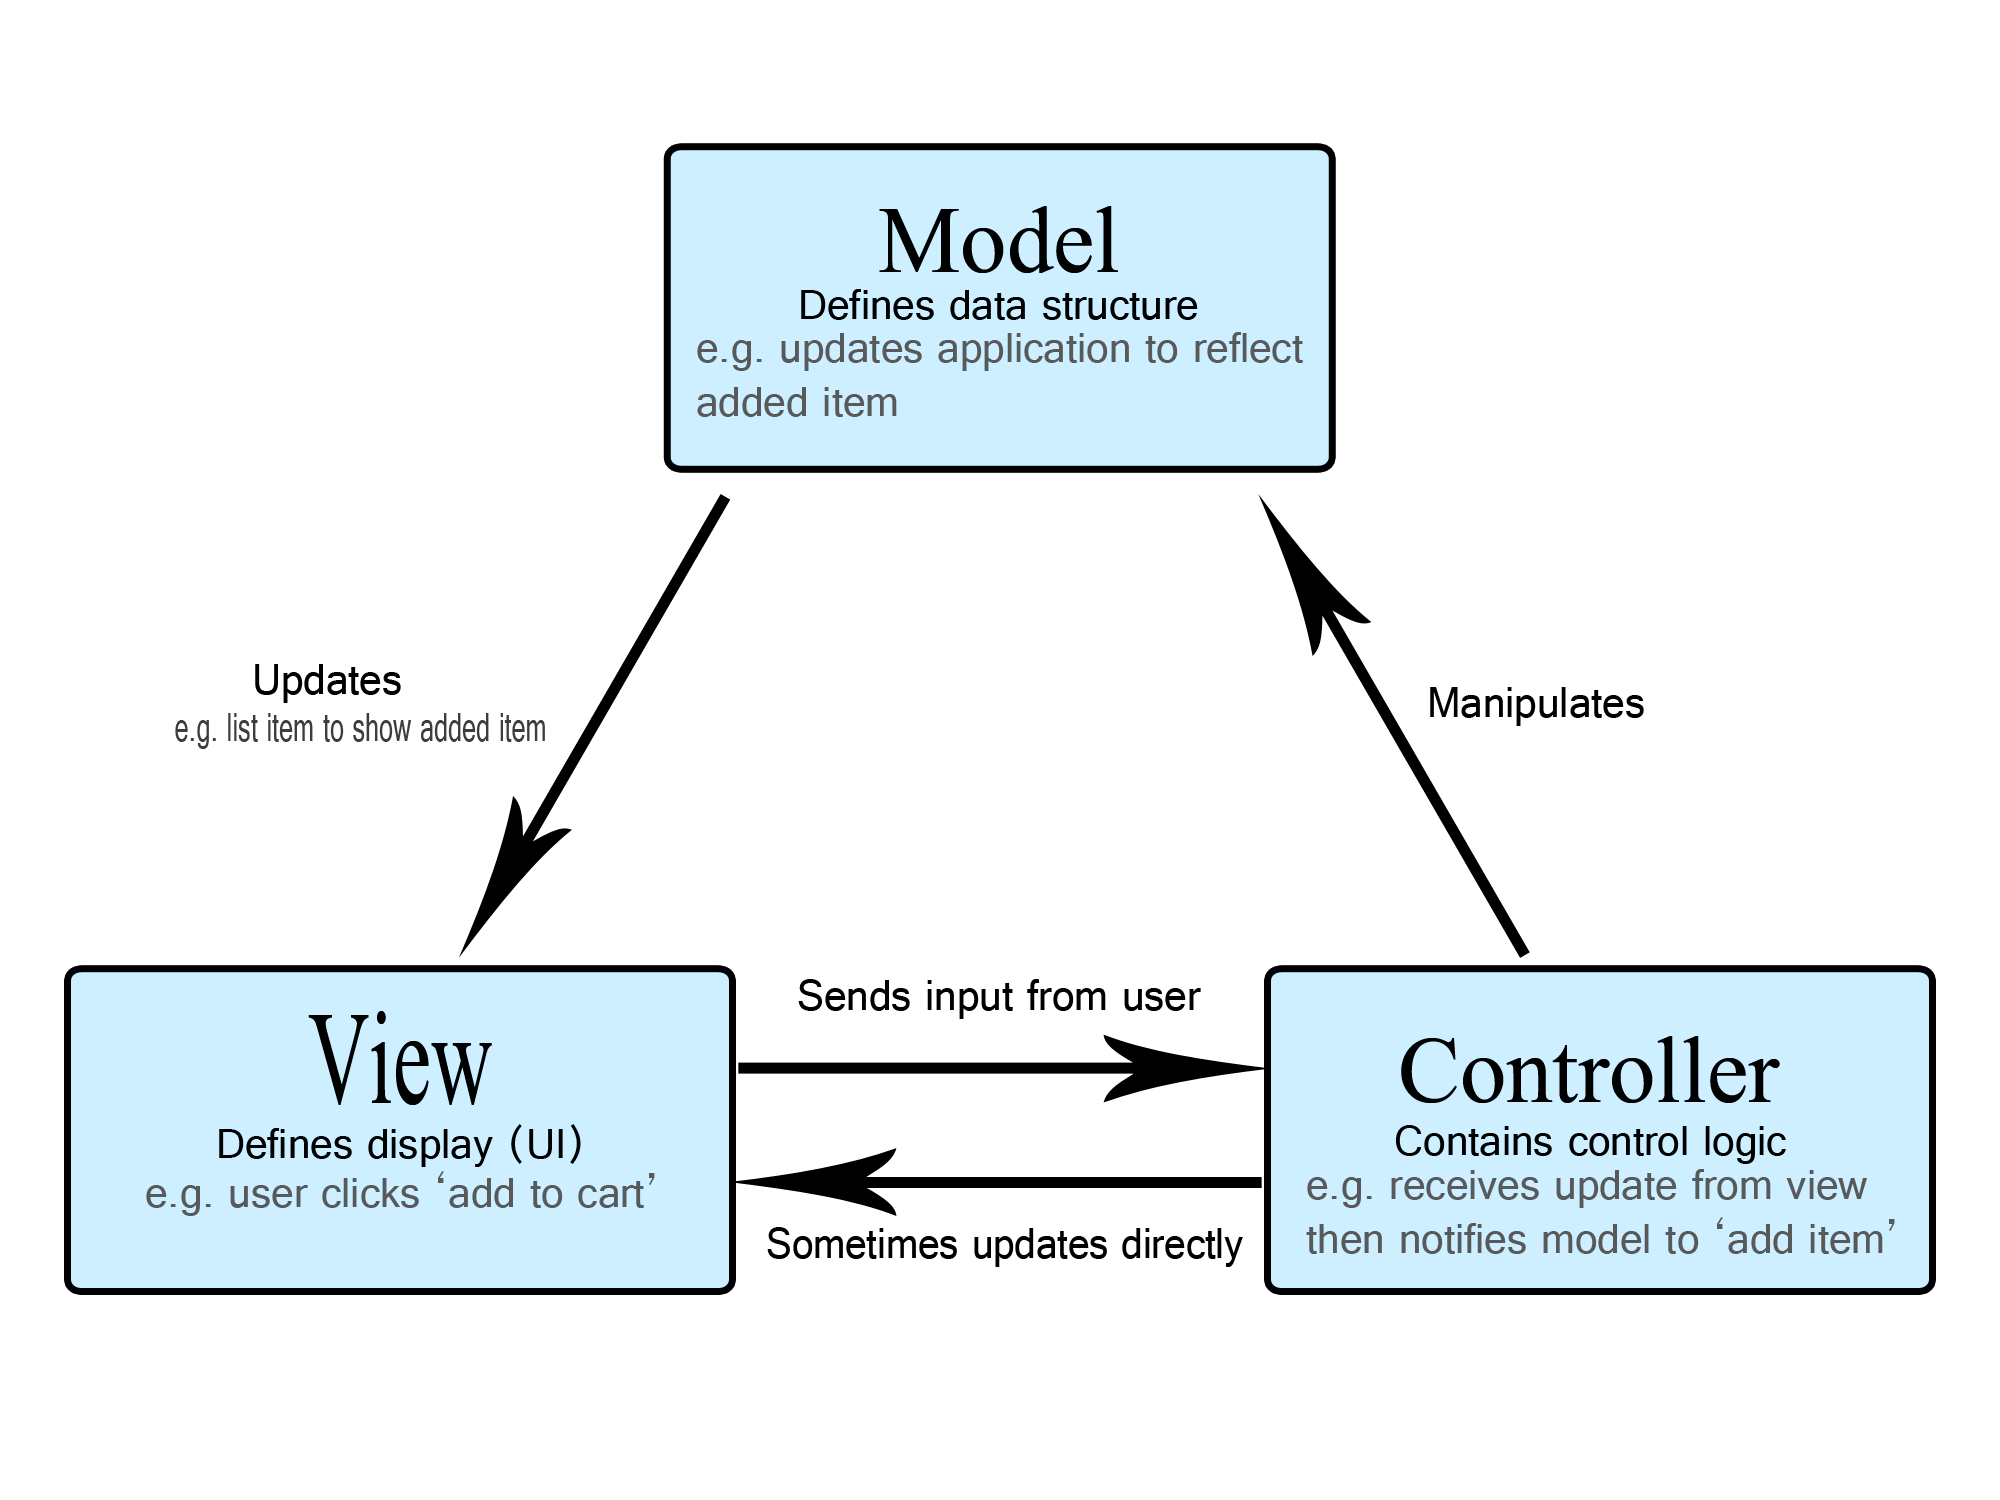
\includegraphics[scale=0.8]{graphics/model-view-controller-light-blue.png}
			\caption{MVC pattern design \cite{mvc}}
			\label{fig:MVC}
	\end{figure}
    
    
    When it comes to designing the application, as a backend developer, I focus on 5 main components below:

    \begin{enumerate}
        \item \textbf{Modular Organization:} Flask blueprints allow the application to be divided into modular components, each representing a distinct feature or functionality. I designed Blueprints to facilitate organized code by grouping related routes, templates, and static files. They are essential for large applications, promoting code reuse and separation of concerns.

        \item \textbf{URL Mapping:} Routes define the URL patterns that the application responds to and associate them with specific controller functions. Flask uses the \textbf{@app.route} decorator together with the corresponding Blueprint to map URLs to view functions. I defined all routes (corresponding to specific endpoints) of the web application, they process requests and generate appropriate responses (Rest API).

        \item \textbf{Logic Implementation:} Controllers contain the core logic for handling requests, interacting with models, and preparing data for views. They validate input, execute business logic, and orchestrate the data flow between models and views. By centralizing the application's logic, controllers ensure a clear separation of concerns.

        \item \textbf{Data Representation:} Models represent 

        \item \textbf{Reusable Components:} Common shared functions include utility functions, helper methods, and services that are used across multiple parts of the application (file utilities, database utilities, etc.). These functions promote code reuse and reduce redundancy. I organized common shared functions into separate packages named \textbf{common/}, which can be imported wherever needed. 
    \end{enumerate}

   My tasks included implementing the API endpoints, encompassing routes, controllers, and models, which provided the necessary data for the frontend. These APIs featured several critical functionalities essential for the web application. Firstly, they facilitated the upload and import of Excel billing files, ensuring seamless data integration. Secondly, the APIs enabled the visualization of billing information, presenting data in an accessible and user-friendly manner. Additionally, they provided robust filtering options to allow users to efficiently search and sort billing information. Another key feature was the generation of report charts, offering graphical representations of billing data for better insights. Lastly, the APIs supported exporting reports, allowing users to download and utilize billing information in various formats for further analysis and record-keeping.

    \subsubsection{Challenges}
    Throughout the web application development, I encountered various challenges that necessitated significant time investment in resolving them, thereby enhancing my technical proficiency.

    \begin{enumerate}
        \item \textbf{Requirement changes: } During the development phase, the requirements for the end-user interfaces and various features have changed. These changes in requirements significantly impacts the scope, timeline, and direction of the project. \\ 
        % Developers must be prepared to handle these changes efficiently and effectively.
        \textbf{\underline{Solution:}} Our team works with stakeholders to prioritize changes based on their impact and feasibility. This helps in focusing on high-value features and prevents the project from becoming overwhelming. Effective scope management ensures that critical requirements are addressed first, while less important changes can be scheduled for later.
        
        \item \textbf{Primary key constraints size limitation:} In the context of database development, the challenge arose from constraints on the size of primary keys imposed by the MySQL DBMS. \\ 
        \textbf{\underline{Solution:}} Consequently, a reassessment of the size allocation for each attribute across database entities became necessary.

        \item \textbf{Concurrency issues:} Another challenge involved concurrency issues arising from simultaneous attempts by users to upload billing excel files while other upload processes were ongoing. Resolving these issues necessitated establishing communication and coordination between these processes. \\ 
        \textbf{\underline{Solution:}} To address this, I implemented a solution using shared files. When an upload process initiates, it creates a file named \textbf{upload\_running}. Upon completion of the upload process, this file is subsequently removed. Therefore, subsequent upload processes are designed to first check for the existence of this file in the system, determining their execution based on its presence or absence.


        \item \textbf{Training for new members:} As a backend developer working on the web application project, introducing new features often necessitates bringing new team members on board to meet deadlines and ensure timely delivery. I had to ensure that new members quickly acquired the necessary knowledge about the project’s architecture, existing features, and coding standards. \\ 
        \textbf{\underline{Solution:}} Creating comprehensive and up-to-date documentation is crucial. This includes detailed architecture diagrams, API documentation, coding guidelines, and setup instructions. A well-maintained knowledge base allows new developers to self-study and reference materials as needed. Additionally, I assigned small and manageable tasks that created a supportive and efficient training environment for new members.
    \end{enumerate}


    \subsubsection{Delivery documentations}
    For the web application project, I have produced two essential documents. The first document details the API specifications using Swagger, ensuring clarity and accessibility in API implementation. The second document encompasses comprehensive guidelines for project requirements, setup procedures, and development practices. These documents aim to streamline communication, facilitate seamless integration of functionalities, and provide clear, structured guidance for efficient project development and deployment.

    

\subsection{Project output}

During my ongoing involvement in the project, I have continued to receive positive feedback from my manager regarding the code structures I have implemented and the maintenance of the project's current flow. \\

\noindent The consistency and usability of the APIs across different functionalities within the project have been notable. They have facilitated seamless integration and ease of use, contributing significantly to the overall project success. Furthermore, optimizations in database query performance have resulted in enhanced efficiency, thereby improving the user experience by ensuring quicker response times and smoother data retrieval processes. \\

\noindent The positive reception and feedback received from colleagues underscore the impact of these improvements on project outcomes. Their validation serves as a testament to the effectiveness of the technical solutions implemented. Successfully integrating and deploying backend server functionalities has further solidified my contribution to the project's objectives. This achievement reflects a combination of strategic planning, meticulous implementation, and effective collaboration with team members. \\

\noindent Looking ahead, I am committed to continuing to leverage and expand upon my skills and expertise. By staying attuned to emerging technologies and industry best practices, I aim to further enhance the project's capabilities and maintain its trajectory of success. My dedication to ongoing learning and proactive problem-solving will ensure that I continue to deliver meaningful contributions and drive continuous improvement in future endeavors.


%\section{Internship Result}

\subsection{Internship target and expectation}

During my internship at BGSW Vietnam, my primary target was to bridge the gap between theoretical knowledge and practical application in the realm of web application development. I aimed to gain hands-on experience with industry-standard tools and technologies, such as Python, Flask, SQLAlchemy, and front-end frameworks. My expectations included enhancing my programming skills, understanding the full software development lifecycle, and learning to collaborate effectively within a team environment. Additionally, I sought to develop strong problem-solving abilities by tackling real-world challenges and to understand the best practices for code quality, testing, and deployment. I also anticipated gaining insights into agile methodologies and improving my ability to manage tasks and timelines efficiently. Overall, my goal was to emerge from this internship with a solid foundation in web application development and a clear understanding of the dynamics of working in a professional software development setting.

\subsection{Internship output}

Upon completing my internship at BGSW Vietnam, I have successfully achieved and exceeded my initial targets and expectations. I played a crucial role in the development of a comprehensive web application project, contributing significantly to both backend and frontend development. I developed proficiency in utilizing the Flask framework to build robust APIs, and I enhanced my skills in database management with SQLAlchemy. I also gained experience with version control using Git, and I learned how to use Docker for containerization, ensuring that our development environment was consistent and scalable. My problem-solving skills were honed as I addressed various technical challenges, such as optimizing database queries and handling concurrency issues. The internship also provided me with valuable experience in writing documentation, including API documentation with Swagger and setup guides for deployment. The positive feedback from my mentors and peers, along with the successful completion of project milestones, indicates that I have made a substantial contribution to the team. This experience has significantly boosted my confidence in my technical and collaborative abilities.

\subsection{Future path}
My immediate goal is to secure a software developer position where I can continue to refine my skills and contribute to impactful projects. I am particularly interested in roles that involve web application development, cloud computing, and data management, as these areas align with the expertise I developed during my internship. In the long term, I aspire to become a full-stack developer, capable of designing and implementing complex applications from front-end to back-end. I plan to pursue continuous learning through professional development courses, certifications, and staying updated with emerging technologies and industry trends. Additionally, I am motivated to contribute to open-source projects and participate in tech communities to broaden my knowledge and network. Ultimately, I aim to leverage my skills to create innovative solutions that address real-world problems, drive business success, and enhance user experiences.





%\section{Conclusion}

This report presents the outcomes of the internship program undertaken at BGSW Vietnam, selected to fulfill the practical training requirements as an IT Developer. Throughout the internship duration, active involvement in technical skills training and engagement in the web application project constituted significant aspects of the experience. This comprehensive training encompassed various facets of software development, from backend and frontend programming to database design and system integration, providing a holistic view of the development lifecycle. \\

\noindent Engagement in the web application project was particularly enriching. It allowed for the application of theoretical knowledge to real-world scenarios, enhancing my problem-solving abilities and technical proficiency. Working on tasks such as designing database schemas, implementing API endpoints, and optimizing query performance offered practical insights into the complexities of software development. The collaborative environment at BGSW Vietnam further augmented my learning, as I received constructive feedback from mentors and collaborated with team members, fostering an atmosphere of continuous improvement. \\

\noindent The amalgamation of these factors facilitated a rich and rewarding experience within the scope of the internship program. The skills and knowledge acquired during this period have significantly bolstered my readiness to tackle professional challenges in the software development field. The internship at BGSW Vietnam has not only solidified my technical foundation but also instilled a sense of confidence and preparedness to contribute effectively to future projects. As I move forward, the experiences and lessons learned during this internship will undoubtedly serve as a cornerstone for my career development, guiding me in my journey as an aspiring software developer.
%\section{Appendix}

% % citation - references
\bibliographystyle{plainurl}
\bibliography{refs.bib}
\nocite{*}

% \include{chapters/2_introduction.tex}
% \include{chapters/3_language.tex}
% \include{chapters/4_integrationwolang.tex}
% \include{chapters/5_life.tex}
% \section{Conclusion and Future Work}


\subsection{Conclusion}

In conclusion, the Student Life Support Service web application represents a significant advancement in the way students can access and manage essential resources. By leveraging modern technologies such as ReactJS, Material UI, NodeJS, and PostgreSQL, the application provides a robust and responsive platform that meets the dynamic needs of its users. The use of ReactJS enables the creation of a seamless user interface, fostering an intuitive navigation experience. Material UI enhances this by offering a comprehensive set of pre-designed components that streamline the development process and maintain a consistent aesthetic across the application. \\ \\
The backend, built with NodeJS and ExpressJS, ensures efficient data handling and real-time interactions through the implementation of SocketIO. This combination allows for swift processing of requests and timely updates, critical for a platform designed to support communication among students and staff. PostgreSQL's strong ACID compliance guarantees the integrity and reliability of data, which is crucial for managing sensitive information such as user accounts and communication logs. \\ \\
Throughout the development process, extensive attention has been paid to user experience. The application is designed to be responsive, catering to various devices and screen sizes, which is essential in today’s mobile-first world. Furthermore, thorough testing and validation have been conducted to ensure the application functions smoothly, providing users with a dependable resource for support and information. \\ \\
Looking ahead, the project has laid a strong foundation for future enhancements. As the needs of students evolve and grow, so too must the capabilities of the application. By focusing on areas such as dynamic role management, scalability, and improved handling of concurrent user requests, the Student Life Support Service can adapt to changing user demands while ensuring high performance and security. \\ \\
In essence, the development of this web application is not merely an endpoint but the beginning of an ongoing journey. The commitment to continuous improvement will ensure that the platform remains relevant and valuable to students, supporting their academic and social endeavors in an increasingly digital world. With a clear vision for future enhancements and a solid technical foundation, the Student Life Support Service is poised to significantly impact student life on campus, promoting engagement and accessibility like never before.

\subsection{Future Work}
There are several key areas for improvement and expansion have been identified in the future:

	\begin{enumerate}
		\item \textbf{Dynamic Role Management:} Implementing a dynamic role management system will enhance the application’s flexibility. This feature will allow administrators to create and assign specific permissions to different user roles, tailoring access and functionality based on user needs. By enabling fine-grained control over resource access, the system can better accommodate various user requirements and enhance security.
		
		\item \textbf{Scalability:} To ensure the application can handle a growing number of users and increased data load, scalability must be a primary focus. This involves optimizing the architecture to support horizontal scaling, which can be achieved by implementing load balancers and distributing requests across multiple server instances. Additionally, strategies such as microservices architecture can be explored to further enhance scalability and maintainability.
		
%		\item \textbf{Handling High Concurrent User Requests:} Improving the application’s ability to handle high volumes of simultaneous user requests is crucial for maintaining performance and user satisfaction. Techniques such as caching strategies (using Redis or similar technologies) can significantly reduce database load and improve response times. Additionally, optimizing database queries and utilizing connection pooling can further enhance the system's efficiency under heavy load.
	\end{enumerate}
	
\noindent By addressing these future work areas, the Student Life Support Service web application can continue to evolve and better serve its users in reality, ensuring a reliable and efficient platform for student engagement and support.



% citation - references
% \printbibliography
\bibliographystyle{plainurl}
\bibliography{refs.bib}
\nocite{*}


\end{document}